
%%%%%%%%%%%%%%
%% Run LaTeX on this file several times to get Table of Contents,
%% cross-references, and citations.

%% If you have font problems, you may edit the w-bookps.sty file
%% to customize the font names to match those on your system.

%% w-bksamp.tex. Current Version: Feb 16, 2012
%%%%%%%%%%%%%%%%%%%%%%%%%%%%%%%%%%%%%%%%%%%%%%%%%%%%%%%%%%%%%%%%
%
%  Sample file for
%  Wiley Book Style, Design No.: SD 001B, 7x10
%  Wiley Book Style, Design No.: SD 004B, 6x9
%
%
%  Prepared by Amy Hendrickson, TeXnology Inc.
%  http://www.texnology.com
%%%%%%%%%%%%%%%%%%%%%%%%%%%%%%%%%%%%%%%%%%%%%%%%%%%%%%%%%%%%%%%%

%%%%%%%%%%%%%
% 7x10
%\documentclass{wileySev}

% 6x9
\documentclass{wileySix}

\usepackage{graphicx}
\usepackage{listings}

\usepackage{color}
 
\definecolor{codegreen}{rgb}{0,0.6,0}
\definecolor{codegray}{rgb}{0.5,0.5,0.5}
\definecolor{codepurple}{rgb}{0.58,0,0.82}
\definecolor{backcolour}{rgb}{0.95,0.95,0.92}
 
\lstdefinestyle{mystyle}{
    backgroundcolor=\color{backcolour},   
    commentstyle=\color{codegreen},
    keywordstyle=\color{magenta},
    numberstyle=\tiny\color{codegray},
    stringstyle=\color{codepurple},
    basicstyle=\footnotesize,
    breakatwhitespace=false,         
    breaklines=true,                 
    captionpos=b,                    
    keepspaces=true,                 
    numbers=left,                    
    numbersep=5pt,                  
    showspaces=false,                
    showstringspaces=false,
    showtabs=false,                  
    tabsize=2,
    language=sh
}
 
\lstset{style=mystyle}

%%%%%%%
%% for times math: However, this package disables bold math (!)
%% \mathbf{x} will still work, but you will not have bold math
%% in section heads or chapter titles. If you don't use math
%% in those environments, mathptmx might be a good choice.

% \usepackage{mathptmx}

% For PostScript text
\usepackage{w-bookps}

%%%%%%%%%%%%%%%%%%%%%%%%%%%%%%%%%%%%%%%%%%%%%%%%%%%%%%%%%%%%%%%%
%% Other packages you might want to use:

% for chapter bibliography made with BibTeX
% \usepackage{chapterbib}

% for multiple indices
% \usepackage{multind}

% for answers to problems
% \usepackage{answers}

%%%%%%%%%%%%%%%%%%%%%%%%%%%%%%
%% Change options here if you want:
%%
%% How many levels of section head would you like numbered?
%% 0= no section numbers, 1= section, 2= subsection, 3= subsubsection
%%==>>
\setcounter{secnumdepth}{3}

%% How many levels of section head would you like to appear in the
%% Table of Contents?
%% 0= chapter titles, 1= section titles, 2= subsection titles, 
%% 3= subsubsection titles.
%%==>>
\setcounter{tocdepth}{2}

%% Cropmarks? good for final page makeup
%% \docropmarks

%%%%%%%%%%%%%%%%%%%%%%%%%%%%%%
%
% DRAFT
%
% Uncomment to get double spacing between lines, current date and time
% printed at bottom of page.
% \draft
% (If you want to keep tables from becoming double spaced also uncomment
% this):
% \renewcommand{\arraystretch}{0.6}
%%%%%%%%%%%%%%%%%%%%%%%%%%%%%%

%%%%%%% Demo of section head containing sample macro:
%% To get a macro to expand correctly in a section head, with upper and
%% lower case math, put the definition and set the box 
%% before \begin{document}, so that when it appears in the 
%% table of contents it will also work:

\newcommand{\VT}[1]{\ensuremath{{V_{T#1}}}}

%% use a box to expand the macro before we put it into the section head:

\newbox\sectsavebox
\setbox\sectsavebox=\hbox{\boldmath\VT{xyz}}

%%%%%%%%%%%%%%%%% End Demo


\begin{document}


\booktitle{Dasar Dasar OpenCV}
\subtitle{Cerdas Mengoprasikan Gambar}

\authors{Faisal Najib Abdullah\\
\affil{Informatics Research Center}
%Floyd J. Fowler, Jr.\\
%\affil{University of New Mexico}
}

\offprintinfo{Dasar Dasar OpenCV, First Edition}{Faisal Najib Abdullah}

%% Can use \\ if title, and edition are too wide, ie,
%% \offprintinfo{Survey Methodology,\\ Second Edition}{Robert M. Groves}

%%%%%%%%%%%%%%%%%%%%%%%%%%%%%%
%% 
\halftitlepage

\titlepage


%\begin{copyrightpage}{2019}
\i%nput{info/copyrightpage}
%\end{copyrightpage}

\dedication{`Jika Kamu tidak dapat menahan lelahnya belajar, 
Maka kamu harus sanggup menahan perihnya Kebodohan.'
~Imam Syafi'i~}

\begin{contributors}
\name{Faisal Najib Abdullah,} Informatics Research Center., Politeknik Pos Indonesia, Bandung,
Indonesia



\end{contributors}

\contentsinbrief
\tableofcontents
\listoffigures
\listoftables
\lstlistoflistings


\begin{foreword}
Sepatah kata dari Kaprodi, Kabag Kemahasiswaan dan Mahasiswa
\end{foreword}

\begin{preface}
Buku ini diciptakan bagi pengembang yang ingin mengembangkan kemampuan memprogram di bahasa python menggunakan library opencv.

\prefaceauthor{Faisal Najib Abdullah}
\where{Bandung, Jawa Barat\\
Januari, 2020}
\end{preface}


\begin{acknowledgments}
Terima kasih atas masukan dari pembimbing agar bisa membuat buku ini 
lebih baik dan lebih mudah dimengerti.

Terima kasih ini juga ditujukan khusus untuk team IRC yang 
telah fokus untuk belajar dan memahami bagaimana buku ini mendampingi proses 
Belajar.
\authorinitials{R. M. A.}
\end{acknowledgments}

\begin{acronyms}
\acro{AI}{Artificial Intelligence}
\acro{ETL}{Extract Transform Load}
\acro{NLP}{Natural Language Processing}

\end{acronyms}

%\begin{glossary}
%\term{cybernetics}Adalah sistem yang berinteraksi langsung dengan diri sendiri yang memahami dan menentukan proses tujuan.

\term{Heuristik}Adalah sebuah metode yang mengembangkan efisiensi dalam proses pencarian.

\term{Supervised}Adalah sebuah tugas pengumpulan data untuk menyimpulkan fungsi dari data pelatihan berlabel.

\term{Unsupervised}Adalah Tidak adanya memiliki data latih, sehingga dari data yang ada kita mengelompokan data tersebut menjadi 2 ataupun 3 bagian.

%\end{glossary}

\begin{symbols}
\term{A}Amplitude

\term{\hbox{\&}}Propositional logic symbol 

\term{a}Filter Coefficient

\bigskip

\term{\mathcal{B}}Number of Beats
\end{symbols}

\begin{introduction}

%% optional, but if you want to list author:

\introauthor{Faisal Najib Abdullah}
{Informatics Research Center\\
Bandung, Jawa Barat, Indonesia}

Pada era disruptif  \index{disruptif}\index{disruptif!modern} 
saat ini. Pemrograman merupakan sebuah kebutuhan dalam sebuah organisasi pengembangan perangkat lunak.
Buku ini diharapkan bisa menjadi penghantar para programmer, analis, IT Operation dan Project Manajer.
Dalam melakukan implementasi program pada diri dan organisasinya.

Rumusnya cuman sebagai contoh aja biar keren.

\begin{equation}
ABC {\cal DEF} \alpha\beta\Gamma\Delta\sum^{abc}_{def}
\end{equation}

\end{introduction}

%%%%%%%%%%%%%%%%%%Isi Buku_

\chapter{Pengenalan OpenCV}
\section{OpenCV}
\subsection{Definisi OpenCV}
	
	Computer Vision adalah ilmu pemrograman komputer untuk memproses dan pada akhirnya memahami gambar dan video, atau hanya mengatakan membuat komputer melihatnya. Memecahkan sebagian kecil dari tantangan Visi Komputer tertentu, menciptakan kemungkinan baru yang menarik dalam teknologi, teknik, dan bahkan hiburan. Untuk memajukan penelitian visi dan menyebarkan pengetahuan visi, sangat penting untuk memiliki perpustakaan fungsi pemrograman dengan kode yang dioptimalkan dan portabel, dan mudah-mudahan tersedia secara gratis. Ini adalah tujuan asli tim Intel pada tahun 1999 ketika OpenCV (Open Source Computer Vision Library) secara resmi diluncurkan. Sejak itu, sejumlah programmer telah berkontribusi pada perkembangan perpustakaan terbaru. Perubahan besar terbaru terjadi pada tahun 2009 (OpenCV 2) yang mencakup perubahan utama pada antarmuka C ++. Rilis perpustakaan terbaru dapat ditemukan di situs web resmi OpenCV. Saat ini perpustakaan memiliki> 2500 algoritma yang dioptimalkan. Ini digunakan secara luas di seluruh dunia, memiliki> 2,5 juta unduhan dan> 40 ribu orang di grup pengguna. OpenCV dapat digunakan dalam aplikasi akademik dan komersial juga, di bawah lisensi BSD. Untuk menguasai setiap elemen pustaka OpenCV perlu berkonsultasi dengan banyak buku yang tersedia tentang topik OpenCV. Namun demikian, membaca materi yang lebih komprehensif seperti itu harus lebih mudah setelah memahami ide dasar tentang OpenCV dari makalah ini. Bahkan untuk membuatnya lebih nyaman, teks yang disajikan di sini dengan cermat mengikuti salah satu sumber OpenCV terbaru.

	OpenCV adalah pustaka Pengolah Gambar yang dibuat oleh Intel, dapat diunduh secara bebas dan tersedia untuk C, C ++, Java dan Python, Windows, Linux, Mac OS, iOS dan Android Terbaru Versi-versinya adalah opencv2.4.13 dan opencv-3.1. Ini adalah Sumber terbuka dan juga Mudah digunakan dan diinstal. Ini dirancang untuk efisiensi komputasi fokus yang kuat pada aplikasi waktu nyata Implementasi pertama adalah dalam bahasa pemrograman C; Namun, popularitasnya tumbuh dengan implementasi C ++ pada Versi 2.0. Fungsi baru diprogram dengan C ++. Namun, saat ini, perpustakaan memiliki antarmuka penuh untuk bahasa pemrograman lain, seperti Java, Python, dan MATLAB / Octave. OpenCV tersedia secara bebas untuk diunduh di http://opencv.org. Situs ini menyediakan versi terakhir untuk distribusi (saat ini, 3.0 beta) dan versi yang lebih lama. OpenCV mengharuskan gambar dalam BGR atau Grayscale untuk ditampilkan atau disimpan. Kalau tidak, efek yang tidak diinginkan dapat terjadi.

	Pustaka OpenCV (sejak versi 2.2) dibagi menjadi beberapa modul, di mana setiap modul dapat dipahami, secara umum, sebagai didedikasikan untuk satu kelompok masalah penglihatan komputer. Semua kelas dan fungsi didefinisikan dalam ruang nama cv. Oleh karena itu untuk mengaksesnya kita dapat mendahului definisi fungsi utama dengan deklarasi menggunakan namespace cv; atau awali nama kelas dan fungsi OpenCV berdasarkan spesifikasi namespace cv. Objek utama adalah Mat kelas. Seperti dilibatkan oleh nama kelas itu pada dasarnya adalah sebuah matriks yang memegang nilai-nilai piksel dari beberapa gambar dan, di samping itu, sejumlah atribut tentang suatu gambar. Dalam kasus yang paling sederhana, sebuah gambar dapat dibuat sebagai cv :: Mat image ;, membuat gambar dengan ukuran 0 x 0. Mungkin variabel anggota yang paling penting dari objek gambar adalah data di mana anggota image.data sebenarnya adalah penunjuk ke memori yang dialokasikan blok yang berisi data gambar (dalam kasus sepele ini adalah image.data = 0). Atau selama pembuatan objek Mat kita bisa secara eksplisit menentukan ukuran awal dan jenis setiap elemen matriks. Jenis ini menentukan, misalnya, menandatangani nilai gambar piksel 1-byte, atau tiga saluran untuk gambar berwarna , atau bahkan angka titik apung 32-bit atau 64bit.

	Setelah objek matematika kelas didefinisikan, fitur yang bagus tentangnya (tidak ada dalam versi awal OpenCV) adalah bahwa alokasi / deallokasi memori dilakukan secara otomatis. Misalnya, memori yang secara otomatis dialokasikan selama gambar dibacakan ke beberapa objek, juga akan secara otomatis dirilis setelah objek yang sesuai keluar dari ruang lingkup. Hal penting lainnya adalah bahwa kelas Mat mengimplementasikan penghitungan referensi dan salinan dangkal. Oleh karena itu, ketika gambar ditugaskan ke yang lain, data gambar itu sendiri tidak disalin dan kedua gambar menunjuk ke blok memori yang sama (ini juga berlaku untuk gambar yang dilewati / dikembalikan oleh nilai). Namun, karena jumlah referensi didukung, memori yang dialokasikan untuk data gambar (piksel) itu sendiri akan dirilis hanya ketika semua referensi ke gambar dihancurkan.

	Dalam versi sebelum OpenCV 2, fungsi dan struktur seperti C digunakan (masih bisa jadi) dan struktur utama adalah IplImage. Meskipun ada cara mudah untuk mengubah struktur IplImage menjadi objek cv :: Mat, sangat disarankan untuk menghindari struktur data yang sudah usang ini.

\newpage
\subsection{Sejarah Kecerdasan Opencv}
    Resmi diluncurkan pada tahun 1999, proyek OpenCV pada awalnya merupakan inisiatif Intel Research untuk memajukan aplikasi intensif CPU, bagian dari serangkaian proyek termasuk penelusuran sinar waktu nyata dan dinding layar 3D. Kontributor utama untuk proyek ini termasuk sejumlah pakar optimisasi di Intel Rusia, serta Tim Perpustakaan Kinerja Intel. Pada hari-hari awal OpenCV, tujuan proyek digambarkan sebagai:

    \begin{enumerate}
	\item Memajukan penelitian visi dengan menyediakan tidak hanya kode terbuka tetapi juga dioptimalkan untuk infrastruktur visi dasar. Tidak ada lagi menciptakan kembali roda.
	\item Menyebarkan pengetahuan visi dengan menyediakan infrastruktur umum yang dapat dibangun oleh pengembang, sehingga kode akan lebih mudah dibaca dan dapat ditransfer.
	\item Aplikasi komersial berbasis visi mutakhir dengan membuat kode portabel yang dioptimalkan kinerja tersedia secara gratis - dengan lisensi yang tidak memerlukan kode untuk terbuka atau bebas sendiri.
	\end{enumerate} 

	Versi alpha pertama dari OpenCV dirilis ke publik di Konferensi IEEE pada Computer Vision dan Pattern Recognition pada tahun 2000, dan lima beta dirilis antara tahun 2001 dan 2005. Versi 1.0 pertama dirilis pada tahun 2006. Versi 1.1 "pra-rilis "dirilis pada Oktober 2008.

	Rilis utama kedua dari OpenCV adalah pada Oktober 2009. OpenCV 2 mencakup perubahan besar pada antarmuka C ++, yang bertujuan untuk lebih mudah, pola yang lebih aman, fungsi baru, dan implementasi yang lebih baik untuk yang sudah ada dalam hal kinerja (terutama pada multi- sistem inti). Rilis resmi sekarang terjadi setiap enam bulan dan pengembangan sekarang dilakukan oleh tim Rusia independen yang didukung oleh perusahaan komersial.

	Pada Agustus 2012, dukungan untuk OpenCV diambil alih oleh yayasan nirlaba OpenCV.org, yang mengelola pengembang dan situs pengguna.

	Pada Mei 2016, Intel menandatangani perjanjian untuk mengakuisisi Itseez, pengembang OpenCV terkemuka.

\newpage
\section{NumPy}
\subsection{Definisi NumPy}
NumPy adalah perpustakaan untuk bahasa pemrograman Python, menambahkan dukungan untuk array dan matriks multi-dimensi yang besar, bersama dengan koleksi besar fungsi matematika tingkat tinggi untuk beroperasi pada array ini. Nenek moyang NumPy, Numeric, pada awalnya diciptakan oleh Jim Hugunin dengan kontribusi dari beberapa pengembang lainnya. Pada 2005, Travis Oliphant menciptakan NumPy dengan memasukkan fitur-fitur Numarray yang bersaing ke Numeric, dengan modifikasi ekstensif. NumPy adalah perangkat lunak sumber terbuka dan memiliki banyak kontributor.

\subsection{Sejarah NumPy}
Bahasa pemrograman Python pada awalnya tidak dirancang untuk komputasi numerik, tetapi menarik perhatian komunitas ilmiah dan teknik sejak awal, sehingga kelompok minat khusus yang disebut matrix-sig didirikan pada tahun 1995 dengan tujuan mendefinisikan paket komputasi array. Di antara anggotanya adalah desainer dan pengelola Python, Guido van Rossum, yang menerapkan ekstensi ke sintaksis Python (khususnya sintaks pengindeksan) untuk membuat komputasi array lebih mudah.

Implementasi dari paket matriks diselesaikan oleh Jim Fulton, kemudian digeneralisasi oleh Jim Hugunin menjadi Numeric, juga beragam disebut ekstensi Numerical Python atau NumPy. Hugunin, seorang mahasiswa pascasarjana di Massachusetts Institute of Technology (MIT), bergabung dengan Corporation for National Research Initiatives (CNRI) untuk bekerja pada JPython pada tahun 1997 meninggalkan Paul Dubois dari Lawrence Livermore National Laboratory (LLNL) ke ambil alih sebagai pengelola. Kontributor awal lainnya termasuk David Ascher, Konrad Hinsen dan Travis Oliphant.

Paket baru bernama Numarray ditulis sebagai pengganti Numeric yang lebih fleksibel. Seperti Numeric, sekarang sudah usang. Numarray memiliki operasi lebih cepat untuk array besar, tetapi lebih lambat daripada Numeric pada array kecil, jadi untuk sementara waktu kedua paket digunakan untuk kasus penggunaan yang berbeda. Versi terakhir Numeric v24.2 dirilis pada 11 November 2005 dan numarray v1.5.2 dirilis pada 24 Agustus 2006.

Ada keinginan untuk memasukkan Numeric ke dalam pustaka standar Python, tetapi Guido van Rossum memutuskan bahwa kodenya tidak dapat dipertahankan dalam keadaannya saat itu.

Pada awal 2005, pengembang NumPy Travis Oliphant ingin menyatukan komunitas sekitar satu paket array dan mem-porting fitur Numarray ke Numeric, merilis hasilnya sebagai NumPy 1.0 pada 2006. Proyek baru ini adalah bagian dari SciPy. Untuk menghindari menginstal paket SciPy besar hanya untuk mendapatkan objek array, paket baru ini dipisahkan dan disebut NumPy. Dukungan untuk Python 3 ditambahkan pada 2011 dengan NumPy versi 1.5.0.

Pada tahun 2011, PyPy memulai pengembangan penerapan API NumPy untuk PyPy. Ini belum sepenuhnya kompatibel dengan NumPy.

\subsection{Perkembangan NumPy}
NumPy menargetkan implementasi referensi CPython dari Python, yang merupakan penerjemah bytecode yang tidak mengoptimalkan. Algoritma matematika yang ditulis untuk versi Python ini sering berjalan jauh lebih lambat daripada yang dikompilasi setara. NumPy mengatasi masalah kelambatan sebagian dengan menyediakan array multidimensi dan fungsi dan operator yang beroperasi secara efisien pada array, membutuhkan penulisan ulang beberapa kode, sebagian besar loop internal menggunakan NumPy.

Menggunakan NumPy dalam Python memberikan fungsionalitas yang sebanding dengan MATLAB karena keduanya diinterpretasikan, dan keduanya memungkinkan pengguna untuk menulis program cepat selama sebagian besar operasi bekerja pada array atau matriks, bukan skalar. Sebagai perbandingan, MATLAB menawarkan sejumlah besar kotak alat tambahan, terutama Simulink, sedangkan NumPy secara intrinsik terintegrasi dengan Python, bahasa pemrograman yang lebih modern dan lengkap. Selain itu, paket Python komplementer tersedia; SciPy adalah pustaka yang menambahkan lebih banyak fungsi seperti MATLAB dan Matplotlib adalah paket merencanakan yang menyediakan fungsi merencanakan seperti MATLAB. Secara internal, baik MATLAB dan NumPy mengandalkan BLAS dan LAPACK untuk perhitungan aljabar linier yang efisien.

Binding Python dari perpustakaan visi komputer yang banyak digunakan OpenCV memanfaatkan array NumPy untuk menyimpan dan beroperasi pada data. Karena gambar dengan banyak saluran hanya direpresentasikan sebagai array tiga dimensi, pengindeksan, pemotongan atau penutupan dengan array lainnya adalah cara yang sangat efisien untuk mengakses piksel tertentu dari suatu gambar. Array NumPy sebagai struktur data universal dalam OpenCV untuk gambar, poin fitur yang diekstraksi, filter kernel dan banyak lagi yang sangat menyederhanakan alur kerja pemrograman dan debugging.

\textbf{Struktur data ndarray}
\newline
Fungsionalitas inti dari NumPy adalah ndarray, untuk susunan n-dimensional, struktur data. Array-array ini adalah pandangan yang melintas pada memori. Berbeda dengan struktur data daftar built-in Python (yang, meskipun namanya, adalah array dinamis), array ini diketik secara homogen: semua elemen dari array tunggal harus dari tipe yang sama.

Array tersebut juga dapat dilihat ke buffer memori yang dialokasikan oleh ekstensi C atau C plus plus, Cython, dan Fortran ke juru bahasa CPython tanpa perlu menyalin data, memberikan tingkat kompatibilitas dengan perpustakaan numerik yang ada. Fungsi ini dieksploitasi oleh paket SciPy, yang membungkus sejumlah perpustakaan seperti itu (terutama BLAS dan LAPACK). NumPy memiliki dukungan bawaan untuk ndarrays yang dipetakan di memori.

\textbf{Keterbatasan}
\newline
Memasukkan atau menambahkan entri ke sebuah array tidak sepele mungkin dengan daftar Python. Rutin np.pad untuk memperluas array sebenarnya membuat array baru dengan nilai bentuk dan padding yang diinginkan, menyalin array yang diberikan ke yang baru dan mengembalikannya. Operasi NumPy np.concatenate tidak benar-benar menghubungkan dua array tetapi mengembalikan yang baru, diisi dengan entri dari kedua array yang diberikan secara berurutan. Membentuk kembali dimensi array dengan np.reshape hanya mungkin selama jumlah elemen dalam array tidak berubah. Keadaan ini berasal dari fakta bahwa array NumPy harus dilihat pada buffer memori yang berdekatan. Paket pengganti yang disebut Blaze berupaya mengatasi batasan ini. 

Algoritma yang tidak dapat diekspresikan sebagai operasi vektor biasanya akan berjalan lambat karena mereka harus diimplementasikan dalam Python murni, sedangkan vektorisasi dapat meningkatkan kompleksitas memori dari beberapa operasi dari konstan ke linier, karena array sementara harus dibuat yang sama besarnya dengan input. Kompilasi kode numerik Runtime telah diterapkan oleh beberapa kelompok untuk menghindari masalah ini; solusi open source yang beroperasi dengan NumPy termasuk scipy.weave, numexpr dan Numba. Cython dan Pythran adalah alternatif kompilasi statis untuk ini.

\newpage
\subsection{Contoh Code Numpy}
Membuat Array menggunakan Numpy Python
\lstinputlisting{src/MembuatArray.py}

Operasi Sederhana Numpay
\lstinputlisting{src/OperasiSederhana.py}

Fungsi Universal Numpay
\lstinputlisting{src/UniversalFunction.py}

Aljabar Linear bagaimana memuat matriks menggunakan code numpay dengan mudah.
\lstinputlisting{src/LinearAlgebra.py}

Contoh penggabungan Numpay dengan Opencv.
\lstinputlisting{src/Penggabungan.py}	

\newpage
\section{Instalasi OpenCV}
\subsection{Instalasi pada Windows}

Windows tidak datang dengan Python yang sudah diinstal. Namun, wizard instalasi tersedia untuk Python, NumPy, SciPy, dan OpenCV yang telah dikompilasi. Atau, kita dapat membangun dari sumber. Sistem build OpenCV menggunakan CMake untuk konfigurasi dan Visual Studio atau MinGW untuk kompilasi.

Jika kami ingin dukungan untuk kamera kedalaman, termasuk Kinect, pertama-tama kita harus menginstal OpenNI dan SensorKinect, yang tersedia sebagai binari yang dikompilasi dengan wizard penginstalan. Kemudian, kita harus membangun OpenCV dari sumber.

\textbf{Catatan}

Versi OpenCV yang dikompilasi sebelumnya tidak menawarkan dukungan untuk kamera yang dalam. Pada Windows, OpenCV 2 menawarkan dukungan yang lebih baik untuk Python 32-bit daripada Python 64-bit. namun, dengan mayoritas komputer yang dijual hari ini menggunakan sistem 64-bit, instruksi kami akan merujuk pada 64-bit. Semua installer memiliki versi 32-bit yang tersedia dari situs yang sama dengan 64-bit.

\begin{enumerate}
	\item Beberapa langkah berikut merujuk pada pengeditan variabel PATH sistem. Tugas ini dapat dilakukan di jendela Variabel Lingkungan di Panel Kontrol.
	\item Pada Windows Vista / Windows 7 / Windows 8, klik menu Start dan luncurkan Panel Kontrol. Sekarang, navigasikan ke System and Security, Sistem, Pengaturan sistem lanjutan. Klik pada tombol Variabel Lingkungan….
	\item Pada Windows XP, klik pada menu Mulai dan navigasikan ke Control Panel | Sistem. Pilih tab Advanced. Klik pada tombol Variabel Lingkungan….
	\item Sekarang, di bawah System variable, pilih Path dan klik tombol Edit….
	\item Buat perubahan sesuai petunjuk.
	\item Untuk menerapkan perubahan, klik pada semua tombol OK (sampai kita kembali ke jendela utama Control Panel).
	\item Kemudian, keluar dan masuk kembali (atau reboot).
\end{enumerate}

\newpage
\textbf{Menggunakan penginstal biner (tidak ada dukungan untuk kamera kedalaman)}

Anda dapat memilih untuk menginstal Python dan pustaka terkait secara terpisah jika Anda mau; Namun, ada distribusi Python yang datang dengan installer yang akan mengatur seluruh tumpukan SciPy (yang mencakup Python dan NumPy), yang membuatnya sangat sepele untuk mengatur lingkungan pengembangan.
	
Salah satu distribusi tersebut adalah Anaconda Python (dapat diunduh di ). Setelah installer diunduh, jalankan dan ingat untuk menambahkan path ke instalasi Anaconda ke variabel PATH Anda mengikuti prosedur sebelumnya.

Berikut adalah langkah-langkah untuk mengatur Python7, NumPy, SciPy, dan OpenCV:
\begin{enumerate}
	\item Unduh dan instal 64 bit Python 3.7.1 dari \begin{verbatim} https://www.python.org/ftp/python/3.7.1/python-3.7.1-amd64.exe \end{verbatim}
		\begin{figure}[ht]
		\centering
		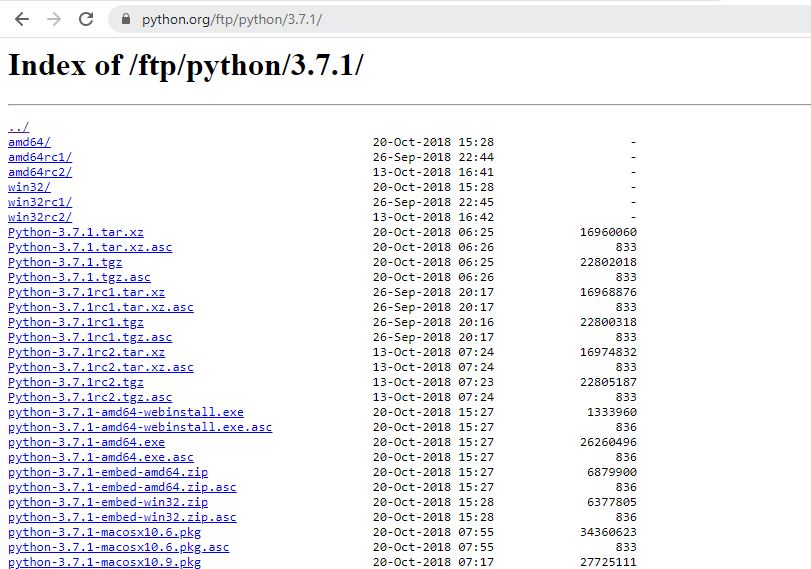
\includegraphics[scale=0.5]{figures/1,1.jpg}
		\caption{Download Python}
		\label{contoh}
		\end{figure}
\newpage
	\item Unduh dan instal NumPy 1.6.2.
		\begin{figure}[ht]
		\centering
		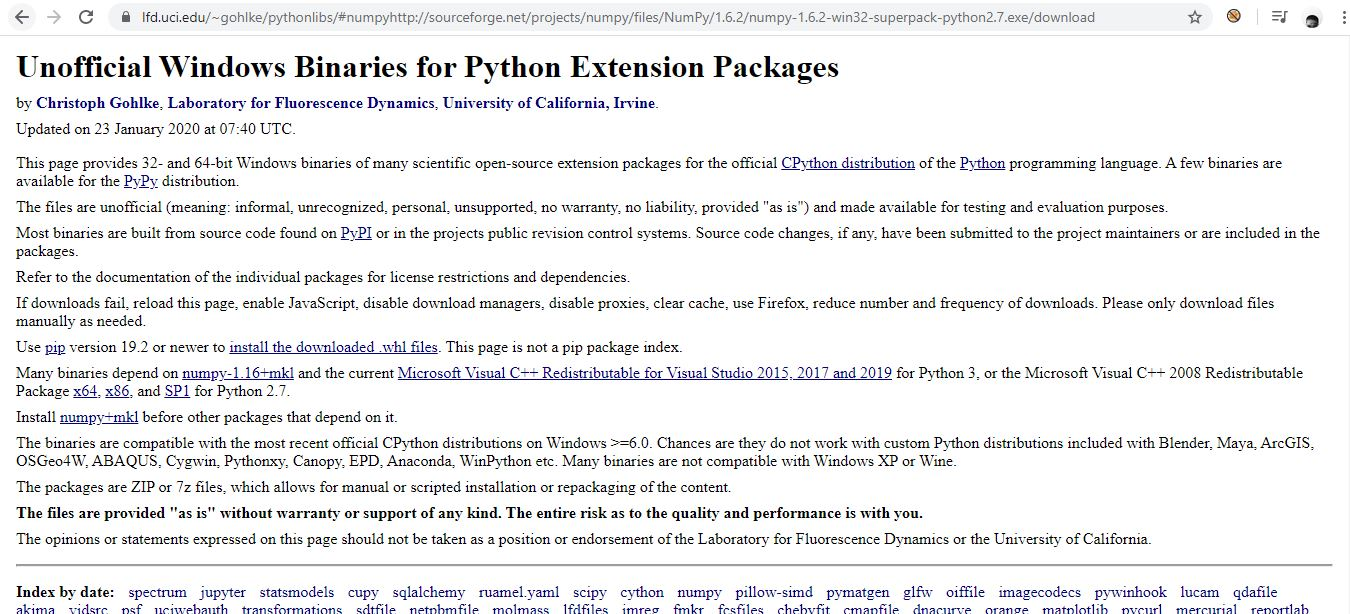
\includegraphics[scale=0.5]{figures/1,2.jpg}
		\caption{Cari Numpy terbaru pada wibsite ini}
		\label{contoh}
		\end{figure}
\newpage
	\item Unduh dan pasang SciPy 11.0 dari \begin{verbatim} http://www.lfd.uci.edu/~gohlke/pythonlibs/#scipyhttp://sourceforge.net/projects/scipy/files/scipy/0.11.0/scipy0.11.0win32-superpack-python2.7.exe/download \end{verbatim} (ini sama dengan NumPy dan ini adalah pemasang komunitas).
		\begin{figure}[ht]
		\centering
		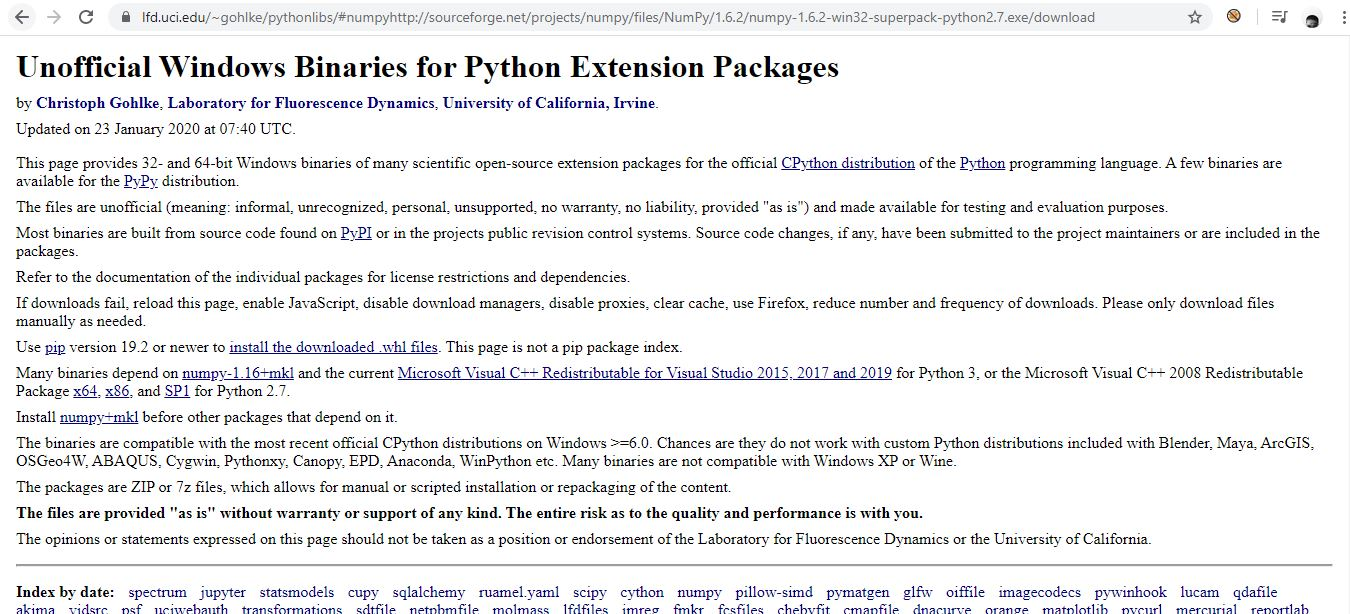
\includegraphics[scale=0.5]{figures/1,2.jpg}
		\caption{Cari SciPy Terbaru pada website ini}
		\label{contoh}
		\end{figure}
	\item Unduh ZIP self-extracting dari OpenCV 3.0.0 dari \begin{verbatim} https://github.com/Itseez/opencv \end{verbatim}. Jalankan ZIP ini, dan ketika diminta, masukkan folder tujuan. 
	\item Salin \begin{verbatim} <unzip_destination>\opencv\build\python\2.7\cv2.pyd \end{verbatim} ke \begin{verbatim} C:\Python2.7\Lib\site-packages \end{verbatim} (dengan asumsi bahwa kami telah menginstal Python 2.7 ke lokasi default). Jika Anda menginstal Python 2.7 dengan Anaconda, gunakan folder instalasi Anaconda daripada instalasi Python default. Sekarang, instalasi Python baru dapat menemukan OpenCV.
	\item Langkah terakhir diperlukan jika kita ingin skrip Python dijalankan menggunakan instalasi Python baru secara default. Edit variabel PATH sistem dan tambahkan C: /Python2.7 (dengan asumsi kami telah menginstal Python 2.7 ke lokasi default) atau folder instalasi Anaconda Anda. Hapus jalur Python sebelumnya, seperti C:/Python2.6. Logout dan login kembali (sebagai alternatif, reboot).
\end{enumerate}

\newpage
\textbf{Menggunakan CMake dan kompiler}

Windows tidak dilengkapi dengan kompiler atau CMake. Kita perlu menginstalnya. Jika kami ingin dukungan untuk kamera kedalaman, termasuk Kinect, kami juga perlu menginstal OpenNI dan SensorKinect.

Mari kita asumsikan bahwa kita telah menginstal Python 2.7, NumPy, dan SciPy 32-bit baik dari binari (seperti dijelaskan sebelumnya) atau dari sumber. Sekarang, kita dapat melanjutkan dengan menginstal kompiler dan CMake, menginstal opsional OpenNI dan SensorKinect, dan kemudian membangun OpenCV dari sumber:

\begin{enumerate}
	\item Unduh dan instal CMake 3.1.2 dari \begin{verbatim} http://www.cmake.org/files/v3.1/cmake3.1.2-win32-x86.exe \end{verbatim} 
		\begin{figure}[ht]
		\centering
		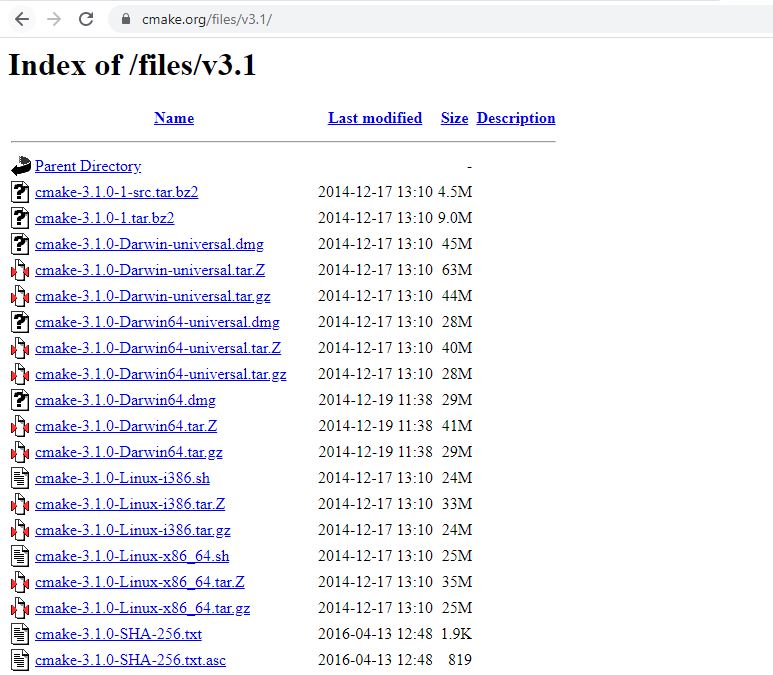
\includegraphics[scale=0.5]{figures/1,3.jpg}
		\caption{Cari CMake Terbaru pada website ini kemudian install}
		\label{contoh}
		\end{figure}
	Saat menjalankan penginstal, pilih Tambahkan CMake ke PATH sistem untuk semua pengguna atau Tambahkan CMake ke PATH sistem untuk pengguna saat ini. Jangan khawatir tentang fakta bahwa CMake versi 64-bit tidak tersedia, CMake hanyalah alat konfigurasi dan tidak melakukan kompilasi apa pun. Sebaliknya, pada Windows, itu menciptakan file proyek yang dapat dibuka dengan Visual Studio.
\newpage
	\item Unduh dan instal Microsoft Visual Studio 2013 (edisi Desktop jika Anda bekerja pada Windows 7) dari \begin{verbatim}https://www.visualstudio.com/products/free-developeroffers-vs.aspx?slcid=0x409&type=web or MinGW \end{verbatim} 
		\begin{figure}[ht]
		\centering
		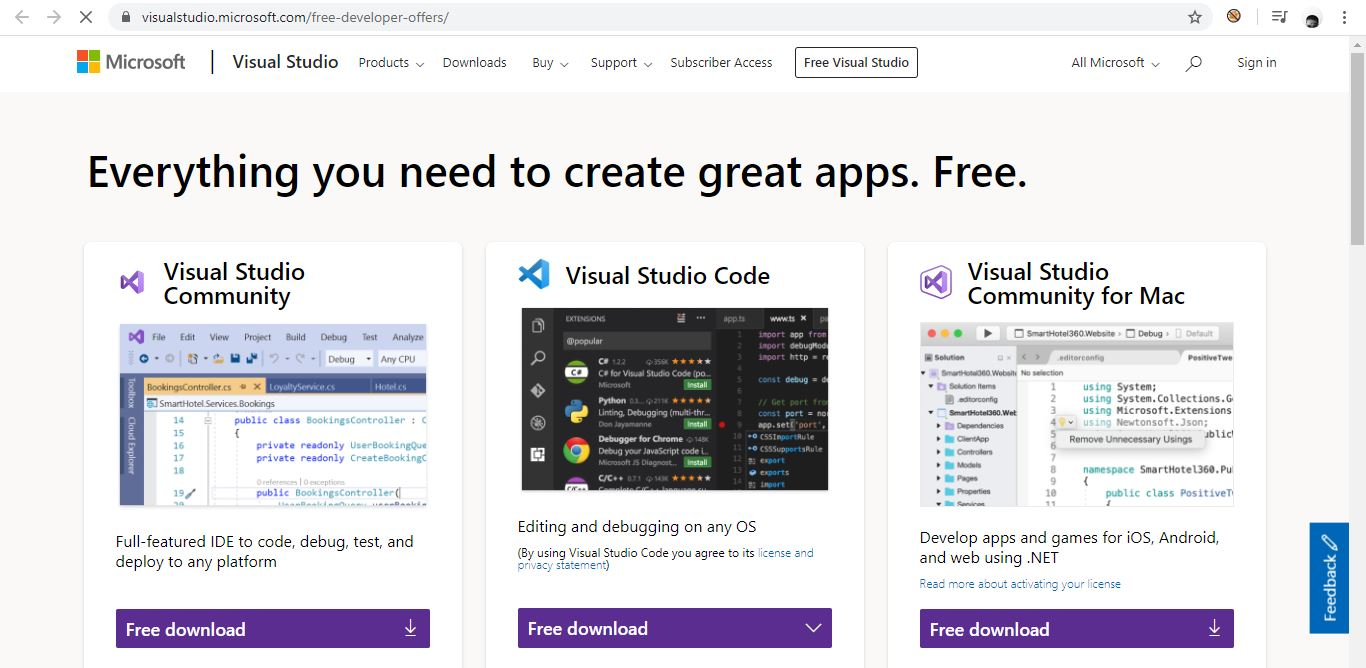
\includegraphics[scale=0.3]{figures/1,4.jpg}
		\caption{Cari VisualStudio Terbaru pada website ini kemudian install}
		\label{contoh}
		\end{figure}
	Perhatikan bahwa Anda harus masuk dengan akun Microsoft Anda dan jika Anda tidak memilikinya, Anda dapat membuatnya di tempat. Instal perangkat lunak dan reboot setelah instalasi selesai. 
\newpage
	\textbf{Untuk MinGW, dapatkan penginstalnya dari} \begin{verbatim}http://sourceforge.net/projects/mingw/files/Installer/mingw-get-setup.exe/download \end{verbatim} 
		\begin{figure}[ht]
		\centering
		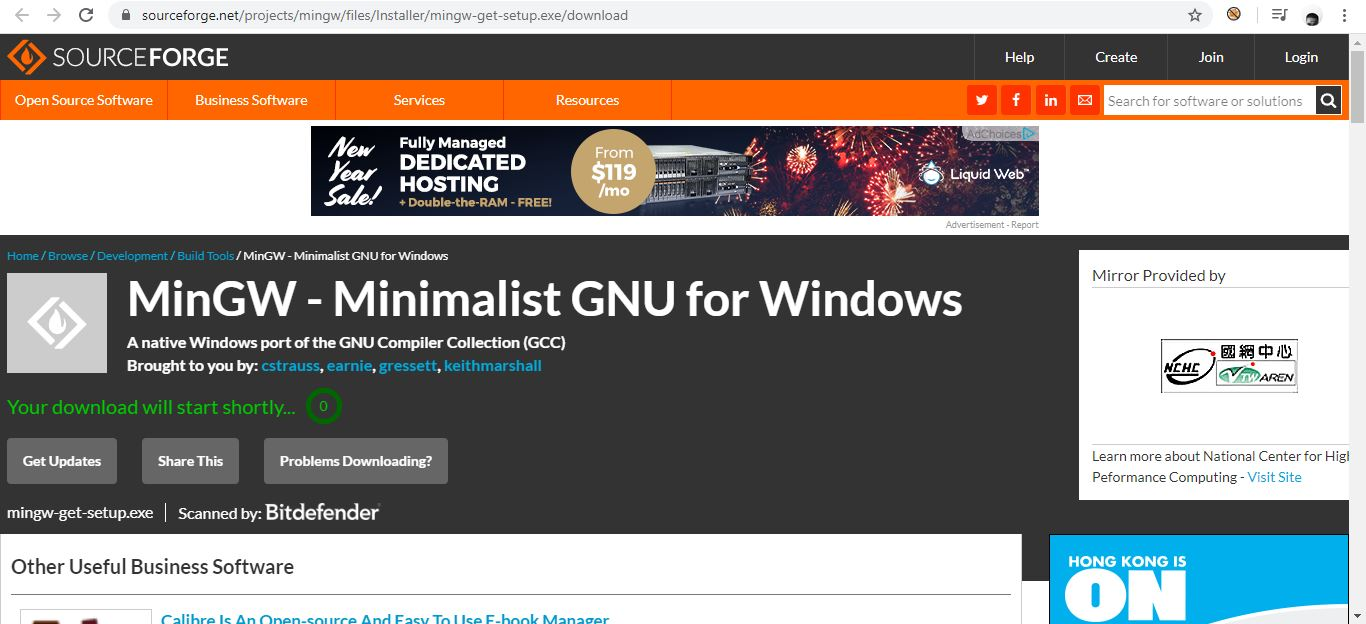
\includegraphics[scale=0.3]{figures/1,5.jpg}
		\caption{Download MinGW}
		\label{contoh}
		\end{figure}
	dan \begin{verbatim}http://sourceforge.net/projects/mingw/files/OldFiles/mingw-get-inst/mingw-getinst-20120426/mingw-get-inst-20120426.exe/download \end{verbatim} 
\newpage
		\begin{figure}[ht]
		\centering
		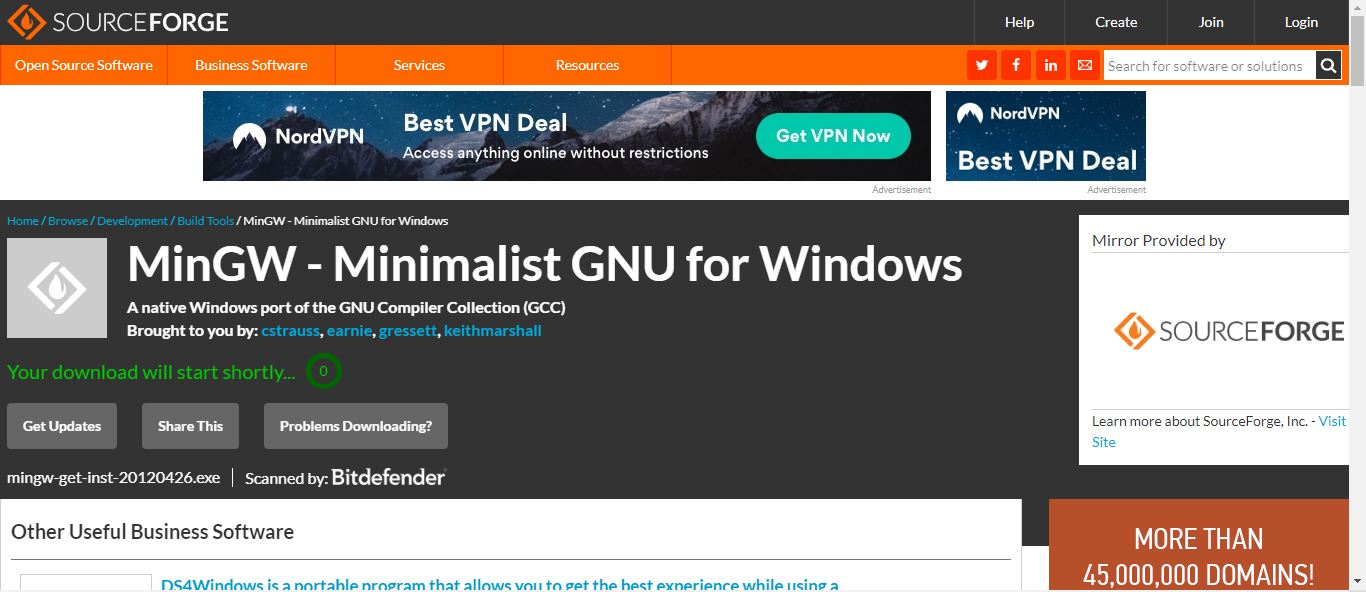
\includegraphics[scale=0.3]{figures/1,6.jpg}
		\caption{Download MinGW}
		\label{contoh}
		\end{figure}
	Saat menjalankan penginstal, pastikan jalur tujuan tidak mengandung spasi dan bahwa kompiler C ++ opsional disertakan. Edit variabel PATH sistem dan tambahkan; \begin{verbatim}C:\MinGW\bin \end{verbatim} (dengan asumsi MinGW diinstal ke lokasi default). Mulai ulang sistem.
	\item Secara opsional, unduh dan instal OpenNI 1.5.4.0 dari tautan yang disediakan di beranda GitHub di OpenNI di \begin{verbatim}https://github.com/OpenNI/OpenNI \end{verbatim}
\newpage
		\begin{figure}[ht]
		\centering
		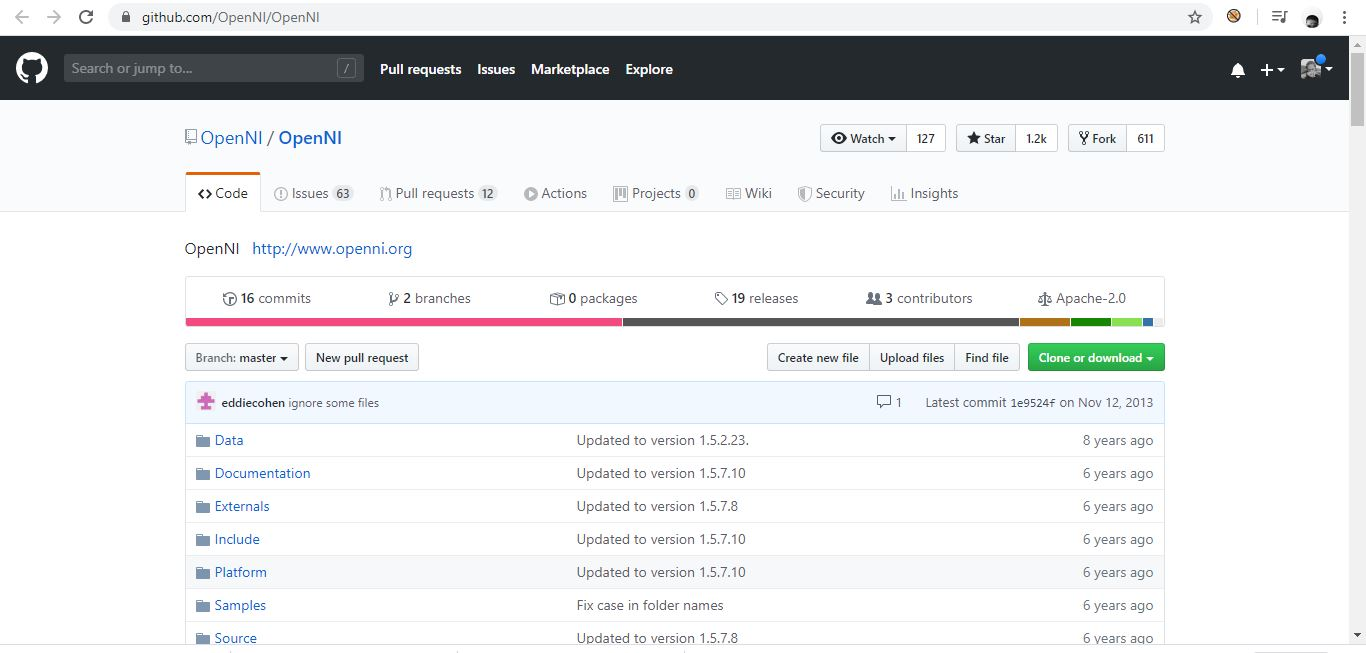
\includegraphics[scale=0.3]{figures/1,7.jpg}
		\caption{Download OpenNI}
		\label{contoh}
		\end{figure}
	\item Anda dapat mengunduh dan menginstal SensorKinect 0.93 dari \begin{verbatim}https://github.com/avin2/SensorKinect/blob/unstable/Bin/SensorKinect093-BinWin32-v5.1.2.1.msi?raw=true (32-bit) \end{verbatim} 
		\begin{figure}[ht]
		\centering
		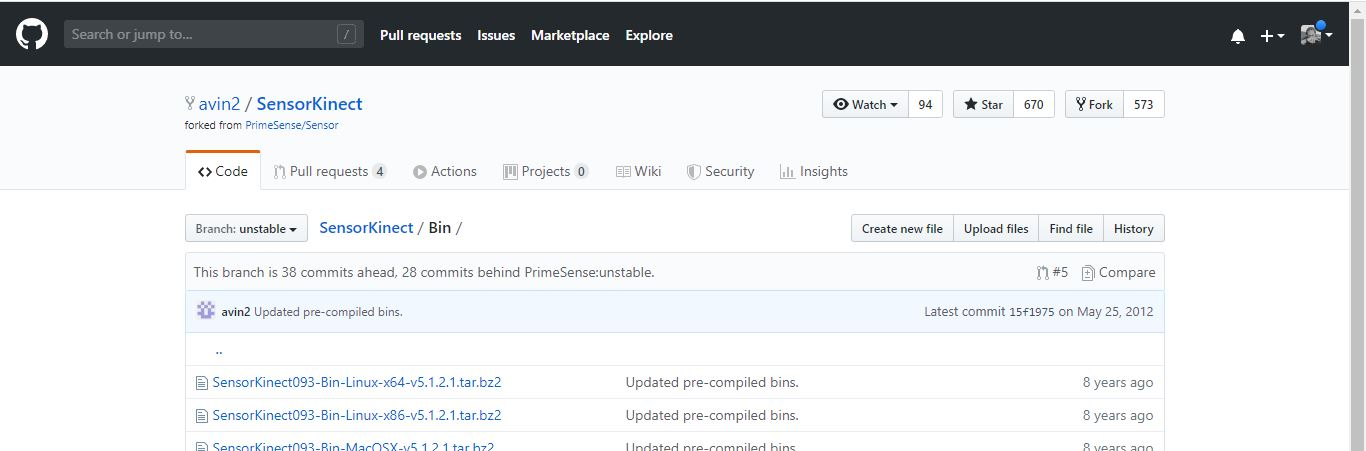
\includegraphics[scale=0.3]{figures/1,8.jpg}
		\caption{Download SensorKinect}
		\label{contoh}
		\end{figure}
\newpage
	Atau, untuk Python 64-bit, unduh di \begin{verbatim} https://github.com/avin2/SensorKinect/blob/unstable/Bin/SensorKinect093-BinWin64-v5.1.2.1.msi?raw=true \end{verbatim}(64-bit). 
		\begin{figure}[ht]
		\centering
		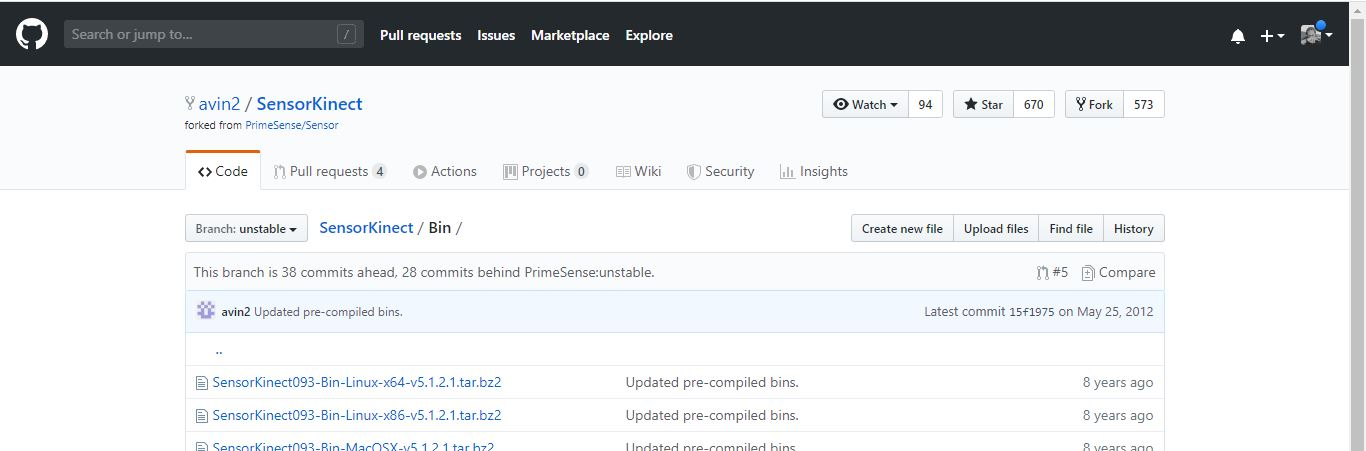
\includegraphics[scale=0.3]{figures/1,8.jpg}
		\caption{Download SensorKinect}
		\label{contoh}
		\end{figure}
	Perhatikan bahwa repositori ini tidak aktif selama lebih dari tiga tahun.
	\item Unduh ZIP self-extracting dari OpenCV 3.0.0 dari \begin{verbatim}https://github.com/Itseez/opencv \end{verbatim} 
		\begin{figure}[ht]
		\centering
		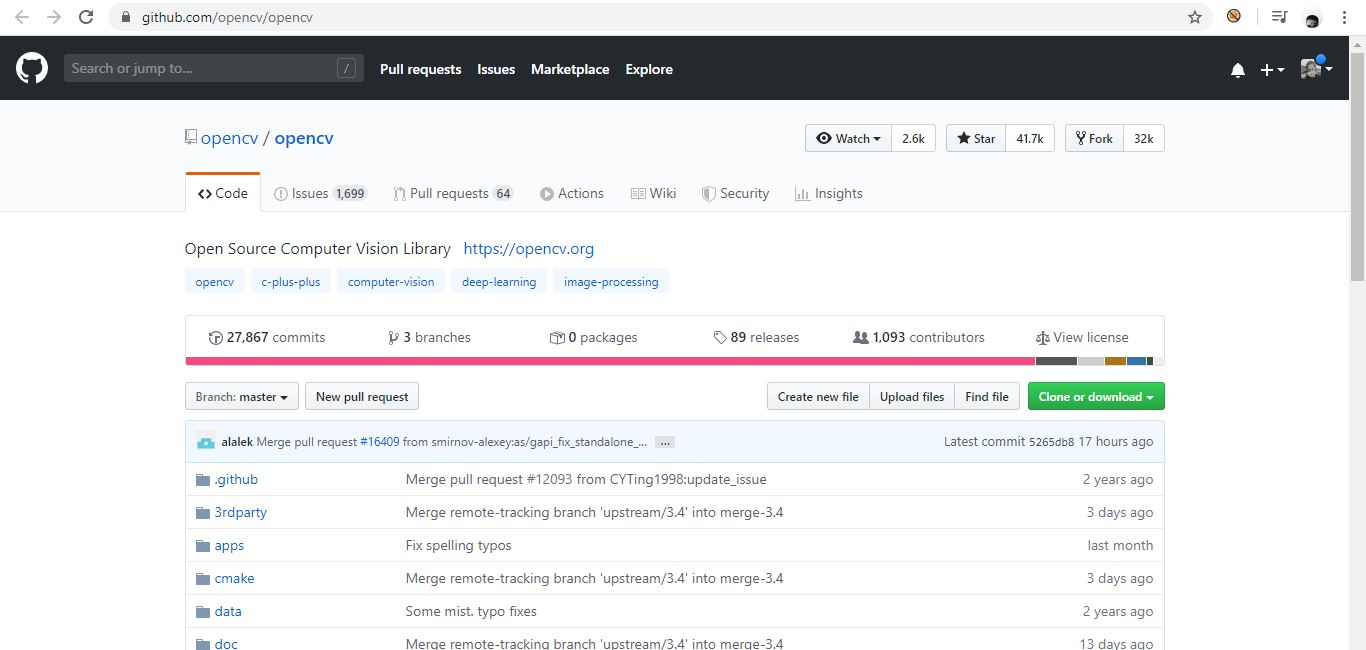
\includegraphics[scale=0.3]{figures/1,9.jpg}
		\caption{Download self-extracting}
		\label{contoh}
		\end{figure}
\newpage
	Jalankan ZIP yang mengekstraksi sendiri, dan ketika diminta, masukkan folder tujuan apa pun, yang akan kita sebut sebagai \begin{verbatim} <unzip_destination>. Subfolder, <unzip_destination>\opencv \end{verbatim} kemudian dibuat.
	\item Buka Command Prompt dan buat folder lain tempat build kita akan menggunakan ini perintah:\begin{verbatim} mkdir <build_folder> Ubah direktori folder build: cd <build_folder> \end{verbatim}
	\item Sekarang, kami siap mengonfigurasi bangunan kami. Untuk memahami semua opsi, kita dapat membaca kode di \begin{verbatim}<unzip_destination>\opencv\CMakeLists.txt \end{verbatim} Namun, untuk tujuan buku ini, kita hanya perlu menggunakan opsi yang akan memberi kita rilis dengan binding Python, dan secara opsional, kedalaman dukungan kamera melalui OpenNI dan SensorKinect.
	\item Buka CMake (cmake-gui) dan tentukan lokasi kode sumber OpenCV dan folder tempat Anda ingin membangun pustaka. Klik pada Konfigurasi. Pilih proyek yang akan dihasilkan. Dalam hal ini, pilih Visual Studio 12 (yang sesuai dengan Visual Studio 2013). Setelah CMake selesai mengkonfigurasi proyek, itu akan menampilkan daftar opsi build. Jika Anda melihat latar belakang merah, itu berarti bahwa proyek Anda mungkin perlu dikonfigurasi ulang: CMake mungkin melaporkan bahwa ia gagal menemukan beberapa dependensi. Banyak dependensi OpenCV adalah opsional, jadi jangan terlalu khawatir. \textbf{Catatan}  Jika build gagal diselesaikan atau Anda mengalami masalah di kemudian hari, coba instal dependensi yang hilang (sering kali tersedia sebagai binari prebuilt), dan kemudian bangun kembali OpenCV dari langkah ini. Anda memiliki opsi untuk memilih / membatalkan pilihan opsi bangunan (sesuai dengan perpustakaan yang telah Anda instal pada mesin Anda) dan klik Konfigurasi lagi, sampai Anda mendapatkan latar belakang yang jelas (putih).
	\item Di akhir proses ini, Anda dapat mengeklik Hasilkan, yang akan membuat file OpenCV.sln di folder yang Anda pilih untuk membangun. Anda kemudian dapat menavigasi ke \begin{verbatim}<build_folder>/OpenCV.sln\end{verbatim} dan membuka file dengan Visual Studio 2013, dan melanjutkan dengan membangun proyek, \begin{verbatim}ALL_BUILD\end{verbatim}. Anda perlu membangun versi Debug dan Rilis dari OpenCV, jadi lanjutkan dan bangun perpustakaan dalam mode Debug, lalu pilih Lepaskan dan bangun kembali (F7 adalah kunci untuk meluncurkan bangunan).
	\item Pada tahap ini, Anda akan memiliki folder bin di direktori build OpenCV, yang akan berisi semua file .dll yang dihasilkan yang memungkinkan Anda untuk memasukkan OpenCV dalam proyek Anda. Atau, untuk MinGW, jalankan perintah berikut:
	\begin{verbatim}
	cmake -D: CMAKE_BUILD_TYPE = RELEASE -D: WITH_OPENNI = ON -G
	"MinGWMakefiles" <unzip_destination>\opencv

	Jika OpenNI tidak diinstal, abaikan -D: WITH_OPENNI = ON. (Dalam hal ini, kamera kedalaman tidak akan didukung.) Jika OpenNI dan SensorKinect diinstal ke lokasi yang tidak cacat, ubah perintah untuk menyertakan -D: OPENNI_LIB_DIR =
	<openni_install_destination>\Lib -D: OPENNI_INCLUDE_DIR =
	<openni_install_destination>\Sertakan -
	D: OPENNI_PRIME_SENSOR_MODULE_BIN_DIR =
	<sensorkinect_install_destination>\Sensor\Bin.

	Atau, untuk MinGW, jalankan perintah ini:

	mingw32-make
	\end{verbatim}
	\item Salin 
	\begin{verbatim}
	<build_folder> \ lib \ Release \ cv2.pyd (dari Visual Studio build) atau
	<build_folder> \ lib \ cv2.pyd (dari build MinGW) hingga
	<python_installation_folder> \ paket-situs.
	\end{verbatim}
	\item Terakhir, edit variabel PATH sistem dan tambahkan
	\begin{verbatim} 
	<build_folder>/bin/Release \end{verbatim}
	(untuk build Visual Studio) atau 
	\begin{verbatim} <build_folder>/bin \end{verbatim}(untuk build MinGW). Mulai ulang sistem anda.

\end{enumerate}
\newpage
\subsection{Instalasi pada OS X}

Beberapa versi Mac digunakan dengan versi Python 2.7 yang sudah diinstal sebelumnya yang disesuaikan oleh Apple untuk kebutuhan internal sistem. Namun, ini telah berubah dan versi standar OS X dikirimkan dengan instalasi standar Python. Di python.org, Anda juga dapat menemukan biner universal yang kompatibel dengan sistem Intel baru dan PowerPC lama.

\textbf{Catatan}

Anda dapat memperoleh penginstal ini di \begin{verbatim} https://www.python.org/downloads/release/python-371/ \end{verbatim} 
		\begin{figure}[ht]
		\centering
		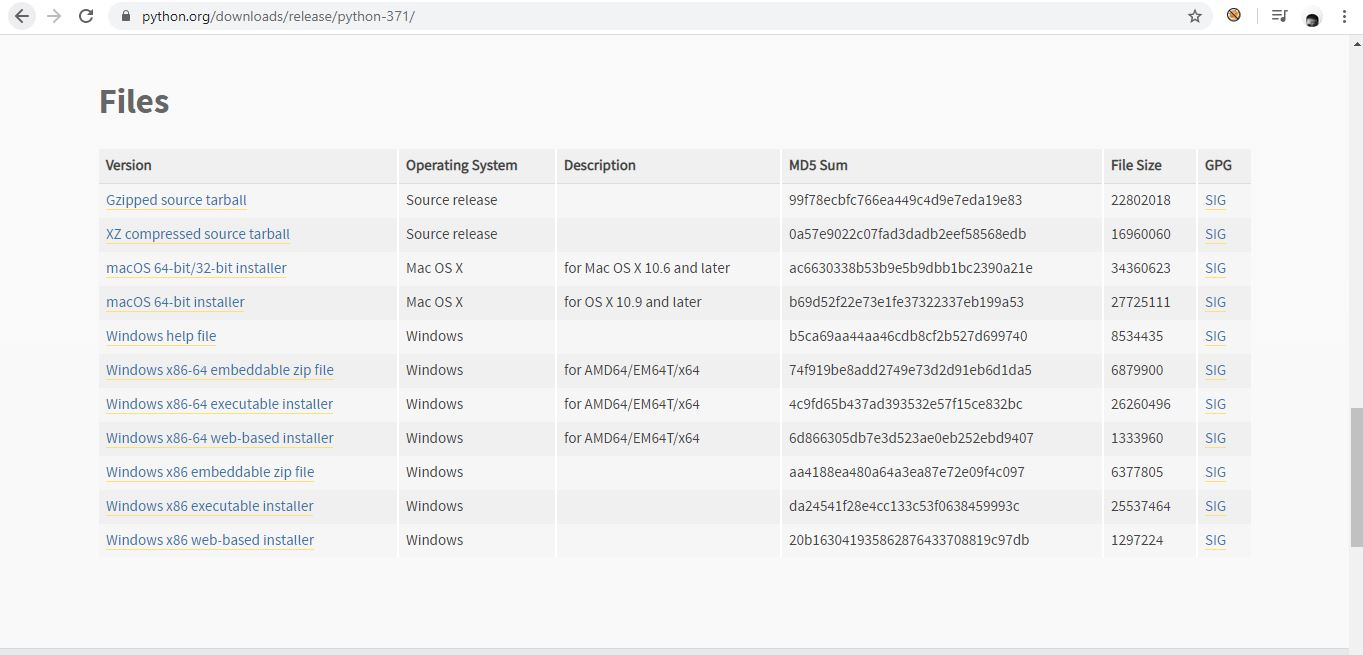
\includegraphics[scale=0.3]{figures/1,10.jpg}
		\caption{Download Python}
		\label{contoh}
		\end{figure}
(lihat PPC Mac OS X 32-bit atau tautan Intel® Mac OS X 64-bit). Menginstal Python dari file .dmg yang diunduh hanya akan menimpa instalasi sistem Python Anda saat ini.

Untuk Mac, ada beberapa pendekatan yang mungkin untuk mendapatkan standar Python 2.7, NumPy, SciPy, dan OpenCV. Semua pendekatan pada akhirnya membutuhkan OpenCV untuk dikompilasi dari sumber menggunakan Alat Pengembang Xcode. Namun, tergantung pada pendekatannya, tugas ini otomatis bagi kami dalam berbagai cara oleh alat pihak ketiga. Kami akan melihat pendekatan semacam ini menggunakan MacPorts atau Homebrew. Alat-alat ini berpotensi melakukan segala yang dapat dilakukan CMake, ditambah lagi membantu kami mengatasi dependensi dan memisahkan pustaka pengembangan kami dari pustaka sistem.
\newpage
\textbf{Tip}

Saya merekomendasikan MacPorts, terutama jika Anda ingin mengkompilasi OpenCV dengan dukungan kamera mendalam melalui OpenNI dan SensorKinect. Tambalan dan skrip yang relevan, termasuk beberapa yang saya kelola, siap pakai untuk MacPorts. Sebaliknya, Homebrew saat ini tidak memberikan solusi yang sudah jadi untuk mengkompilasi OpenCV dengan dukungan kamera yang dalam. Sebelum melanjutkan, pastikan bahwa Alat Pengembang Xcode disiapkan dengan benar:

Unduh dan instal Xcode dari Mac App Store atau \begin{verbatim}https://developer.apple.com/xcode/downloads/ \end{verbatim} Selama instalasi, jika ada opsi untuk menginstal Command Line Tools, pilihlah.

Buka Xcode dan terima perjanjian lisensi.

Langkah terakhir diperlukan jika penginstal tidak memberi kami opsi untuk menginstal Alat Baris Perintah. Arahkan ke Xcode, Preferensi, Unduh, dan klik tombol Instal di sebelah Command Line Tools. Tunggu instalasi untuk menyelesaikan dan keluar dari Xcode.

Atau, Anda dapat menginstal alat baris perintah Xcode dengan menjalankan perintah berikut (di terminal):
\begin{verbatim}
$ xcode-select –install
\end{verbatim}
Sekarang, kami memiliki kompiler yang diperlukan untuk pendekatan apa pun.

Menggunakan MacPorts dengan paket yang sudah jadi

Kita bisa menggunakan manajer paket MacPorts untuk membantu kita mengatur Python 2.7, NumPy, dan OpenCV. MacPorts menyediakan perintah terminal yang mengotomatiskan proses mengunduh, mengkompilasi, dan menginstal berbagai perangkat lunak sumber terbuka (OSS). MacPorts juga menginstal dependensi sesuai kebutuhan. Untuk setiap perangkat lunak, dependensi dan resep bangunan didefinisikan dalam file konfigurasi yang disebut Portfile. Repositori MacPorts adalah kumpulan dari Portfiles.

Mulai dari sistem di mana Xcode dan alat-alat command-line-nya sudah diatur, langkah-langkah berikut akan memberi kita instalasi OpenCV melalui MacPorts:
\newpage
\begin{enumerate}
	\item Unduh dan instal MacPorts dari \begin{verbatim} http://www.macports.org/install.php. \end{verbatim}
		\begin{figure}[ht]
		\centering
		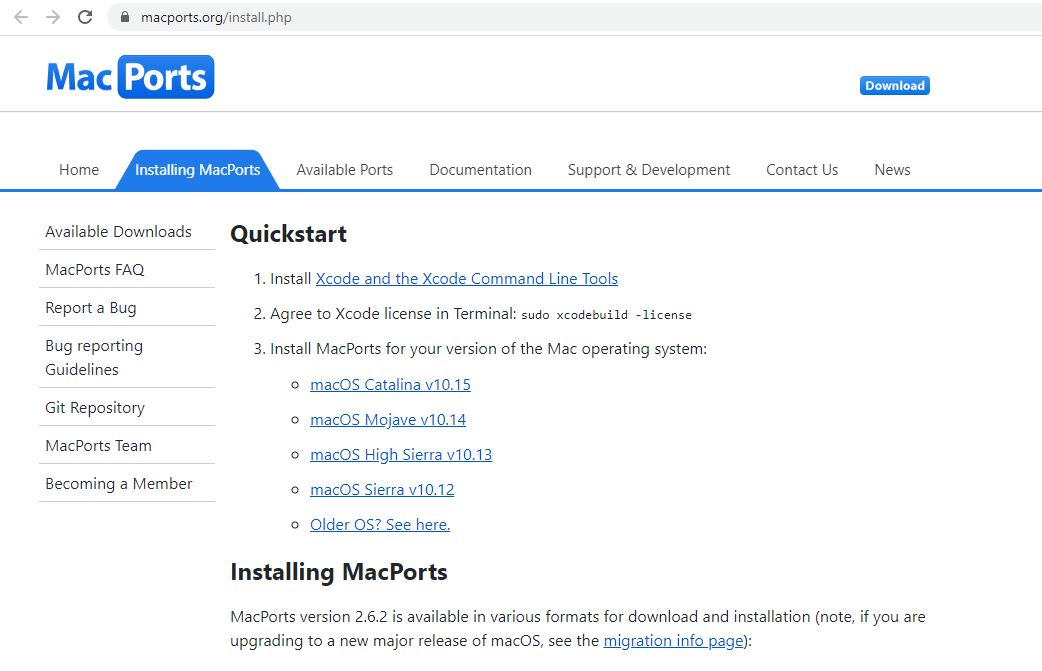
\includegraphics[scale=0.4]{figures/1,11.jpg}
		\caption{Download MacPorts}
		\label{contoh}
		\end{figure}
	\item Jika Anda ingin dukungan untuk kamera kedalaman Kinect, Anda perlu memberi tahu MacPorts tempat untuk mengunduh Portfile khusus yang telah saya tulis. Untuk melakukannya, edit

	/opt/local/etc/macports/sources.conf (dengan asumsi bahwa MacPorts diinstal ke lokasi default). Tepat di atas garis,

	rsync: //rsync.macports.org/release/ports/ [default], tambahkan baris berikut:

	http://nummist.com/opencv/ports.tar.gz

	Simpan file. Sekarang, MacPorts tahu bahwa ia harus mencari Portfile di repositori online saya terlebih dahulu, dan kemudian repositori online default.
	\item Buka terminal dan jalankan perintah berikut untuk memperbarui MacPorts:
	\begin{verbatim}
	$ sudo port selfupdate
	\end{verbatim}
	Saat diminta, masukkan kata sandi Anda.
	\item Sekarang (jika kita menggunakan repositori saya), jalankan perintah berikut untuk menginstal OpenCV dengan binding Python 2.7 dan dukungan untuk kamera kedalaman, termasuk Kinect:
	\begin{verbatim}
	$ sudo port instal opencv + python27 + openni_sensorkinect
	\end{verbatim}
	Atau (dengan atau tanpa repositori saya), jalankan perintah berikut untuk menginstal OpenCV dengan binding Python 2.7 dan dukungan untuk kamera kedalaman, tidak termasuk Kinect:
	\begin{verbatim}
	$ sudo port instal opencv + python27 + openni
	\end{verbatim}

	\textbf{Catatan}

	Ketergantungan, termasuk Python 2.7, NumPy, OpenNI, dan (dalam contoh pertama) SensorKinect, diinstal secara otomatis juga. Dengan menambahkan  python27 ke perintah, kami menentukan bahwa kami ingin varian OpenCV (membangun konfigurasi) dengan Python 2.7 binding. Demikian pula, menambahkan \verb|openni_sensorkinect| menentukan varian dengan dukungan seluas mungkin untuk kamera kedalaman melalui OpenNI dan SensorKinect. Anda dapat menghilangkan \verb|+ openni_sensorkinect| jika Anda tidak bermaksud menggunakan kamera kedalaman, atau Anda dapat menggantinya dengan \verb|+| openni jika Anda bermaksud menggunakan kamera kedalaman yang kompatibel dengan OpenNI tetapi tidak dengan Kinect. Untuk melihat daftar lengkap varian yang tersedia sebelum menginstal, kita dapat memasukkan perintah berikut:
	\begin{verbatim}
	$ port varian opencv
	\end{verbatim}
	Bergantung pada kebutuhan penyesuaian kami, kami dapat menambahkan varian lain ke perintah pemasangan. Untuk fleksibilitas yang lebih besar, kita dapat menulis varian kita sendiri (seperti yang dijelaskan di bagian selanjutnya).
	\item Juga, jalankan perintah berikut untuk menginstal SciPy:
	\begin{verbatim}
	$ sudo port install py27-scipy
	\end{verbatim}
	\item Eksekusi instalasi Python bernama python2.7. Jika kita ingin menautkan python default yang dapat dieksekusi ke python2.7, mari kita juga jalankan perintah ini:
	\begin{verbatim}
	$ sudo port install python_select
	$ sudo port pilih python python27
	\end{verbatim}
\end{enumerate}

\newpage
\textbf{Menggunakan MacPorts dengan paket kustom Anda sendiri}

Dengan beberapa langkah tambahan, kita dapat mengubah cara MacPorts mengkompilasi OpenCV atau perangkat lunak lainnya. Seperti disebutkan sebelumnya, resep build MacPorts didefinisikan dalam file konfigurasi yang disebut Portfiles. Dengan membuat atau mengedit Portfile, kita dapat mengakses alat bantu yang sangat dapat dikonfigurasi, seperti CMake, sementara juga memanfaatkan fitur MacPorts, seperti resolusi ketergantungan.

Mari kita asumsikan bahwa kita sudah menginstal MacPorts. Sekarang, kita dapat mengkonfigurasi MacPorts ke
gunakan Portfile khusus yang kita tulis:

\begin{enumerate}
	\item Buat folder di suatu tempat untuk menampung Portfiles khusus kami. Kami akan merujuk ke folder ini sebagai \begin{verbatim} <local_repository> \end{verbatim}
	\item Edit file /opt/local/etc/macports/sources.conf (dengan anggapan bahwa MacPorts diinstal ke lokasi default). Tepat di atas
	\begin{verbatim} rsync: //rsync.macports.org/release/ports/ default baris, tambahkan baris ini:
	file: // <local_repository>
	Misalnya, jika <local_repository> adalah / Users / Joe / Portfiles, tambahkan baris berikut:
	file: /// Pengguna / Joe / Portfiles \end{verbatim}
	Catat tiga tebasan dan simpan file. Sekarang, MacPorts tahu bahwa ia harus mencari Portfiles di \begin{verbatim} <local_repository> \end{verbatim} terlebih dahulu, dan kemudian, repositori online default-nya.
	\item Buka terminal dan perbarui MacPorts untuk memastikan bahwa kami memiliki Portfile terbaru dari repositori default:
	\begin{verbatim} $ sudo port selfupdate \end{verbatim}
	\item Mari kita salin opencv Portfile repositori default sebagai contoh. Kami juga harus menyalin struktur direktori, yang menentukan bagaimana paket dikategorikan oleh MacPorts:
	\begin{verbatim} $ mkdir <local_repository> / graphics /
	$ cp
	/opt/local/var/macports/sources/rsync.macports.org/release/ports/graphi
	cs / opencv <local_repository> / grafis \end{verbatim}
\newpage
	Sebagai alternatif, untuk contoh yang menyertakan dukungan Kinect, kita dapat mengunduh repositori online saya dari \verb|http://nummist.com/opencv/ports.tar.gz|
		\begin{figure}[ht]
		\centering
		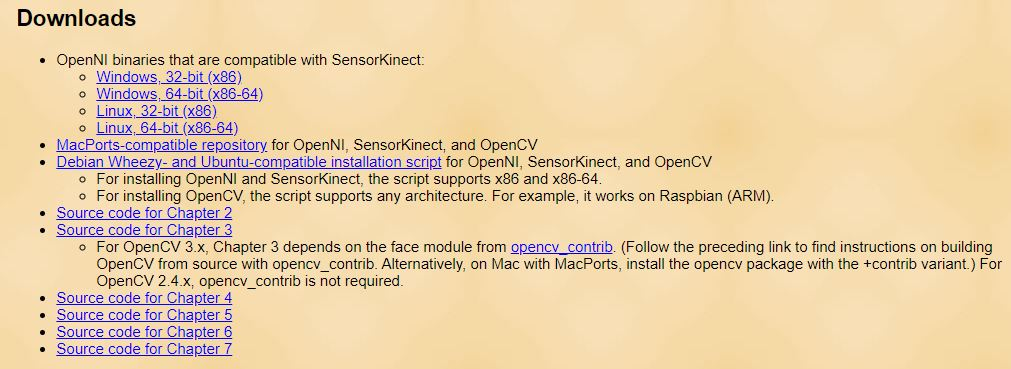
\includegraphics[scale=0.3]{figures/1,12.jpg}
		\caption{Download Kinect}
		\label{contoh}
		\end{figure}
	, unzip, dan salin seluruh folder grafiknya ke \begin{verbatim} <local_repository> \end{verbatim}:
	\begin{verbatim} $ cp <unzip_destination> / graphics <local_repository> \end{verbatim}
	\item Edit \begin{verbatim} <local_repository>/graphics/opencv/Portfile. \end{verbatim} Perhatikan bahwa file ini menentukan flag konfigurasi, dependensi, dan varian CMake. Untuk detail tentang pengeditan Portfile, buka \begin{verbatim} http://guide.macports.org/#development. \end{verbatim}
		\begin{figure}[ht]
		\centering
		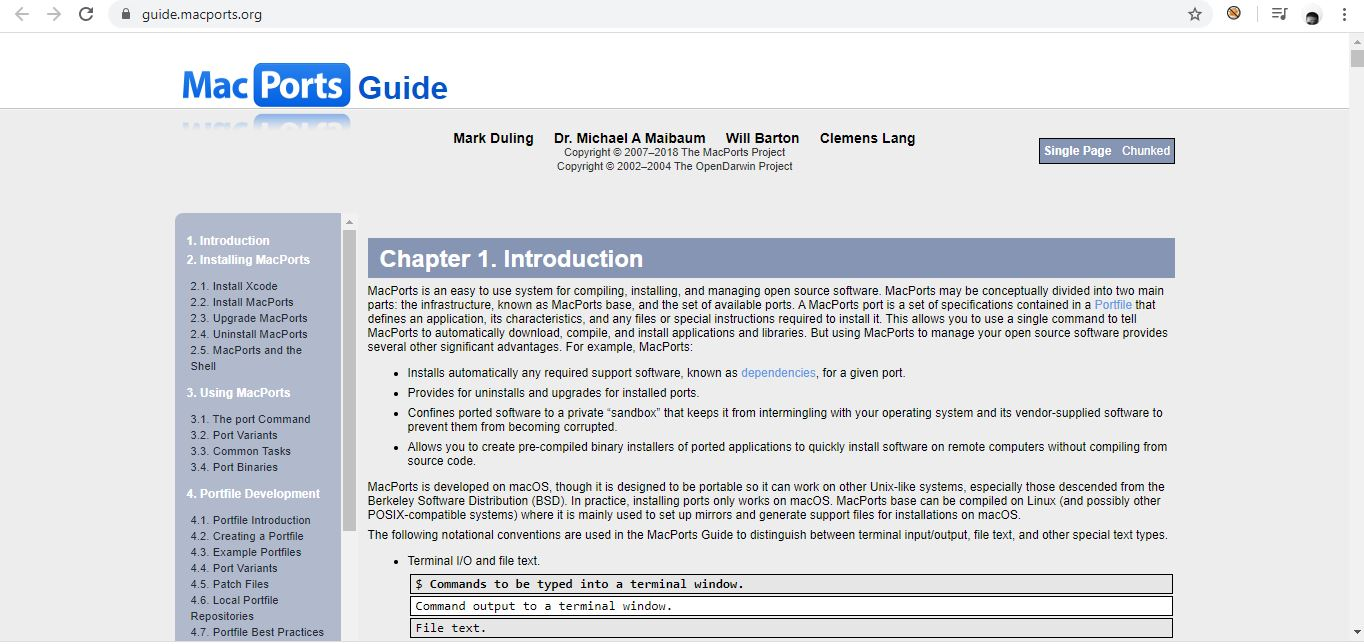
\includegraphics[scale=0.4]{figures/1,13.jpg}
		\caption{Tutorial pada website tersebut}
		\label{contoh}
		\end{figure}
\newpage
	Untuk melihat flag konfigurasi CMake mana yang relevan dengan OpenCV, kita perlu melihat kode sumbernya. Unduh arsip kode sumber dari
	\verb|https://github.com/Itseez/opencv/archive/3.0.0.zip| unzip ke lokasi mana pun, dan baca \verb|<unzip_destination> /OpenCV-3.0.0/CMakeLists.txt.|
	Setelah melakukan pengeditan ke Portfile, simpanlah.
	\item Sekarang, kita perlu membuat file indeks di repositori lokal kita sehingga MacPorts dapat menemukan Portfile baru:
	\begin{verbatim} $ cd <local_repository>
	$ portindex \end{verbatim}
	\item Mulai sekarang, kita dapat memperlakukan file pembuka kustom kita sama seperti paket MacPorts lainnya. Sebagai contoh, kita dapat menginstalnya sebagai berikut:
	\begin{verbatim} $ sudo port instal opencv + python27 + openni_sensorkinect \end{verbatim}
	Perhatikan bahwa Portfile repositori lokal kami lebih diutamakan daripada Portfile repositori default karena urutan urutannya.
	/opt/local/etc/macports/sources.conf.
\end{enumerate}

\newpage
\textbf{Menggunakan Homebrew dengan paket yang sudah jadi (tidak ada dukungan untuk kamera kedalaman)}

Homebrew adalah manajer paket lain yang dapat membantu kami. Biasanya, MacPorts dan Homebrew tidak boleh diinstal pada mesin yang sama. 

Mulai dari sistem di mana Xcode dan alat-alat command-line-nya sudah diatur, langkah-langkah berikut akan memberi kita instalasi OpenCV melalui Homebrew:

\begin{enumerate}
	\item Buka terminal dan jalankan perintah berikut untuk menginstal Homebrew:
	\begin{verbatim}$ ruby ​​-e "$ (curl -fsSkLraw.github.com/mxcl/homebrew/go)" \end{verbatim} 
	\item Tidak seperti MacPorts, Homebrew tidak secara otomatis menempatkan executable-nya di PATH. Untuk melakukannya, buat atau edit file \begin{verbatim} ~/.profile \end{verbatim} dan tambahkan baris ini di bagian atas kode:
	\begin{verbatim} 
	eksport PATH = / usr / local / bin: / usr / local / sbin: $ PATH
	\end{verbatim}
	Simpan file dan jalankan perintah ini untuk menyegarkan PATH:
	\begin{verbatim} 
	$ source ~/.profile
	\end{verbatim}
	Perhatikan bahwa executable yang diinstal oleh Homebrew sekarang diutamakan daripada executable yang diinstal oleh sistem.

	\item Untuk laporan diagnostik mandiri Homebrew, jalankan perintah berikut:
	\begin{verbatim} 
	$ brew doctor
	\end{verbatim}
	Ikuti saran pemecahan masalah yang diberikannya.
	\item Sekarang, perbarui Homebrew:
	\begin{verbatim} 
	$ brew update
	\end{verbatim}
	\item Jalankan perintah berikut untuk menginstal Python 2.7:
	\begin{verbatim} 
	$ brew install python
	\end{verbatim}	
	\item Sekarang, kita dapat menginstal NumPy. Pilihan paket pustaka Python Homebrew terbatas, jadi kami menggunakan alat manajemen paket terpisah yang disebut pip, yang dilengkapi dengan Homebrew Python:
	\begin{verbatim} 
	$ pip install numpy
	\end{verbatim}
	\item SciPy berisi beberapa kode Fortran, jadi kita memerlukan kompiler yang sesuai. Kita dapat menggunakan Homebrew untuk menginstal kompiler gfortran:
	\begin{verbatim} 
	$ brew install gfortran
	\end{verbatim}
	Sekarang, kita dapat menginstal SciPy:
	\begin{verbatim} 
	$ pip install scipy
	\end{verbatim}
	\item Untuk menginstal OpenCV pada sistem 64-bit (semua perangkat keras Mac baru sejak akhir 2006), jalankan
	perintah berikut:
	
\begin{enumerate}

\newpage
\textbf{Tip}
\newline
\textbf{Mengunduh kode contoh}
\newline

Anda dapat mengunduh file kode contoh untuk semua buku Penerbitan Packt yang telah Anda beli dari akun Anda di \begin{verbatim} http://www.packtpub.com.\end{verbatim} Jika Anda membeli buku ini di tempat lain, Anda dapat mengunjungi \begin{verbatim} http://www.packtpub.com/support\end{verbatim} dan mendaftar agar file-file tersebut diemail langsung kepada Anda.
		\begin{figure}[ht]
		\centering
		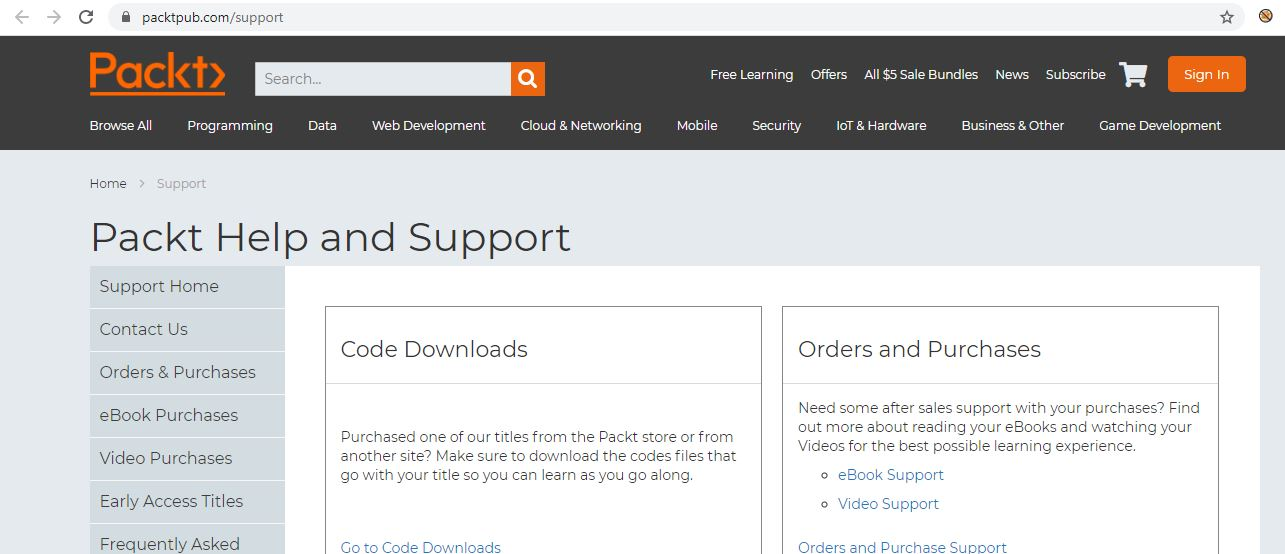
\includegraphics[scale=0.4]{figures/1,14.jpg}
		\caption{Website packtpub}
		\label{contoh}
		\end{figure}

\textbf{Menggunakan Homebrew dengan paket kustom Anda sendiri}
\newline
Homebrew memudahkan untuk mengedit definisi paket yang ada:
\begin{verbatim} 
$ brew edit opencv
\end{verbatim}

Definisi paket sebenarnya adalah skrip dalam bahasa pemrograman Ruby. Kiat untuk mengeditnya dapat ditemukan di halaman Wiki Homebrew di \begin{verbatim} https://github.com/mxcl/homebrew/wiki/Formula-Cookbook. \end{verbatim} Sebuah skrip dapat menentukan flag konfigurasi Make atau CMake, antara lain.

Untuk melihat flag konfigurasi CMake mana yang relevan dengan OpenCV, kita perlu melihat kode sumbernya. Unduh arsip kode sumber dari \begin{verbatim} https://github.com/Itseez/opencv/archive/3.0.0.zip \end{verbatim}, unzip ke lokasi mana pun, dan baca \begin{verbatim} <unzip_destination>/OpenCV-2.4.3/CMakeLists.txt. \end{verbatim}
Setelah mengedit skrip Ruby, simpan.
Paket khusus dapat diperlakukan seperti biasa. Misalnya, dapat diinstal sebagai berikut:
\begin{verbatim} 
$ brew install opencv
\end{verbatim}


\newpage
\subsection {Instalasi pada Ubuntu}

Pertama dan terpenting, berikut adalah catatan singkat tentang versi Ubuntu dari sistem operasi: Ubuntu memiliki siklus rilis 6 bulan di mana setiap rilis adalah versi minor .04 atau .10 dari versi utama (14 pada saat penulisan). Namun, setiap dua tahun, Ubuntu merilis versi yang diklasifikasikan sebagai dukungan jangka panjang (LTS) yang akan memberi Anda dukungan lima tahun oleh Canonical (perusahaan di belakang Ubuntu). Jika Anda bekerja di lingkungan perusahaan, disarankan untuk menginstal salah satu versi LTS. Yang terbaru yang tersedia adalah 14,04.


Ubuntu hadir dengan Python 2.7 yang sudah diinstal. Repositori Ubuntu standar berisi paket OpenCV 2.4.9 tanpa dukungan untuk kamera yang dalam. Pada saat penulisan ini, OpenCV 3 belum tersedia melalui repositori Ubuntu, jadi kita harus membuatnya dari sumber. Untungnya, sebagian besar sistem Unix-like dan Linux datang dengan semua perangkat lunak yang diperlukan untuk membangun proyek dari awal yang sudah diinstal. Ketika dibangun dari sumber, OpenCV dapat mendukung kamera kedalaman melalui OpenNI dan SensorKinect, yang tersedia sebagai binari yang dikompilasi dengan skrip instalasi.

\par
\textbf {Menggunakan repositori Ubuntu (tidak ada dukungan untuk kamera kedalaman)}

Kita dapat menginstal Python dan semua dependensi yang diperlukan menggunakan manajer paket apt, dengan menjalankan perintah berikut:
\begin{verbatim}
> sudo apt-get install build-essential
> sudo apt-get install cmake git libgtk2.0-dev pkg-config libavcodecdev
libavformat-dev libswscale-dev
> sudo apt-get install python-dev python-numpy libtbb2 libtbb-dev libjpegdev libpng-dev libtiff-dev libjasper-dev libdc1394-22-dev 
\end{verbatim}
Secara setara, kita bisa menggunakan Ubuntu Software Center, yang merupakan tampilan grafis apt package manager.

\newpage
\textbf {Membangun OpenCV dari sumber}
Sekarang kita telah menginstal seluruh tumpukan Python dan cmake, kita dapat membangun OpenCV.
Pertama, kita perlu mengunduh kode sumbernya
\verb| https: //github.com/Itseez/opencv/archive/3.0.0-beta.zip. |
Ekstrak arsip dan pindahkan ke folder yang tidak di-zip di terminal.
Kemudian, jalankan perintah berikut:
\begin{verbatim}
> mkdir build
> cd build
> cmake -D CMAKE_BUILD_TYPE =Release -D CMAKE_INSTALL_PREFIX =/usr/local ..
> make
> make install 
\end{verbatim}

Setelah instalasi berakhir, Anda mungkin ingin melihat contoh Python OpenCV di
\verb|<opencv_folder>/opencv/samples/python| dan
\verb|<script_folder>/opencv/samples/python2.|

Instalasi pada sistem mirip Unix lainnya
Pendekatan untuk Ubuntu (seperti yang dijelaskan sebelumnya) kemungkinan akan bekerja pada distribusi Linux apa pun yang berasal dari Ubuntu 14.04 LTS atau Ubuntu 14.10 sebagai berikut:
Kubuntu 14.04 LTS atau Kubuntu 14.10
Xubuntu 14.04 LTS atau Xubuntu 14.10
Linux Mint 17

Pada Debian Linux dan turunannya, manajer paket apt berfungsi sama seperti di Ubuntu, meskipun paket yang tersedia mungkin berbeda.

Di Gentoo Linux dan turunannya, manajer paket Portage mirip dengan MacPorts (seperti dijelaskan sebelumnya), meskipun paket yang tersedia mungkin berbeda.

Pada turunan FreeBSD, proses instalasi sekali lagi mirip dengan MacPorts; sebenarnya, MacPorts berasal dari sistem instalasi port yang diadopsi pada FreeBSD. Bacalah Buku Pegangan FreeBSD yang luar biasa di \newline \verb|https://www.freebsd.org/doc/handbook/| untuk ikhtisar proses instalasi perangkat lunak.
		\begin{figure}[ht]
		\centering
		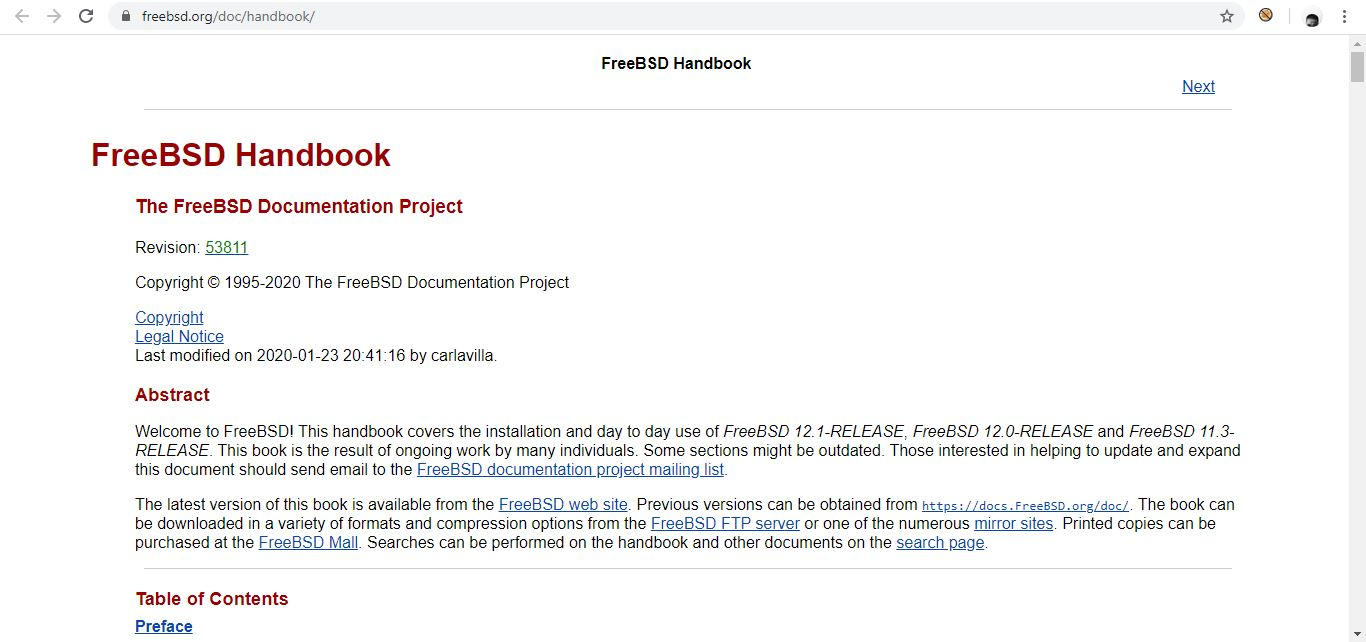
\includegraphics[scale=0.4]{figures/1,15.jpg}
		\caption{FreeBSD}
		\label{contoh}
		\end{figure}
\newpage
Pada sistem mirip Unix lainnya, manajer paket dan paket yang tersedia mungkin berbeda. Konsultasikan dokumentasi manajer paket Anda dan cari paket dengan opencv di namanya. Ingatlah bahwa OpenCV dan binding Python-nya dapat dipecah menjadi beberapa
paket.

Juga, cari semua catatan instalasi yang diterbitkan oleh penyedia sistem, pengelola repositori, atau komunitas. Karena OpenCV menggunakan driver kamera dan codec media, membuat semua fungsinya berfungsi dapat menjadi rumit pada sistem dengan dukungan multimedia yang buruk. Dalam beberapa keadaan, paket sistem mungkin perlu dikonfigurasi ulang atau diinstal ulang untuk kompatibilitas.

Jika paket tersedia untuk OpenCV, periksa nomor versinya. OpenCV 3 atau lebih tinggi direkomendasikan untuk tujuan buku ini. Juga, periksa apakah paket menawarkan binding Python dan dukungan kamera mendalam melalui OpenNI dan SensorKinect. Terakhir, periksa apakah ada orang di komunitas pengembang yang melaporkan keberhasilan atau kegagalan dalam menggunakan paket.

Jika, sebaliknya, kami ingin melakukan pembuatan kustom OpenCV dari sumber, mungkin bermanfaat untuk merujuk ke skrip instalasi untuk Ubuntu (seperti yang dibahas sebelumnya) dan menyesuaikannya dengan manajer paket dan paket yang ada di sistem lain.


\newpage
\subsection {Instalasi modul Contrib}
Berbeda dengan OpenCV 2.4, beberapa modul terdapat dalam repositori yang disebut \verb|opencv_contrib|, yang tersedia di \verb|https://github.com/Itseez/opencv_contrib.| Saya sangat merekomendasikan menginstal modul ini karena mengandung fungsionalitas tambahan yang tidak termasuk dalam OpenCV, seperti modul pengenalan wajah.
Setelah diunduh (baik melalui zip atau git, saya sarankan git agar Anda dapat tetap up to date dengan perintah git pull sederhana), Anda dapat menjalankan kembali perintah cmake Anda untuk memasukkan pembangunan OpenCV dengan modul \verb|opencv_contrib| sebagai berikut:
\begin{verbatim}
cmake -DOPENCV_EXTRA_MODULES_PATH = <opencv_contrib> / modules
<opencv_source_directory>
\end{verbatim}

Jadi, jika Anda telah mengikuti prosedur standar dan membuat direktori build di folder unduhan OpenCV Anda, Anda harus menjalankan perintah berikut:

\begin{verbatim}
mkdir build && cd build
cmake -D CMAKE_BUILD_TYPE = Lepaskan -DOPENCV_EXTRA_MODULES_PATH =
<opencv_contrib> / modules -D CMAKE_INSTALL_PREFIX = / usr / local ..
make
\end{verbatim}

\newpage
\subsection {PyCharm}
Pycharm merupakan tools untuk menjalankan program python didalamnya sudah terdapat berbagai macam library dari python itu sendiri, kita hanya perlu mencari library yang kita butuhkan kemudian klik install, maka kita tidak perlu melakukan hal hal yang telah di contohkan untuk menginstall opencv pada windows atau yang lainnya. Yang perlu kita lakukan yang pertama kalinya adalah kita mendownload aplikasi PyCharm. \newline \verb|https://www.jetbrains.com/pycharm/download/#section=windows| \newline 
		\begin{figure}[ht]
		\centering
		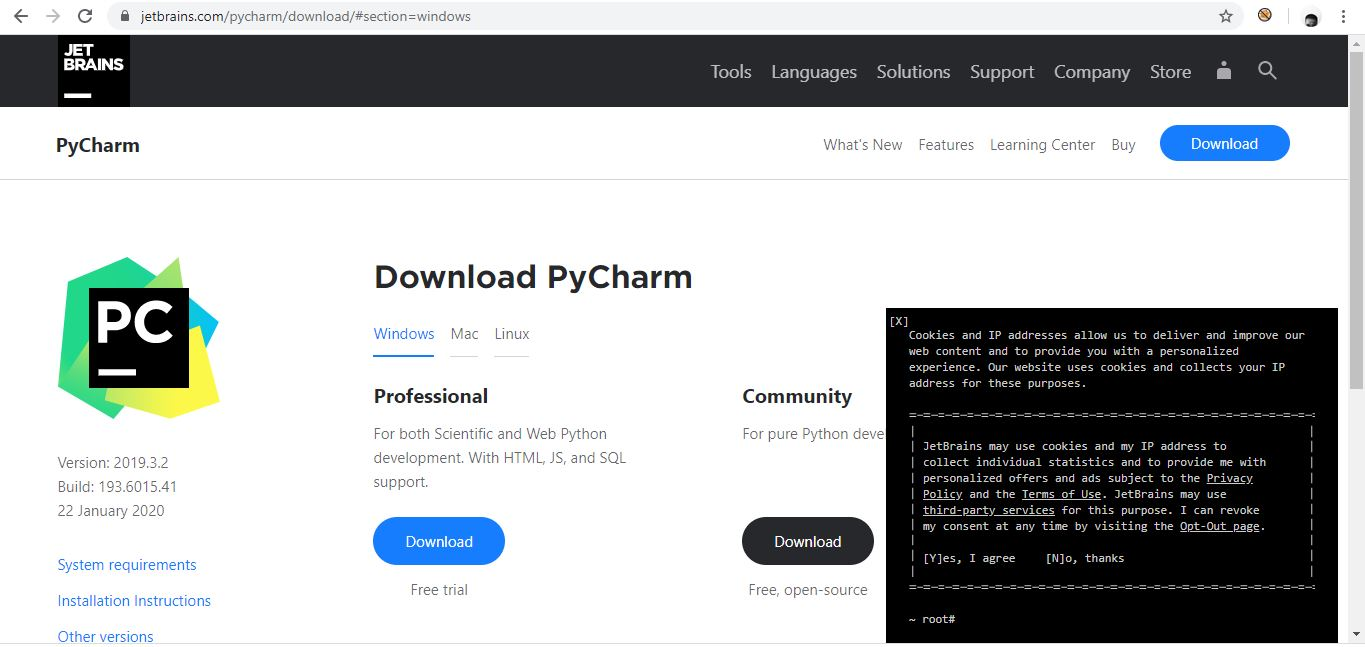
\includegraphics[scale=0.4]{figures/1,16.jpg}
		\caption{Pycharm}
		\label{contoh}
		\end{figure}
\newpage
Kemudian lakukan installasi, setelah istallasi selesai selanjutnya kita buka aplikasi kemudian pilih file kemudian settings.
		\begin{figure}[ht]
		\centering
		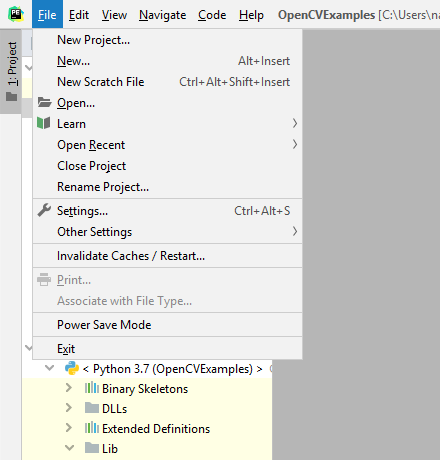
\includegraphics[scale=0.4]{figures/1,17.png}
		\caption{Pycharm Settings}
		\label{contoh}
		\end{figure}
\newline
Kemudian pilih project interpreter, lalu klik tambah pada pojok kanan, maka tampilannya akan seperti ini:
		\begin{figure}[ht]
		\centering
		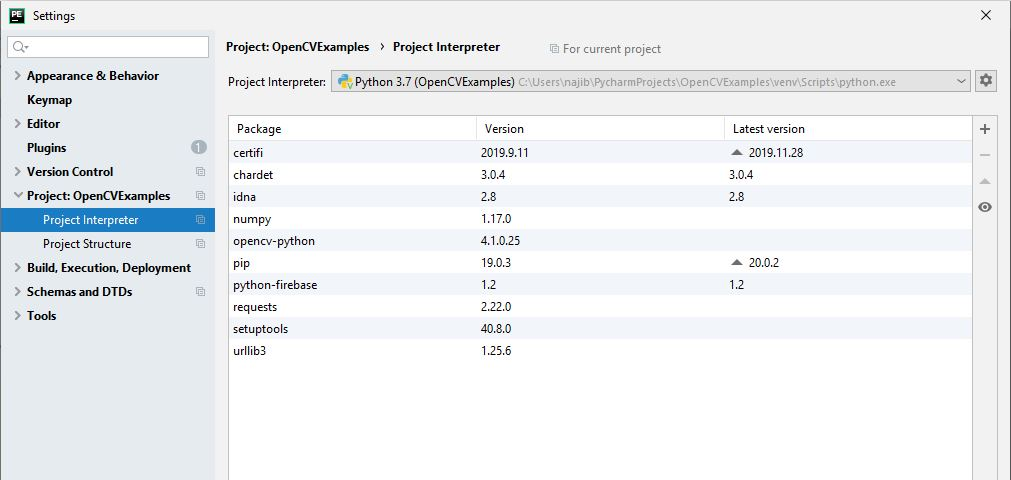
\includegraphics[scale=0.4]{figures/1,18.jpg}
		\caption{Install library}
		\label{contoh}
		\end{figure}
\newpage
Setelah masuk pada tampilan ini kita cari library apa yang kita butuhkan untuk menjalankan project yang akan kita bangun, karna bahasan kita pada saat ini yaitu OPENCV maka yang kita cari adalah OpenCV, Setelah menemukannya kita langsung saja klik install kira kira membutuhkan waktu lumayan lama, jika internet kita stabil kurang lebih 20-30 menit waktu yang di butuhkan untuk menginstall opencv ini.
		\begin{figure}[ht]
		\centering
		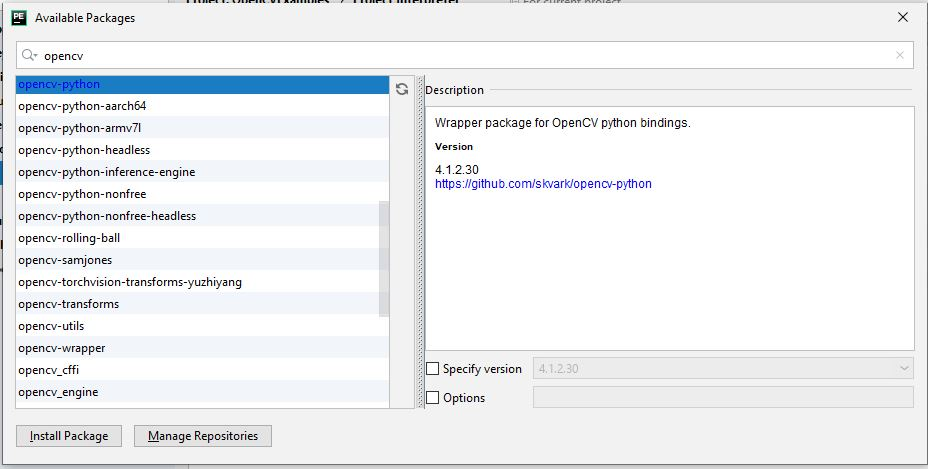
\includegraphics[scale=0.4]{figures/1,19.jpg}
		\caption{Install OpenCV}
		\label{contoh}
		\end{figure}
%\chapter{Dasar Dasar Code OpenCV}
\section{Menampilkan gambar}
\subsection{Menampilkan Gambar}

\lstinputlisting{src/cv2.py}
\begin{enumerate}
	\item lakukan Import library open cv yaitu cv2
	\item kemudian panggil file foto menggunakan kode seperti di atas, membuat terlebihdahulu variabel img, kemudian cv2.imread nama file dan nomor untuk gradiasi warnanya, pada bagian ini menggunakan angka 1 yang artinya mengikuti foto aslinya.
	\item lakukan print untuk menampilkan gambar
	\item kemudian buat frame untuk menampilkan gambar menggunakan imshow dengan nama frame image.
	\item kemudian gunakan waitKey untuk membuat frame agar tidak langsung mati atau tertutup otomatis.
	\item destroyAllWindows digunakan untuk menutup frame.
\end{enumerate}

\begin{figure}[ht]
\centering
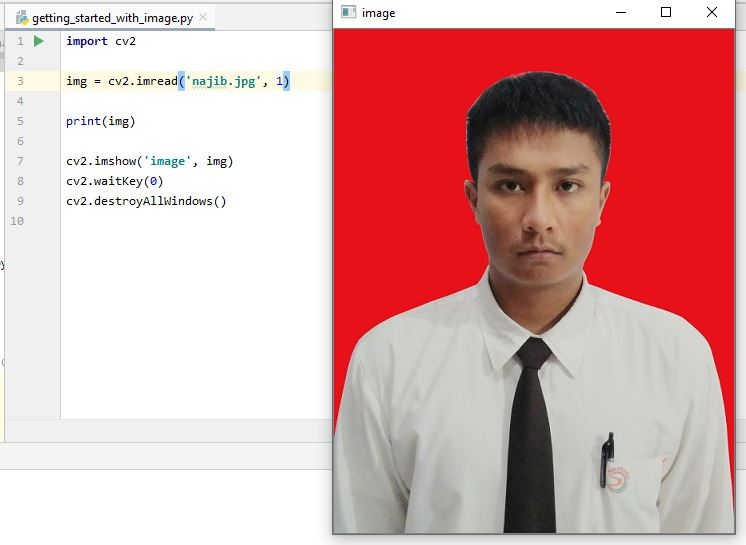
\includegraphics[scale=0.5]{figures/2,2.jpg}
\caption{Menampilkan gambar}
\label{contoh}
\end{figure}
Hasil yang ditampilkan sama seperti foto aslinya karna tidak ada dari foto yang di rubah sama sekali, kodingan ini hanya bertujuan untuk menampilkan gambar saja.

\newpage
\subsection{Menampilkan Gambar dan merubah kontras warnanya}
\lstinputlisting{src/cv1.py}
\begin{enumerate}
	\item lakukan Import library open cv yaitu cv2
	\item kemudian panggil file foto menggunakan kode seperti di atas, membuat terlebihdahulu variabel img, kemudian cv2.imread nama file dan nomor untuk gradiasi warnanya, pada bagian ini menggunakan angka 0 merubah gambar menjadi hitam putih.
	\item lakukan print untuk menampilkan gambar
	\item kemudian buat frame untuk menampilkan gambar menggunakan imshow dengan nama frame image.
	\item kemudian gunakan waitKey untuk membuat frame agar tidak langsung mati atau tertutup otomatis.
	\item destroyAllWindows digunakan untuk menutup frame.
\end{enumerate}


\begin{figure}[ht]
\centering
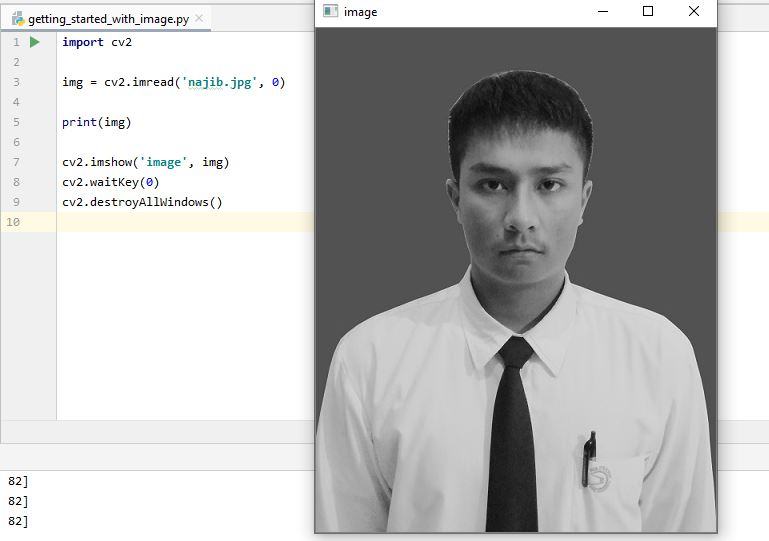
\includegraphics[scale=0.5]{figures/2,1.jpg}
\caption{Merubah kontras warna}
\label{contoh}
\end{figure}

Pada bagian kodingan ini foto di rubah kontras warnanya menjadi hitam putih, pada kodingan sebelumnya yang di rubah hanya satu huruf saja untu menjadikan foto ini menjadi seperti ini. yaitu pada bagian imread nya menjadi 0.

\subsection{Menyimpan Gambar menggunakan kode opencv}
\lstinputlisting{src/cv3.py}
\begin{enumerate}
	\item lakukan Import library open cv yaitu cv2
	\item kemudian panggil file foto menggunakan kode seperti di atas, membuat terlebihdahulu variabel img, kemudian cv2.imread nama file dan nomor untuk gradiasi warnanya, pada bagian ini menggunakan angka 0 merubah gambar menjadi hitam putih.
	\item lakukan print untuk menampilkan gambar
	\item kemudian buat frame untuk menampilkan gambar menggunakan imshow dengan nama frame image.
	\item kemudian gunakan waitKey untuk membuat frame agar tidak langsung mati atau tertutup otomatis.
	\item destroyAllWindows digunakan untuk menutup frame.
	\item terakhir gambar disimpan menggunakan kode imwrite, pertama tuliskan nama gambar yang akan disimpan beserta formatgambarnya, kemudian kode img untuk menyatakan yang disimpan tersebut adalah gambar.
\end{enumerate}

\newpage
\begin{figure}[ht]
\centering
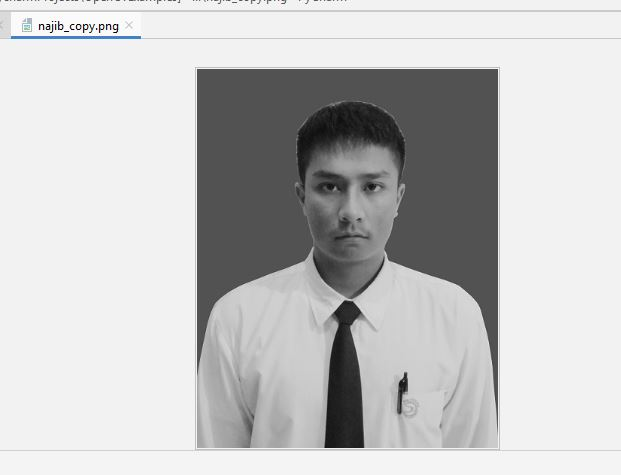
\includegraphics[scale=0.5]{figures/2,3.jpg}
\caption{Menyimpan gambar}
\label{contoh}
\end{figure}

Gambar berhasil disimpan dengan nama najibcopy.png, gambar disimpan sesuai yang telah di edit kontras warnanya menjadi hitam putih sesuai cede yang kita jalankan.

\newpage
\section{Menjalankan kamera leptop}
\subsection{Menjalankan video kamera leptop}
\lstinputlisting{src/cv4.py}
\begin{enumerate}
	\item lakukan Import library open cv yaitu cv2
	\item kemudian buat variable baru dengan nama cap kemudian panggil VideoCapture(0) yang artinya menjalankan kamera leptop.
	\item membuat while yaitu perulangan membuka frame
	\item kemudian didalam perulangan tersebut terdapat frame yang membaca atau merekam video.
	\item kemudian buat frame dengan nama frame
	\item kemudian gunakan waitKey untuk membuat frame agar tidak langsung mati atau tertutup otomatis.
	\item release untuk menutup videocapture
	\item destroyAllWindows digunakan untuk menutup frame.
\end{enumerate}

\newpage
\begin{figure}[ht]
\centering
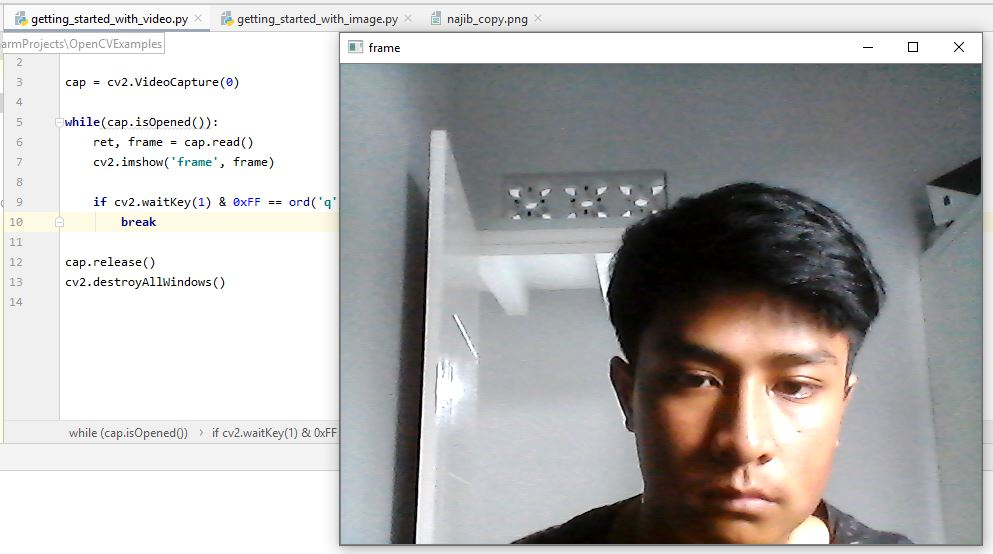
\includegraphics[scale=0.5]{figures/2,4.jpg}
\caption{Menggunakan kamera leptop}
\label{contoh}
\end{figure}

Pada videocpture ini hanya merekam menggunakan kamera leptop saja belum masuk ke pengolahan gambar.

\newpage
\subsection{Merubah kontras warna pada video}
\lstinputlisting{src/cv5.py}
\begin{enumerate}
	\item lakukan Import library open cv yaitu cv2
	\item kemudian buat variable baru dengan nama cap kemudian panggil VideoCapture(0) yang artinya menjalankan kamera leptop.
	\item membuat while yaitu perulangan membuka frame
	\item kemudian didalam perulangan tersebut terdapat frame yang membaca atau merekam video.
	\item buat variable dengan nama gray karna kita mau berubah kontras warnanya menjadi hitam putih, kemudian panggil cvtColor didalam frame dengan warna abu abu.
	\item kemudian buat frame dengan nama frame
	\item kemudian gunakan waitKey untuk membuat frame agar tidak langsung mati atau tertutup otomatis.
	\item release untuk menutup videocapture
	\item destroyAllWindows digunakan untuk menutup frame.
\end{enumerate}

\begin{figure}[ht]
\centering
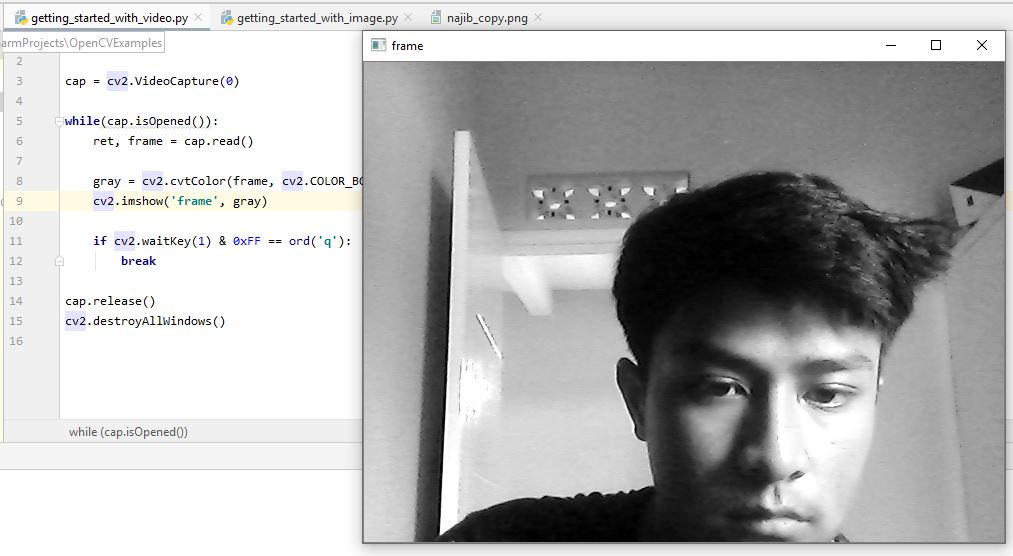
\includegraphics[scale=0.5]{figures/2,5.jpg}
\caption{Kontras warna video}
\label{contoh}
\end{figure}

Pada videocpture ini video sudah di rubah kontras warnanya menjadi abu abu, kita bisa rubah sesuai yang kita inginkan.

\newpage
\subsection{Mengetahui ukuran frame yang ditampilkan}
\lstinputlisting{src/cv6.py}
\begin{enumerate}
	\item lakukan Import library open cv yaitu cv2
	\item kemudian buat variable baru dengan nama cap kemudian panggil VideoCapture(0) yang artinya menjalankan kamera leptop.
	\item membuat while yaitu perulangan membuka frame
	\item kemudian didalam perulangan tersebut terdapat frame yang membaca atau merekam video.
	\item kita cukup print mengambil dari videocapture dan panggil CAP PROP FRAME WIDTH untuk mengetahui ukuran lebarnya dan CAP PROP FRAME HEIGHT untuk ukuran tingginya 
	\item buat variable dengan nama gray karna kita mau berubah kontras warnanya menjadi hitam putih, kemudian panggil cvtColor didalam frame dengan warna abu abu.
	\item kemudian buat frame dengan nama frame
	\item kemudian gunakan waitKey untuk membuat frame agar tidak langsung mati atau tertutup otomatis.
	\item release untuk menutup videocapture
	\item destroyAllWindows digunakan untuk menutup frame.
\end{enumerate}

\newpage
\begin{figure}[ht]
\centering
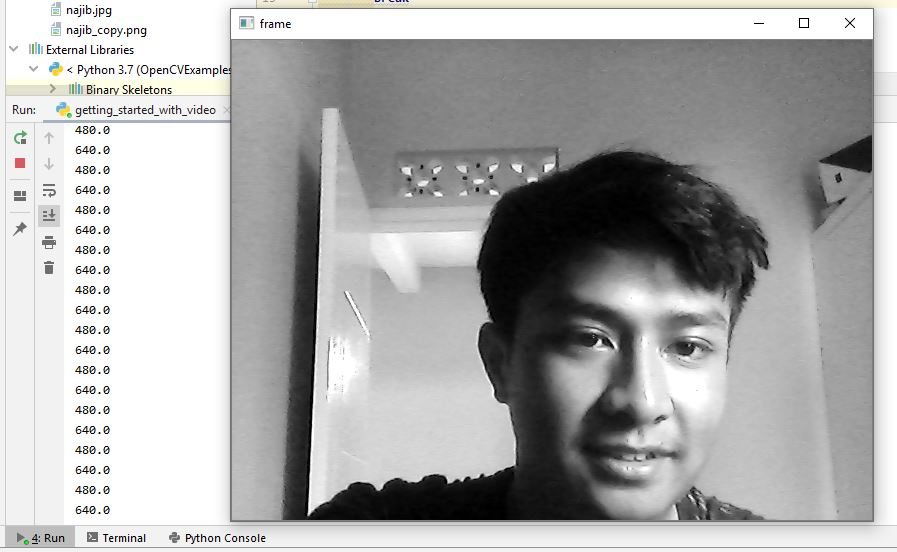
\includegraphics[scale=0.5]{figures/2,6.jpg}
\caption{Ukuran Frame video}
\label{contoh}
\end{figure}

Maka akan ditampilkan secara berulang karna berada pada while dan pada bagian videocapture juga jika tidak di lakukan perulangan maka sekali muncul akan langsung keluar secara otomatis.

\newpage
\subsection{Menyimpan video}
\lstinputlisting{src/cv7.py}
\begin{enumerate}
	\item lakukan Import library open cv yaitu cv2
	\item kemudian buat variable baru dengan nama cap kemudian panggil VideoCapture(0) yang artinya menjalankan kamera leptop.
	\item membuat variabel fourcc untuk merekam video yang dijalankan.
	\item membuat variable out untuk menyimpan video dengan nama najib.avi dan frame berukuran 640,480.
	\item melakukan print apakah true atau false kamera leptop terbuka.
	\item membuat while yaitu perulangan membuka frame
	\item kemudian didalam perulangan tersebut terdapat frame yang membaca atau merekam video.
	\item jika kamera true merekam maka akan melakukan perintah.
	\item kita cukup print mengambil dari videocapture dan panggil CAP PROP FRAME WIDTH untuk mengetahui ukuran lebarnya dan 
	\item kita cukup print mengambil dari videocapture dan panggil CAP PROP FRAME HEIGHT untuk ukuran tingginya 
	\item buat variable dengan nama gray karna kita mau berubah kontras warnanya menjadi hitam putih, kemudian panggil cvtColor didalam frame dengan warna abu abu.
	\item kemudian buat frame dengan nama frame
	\item kemudian gunakan waitKey untuk membuat frame agar tidak langsung mati atau tertutup otomatis.
	\item release untuk menutup videocapture
	\item destroyAllWindows digunakan untuk menutup frame.
\end{enumerate}

\begin{figure}[ht]
\centering
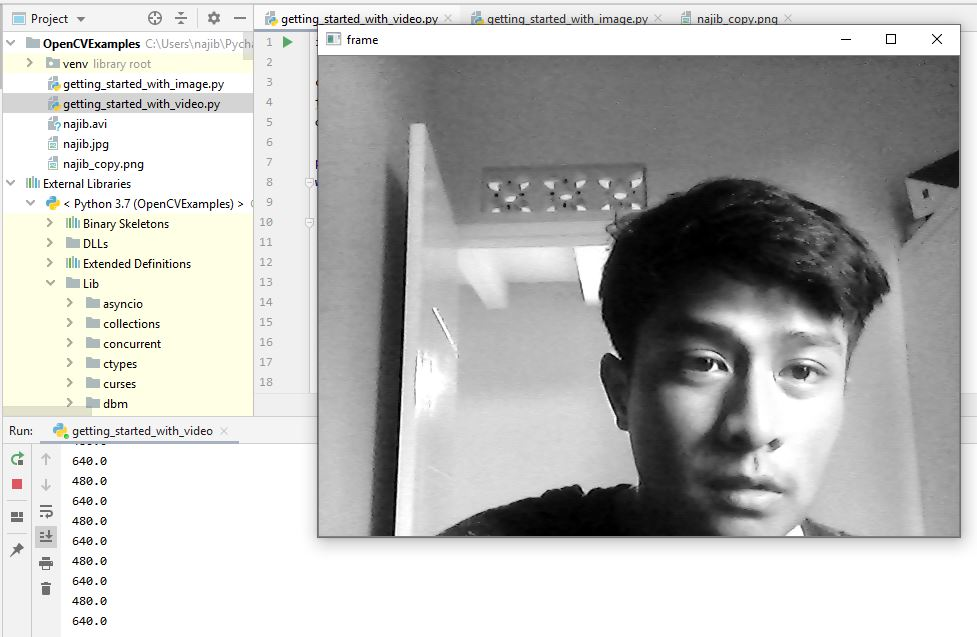
\includegraphics[scale=0.5]{figures/2,7.jpg}
\caption{Setelah dijalankan file tersimpan}
\label{contoh}
\end{figure}

\newpage
\begin{figure}[ht]
\centering
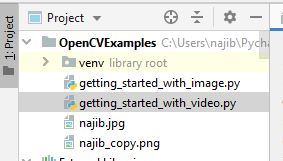
\includegraphics[scale=0.5]{figures/2,7,1.jpg}
\caption{File Sebelum dijalankan}
\label{contoh}
\end{figure}

\begin{figure}[ht]
\centering
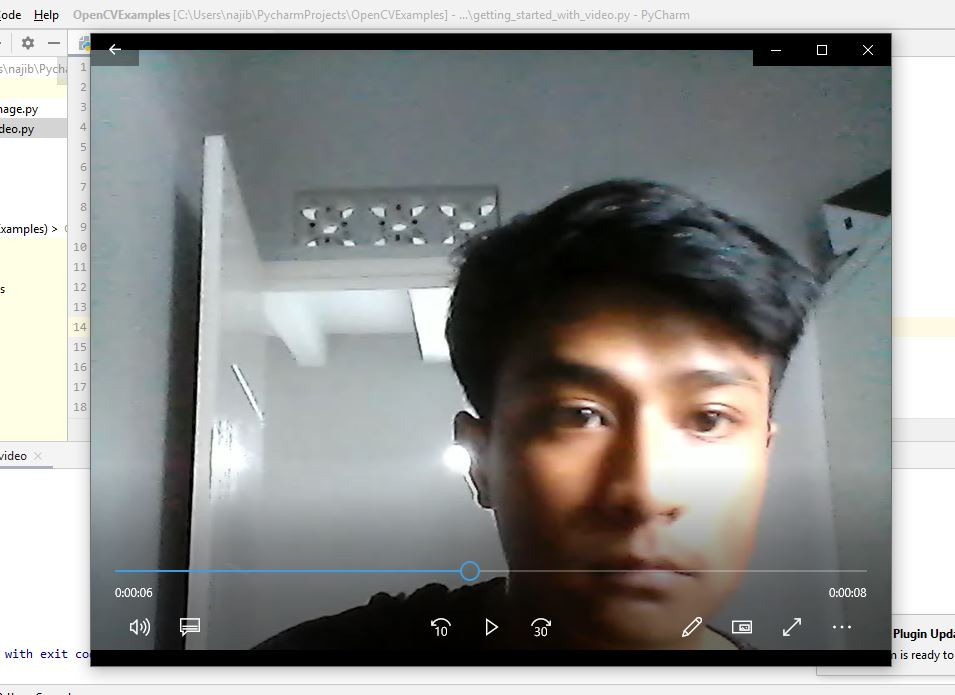
\includegraphics[scale=0.5]{figures/2,7,2.jpg}
\caption{Video yang sudah di simpan}
\label{contoh}
\end{figure}

Video tersimpan langsung ke folder yang dituju, video dapat disesuaikan formatnya sesuai yang kita mau.

\newpage
\section{Menggambar Geometric Pada Foto}
\subsection{Membuat garis}
\lstinputlisting{src/cv8.py}
\begin{enumerate}
	\item lakukan Import library open cv yaitu cv2
	\item kemudian panggil file foto menggunakan kode seperti di atas, membuat terlebihdahulu variabel img, kemudian cv2.imread nama file dan nomor untuk gradiasi warnanya, pada bagian ini menggunakan angka 0 yang artinya gambar berubah menjadi hitam putih.
	\item kemudian buat garis menggunakan cv2.line, 0,0 merupakan dimana titik awal garis tersebut dan 255,255 merupakan titik akhir dari garis tersebut, kemudian selanjutnya adahal warna dari garis tersebut, dan yang terakhir adalah ketebalan dari garis yang dibuat.
	\item kemudian buat frame untuk menampilkan gambar menggunakan imshow dengan nama frame image.
	\item kemudian gunakan waitKey untuk membuat frame agar tidak langsung mati atau tertutup otomatis.
	\item destroyAllWindows digunakan untuk menutup frame.
\end{enumerate}

\newpage
\begin{figure}[ht]
\centering
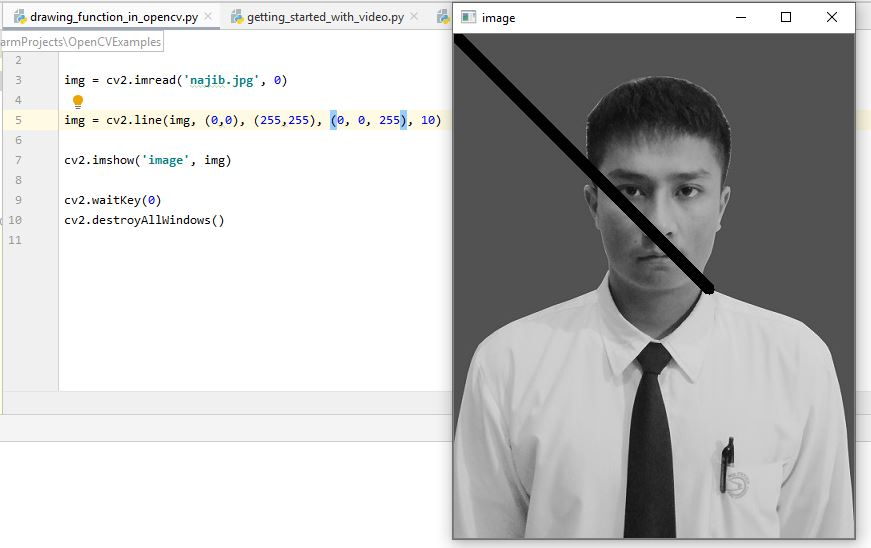
\includegraphics[scale=0.5]{figures/2,8.jpg}
\caption{MMembuat garis}
\label{contoh}
\end{figure}

garis bisa kita taruh dimana saja sesuai yang diinginkan kenapa garisnya menjulur dari pojok kiri atas ke tengah karna titik 0,0 berada di pojok kiri atas sedangkan titik 255,255 berada di tengah tengah gambar, gambar ini pun menjadi hitam putih karna di awal pada imread nya diberikan angka 0 yang membuat gambar berubah menjadi hitam putih.

\newpage
\subsection{Membuat warna warna pada garis}
\lstinputlisting{src/cv9.py}
\begin{enumerate}
	\item lakukan Import library open cv yaitu cv2
	\item kemudian panggil file foto menggunakan kode seperti di atas, membuat terlebihdahulu variabel img, kemudian cv2.imread nama file dan nomor untuk gradiasi warnanya, pada bagian ini menggunakan angka 1 yang artinya mengikuti foto aslinya.
	\item kemudian buat garis menggunakan cv2.line, 0,0 merupakan dimana titik awal garis tersebut dan 255,255 merupakan titik akhir dari garis tersebut, kemudian selanjutnya adalah warna dari garis tersebut, dan yang terakhir adalah ketebalan dari garis yang dibuat.
	\item kemudian buat frame untuk menampilkan gambar menggunakan imshow dengan nama frame image.
	\item kemudian gunakan waitKey untuk membuat frame agar tidak langsung mati atau tertutup otomatis.
	\item destroyAllWindows digunakan untuk menutup frame.
\end{enumerate}

\newpage
\begin{figure}[ht]
\centering
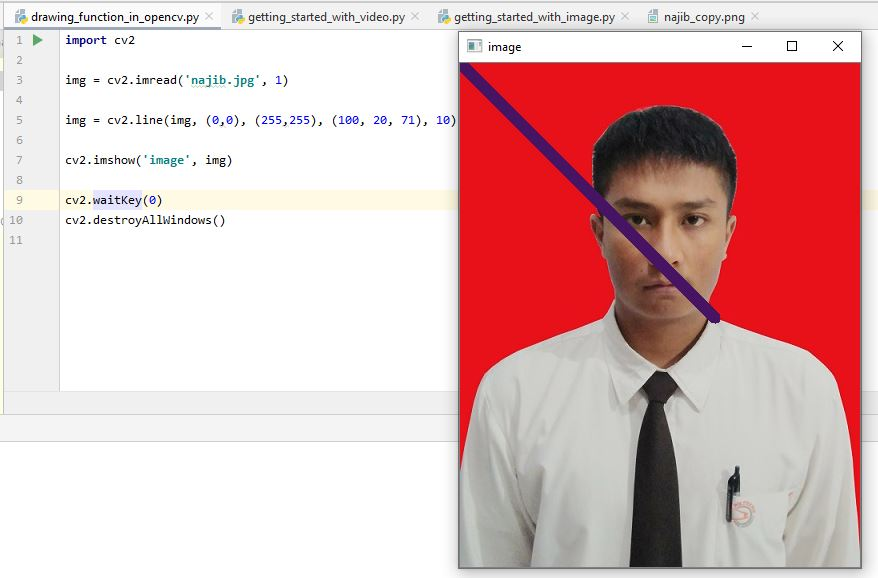
\includegraphics[scale=0.5]{figures/2,9.jpg}
\caption{Membuat garis}
\label{contoh}
\end{figure}

garis bisa kita taruh dimana saja sesuai yang diinginkan kenapa garisnya menjulur dari pojok kiri atas ke tengah karna titik 0,0 berada di pojok kiri atas sedangkan titik 255,255 berada di tengah tengah gambar, gambar menjadi seperti aslinya karna pada imreadnya 1.

\newpage
\begin{figure}[ht]
\centering
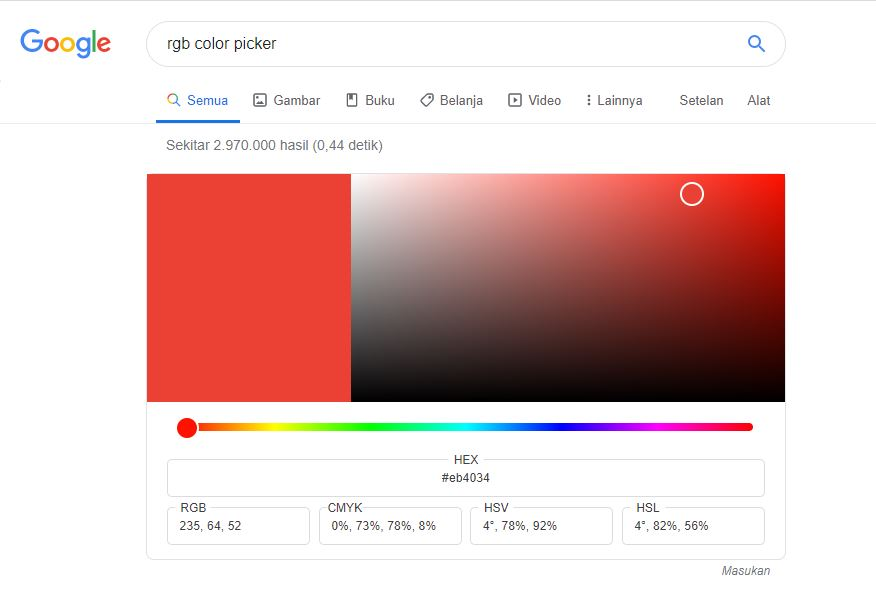
\includegraphics[scale=0.5]{figures/2,9,1.jpg}
\caption{Nomor Nomor warna}
\label{contoh}
\end{figure}

jika kita ingin warna yang sesuai dengan keinginan kita, kita bisa langsung search di google seperti pada gambar maka akan ada nomor nomornya untuk setiap warna.

\newpage
\subsection{Membuat garis panah}
\lstinputlisting{src/cv10.py}
\begin{enumerate}
	\item lakukan Import library open cv yaitu cv2
	\item kemudian panggil file foto menggunakan kode seperti di atas, membuat terlebihdahulu variabel img, kemudian cv2.imread nama file dan nomor untuk gradiasi warnanya, pada bagian ini menggunakan angka 1 yang artinya mengikuti foto aslinya.
	\item kemudian buat garis menggunakan cv2.line, 0,0 merupakan dimana titik awal garis tersebut dan 255,255 merupakan titik akhir dari garis tersebut, kemudian selanjutnya adalah warna dari garis tersebut, dan yang terakhir adalah ketebalan dari garis yang dibuat.
	\item kemudian buat garis panah menggunakan cv2.arrowedLine, 0,0 merupakan dimana titik awal garis tersebut dan 255,255 merupakan titik akhir dari garis tersebut, kemudian selanjutnya adalah warna dari garis tersebut, dan yang terakhir adalah ketebalan dari garis yang dibuat.
	\item kemudian buat frame untuk menampilkan gambar menggunakan imshow dengan nama frame image.
	\item kemudian gunakan waitKey untuk membuat frame agar tidak langsung mati atau tertutup otomatis.
	\item destroyAllWindows digunakan untuk menutup frame.
\end{enumerate}

\newpage
\begin{figure}[ht]
\centering
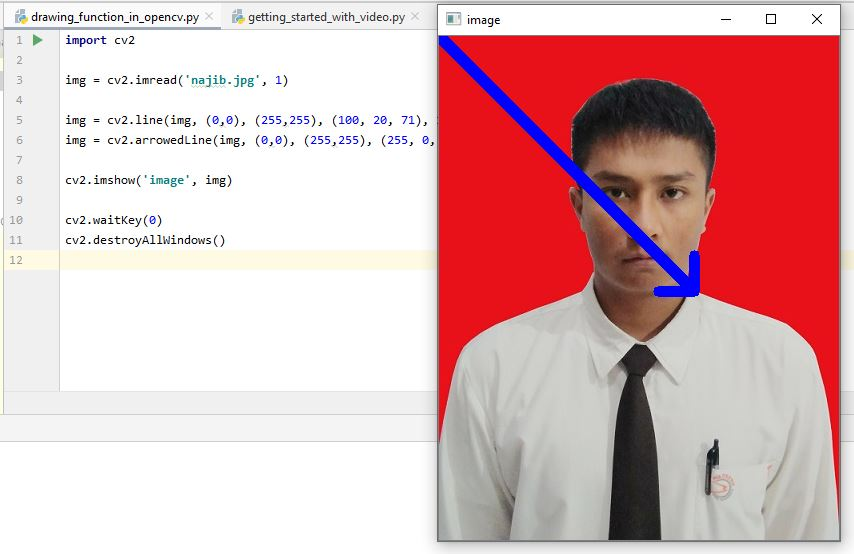
\includegraphics[scale=0.5]{figures/2,10.jpg}
\caption{Membuat garis panah}
\label{contoh}
\end{figure}

Garis panah yang dibuat menumpuk dengan garis yang awal jadi yang di lihat seperti garis yang sebelumnya hilang padahal garis tersebut tertumpuk.

\newpage
\subsection{Membuat garis kotak}
\lstinputlisting{src/cv11.py}
\begin{enumerate}
	\item lakukan Import library open cv yaitu cv2
	\item kemudian panggil file foto menggunakan kode seperti di atas, membuat terlebihdahulu variabel img, kemudian cv2.imread nama file dan nomor untuk gradiasi warnanya, pada bagian ini menggunakan angka 1 yang artinya mengikuti foto aslinya.
	\item kemudian buat garis menggunakan cv2.line, 0,0 merupakan dimana titik awal garis tersebut dan 255,255 merupakan titik akhir dari garis tersebut, kemudian selanjutnya adalah warna dari garis tersebut, dan yang terakhir adalah ketebalan dari garis yang dibuat.
	\item kemudian buat garis panah menggunakan cv2.arrowedLine, 0,0 merupakan dimana titik awal garis tersebut dan 255,255 merupakan titik akhir dari garis tersebut, kemudian selanjutnya adalah warna dari garis tersebut, dan yang terakhir adalah ketebalan dari garis yang dibuat.
	\item kemudian buat garis kotak menggunakan cv2.rectangle, 384,0 merupakan dimana titik awal garis tersebut dan 210,210 merupakan titik akhir dari garis tersebut, kemudian selanjutnya adalah warna dari garis tersebut, dan yang terakhir adalah ketebalan dari garis yang dibuat.
	\item kemudian buat frame untuk menampilkan gambar menggunakan imshow dengan nama frame image.
	\item kemudian gunakan waitKey untuk membuat frame agar tidak langsung mati atau tertutup otomatis.
	\item destroyAllWindows digunakan untuk menutup frame.
\end{enumerate}

\newpage
\begin{figure}[ht]
\centering
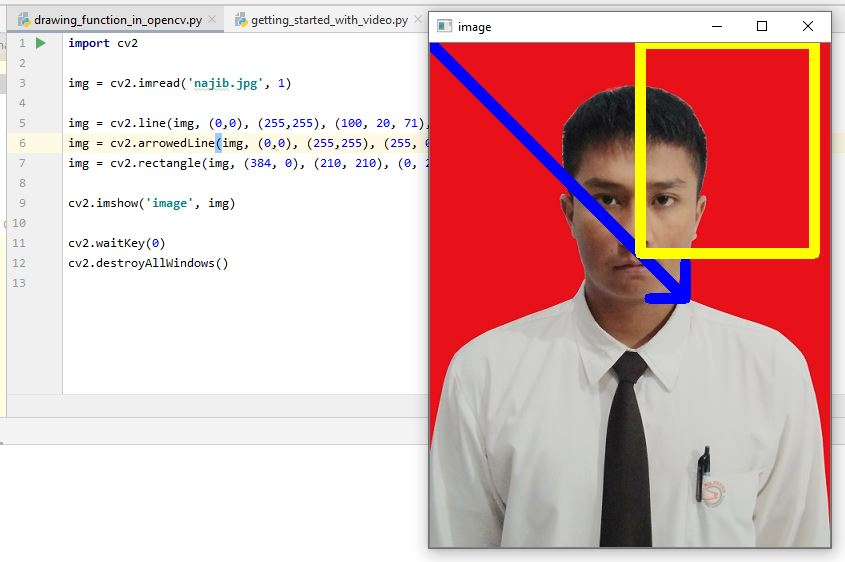
\includegraphics[scale=0.5]{figures/2,11.jpg}
\caption{Membuat garis kotak}
\label{contoh}
\end{figure}

Garis kotak ini bisa kita atur mau warna yang bagaimana, ukuran yang bagaimana, dan posisi yang bagaimana sesuai yang di inginkan dan sesuai kebutuhannya.

\newpage
\subsection{Membuat kotak}
\lstinputlisting{src/cv12.py}
\begin{enumerate}
	\item lakukan Import library open cv yaitu cv2
	\item kemudian panggil file foto menggunakan kode seperti di atas, membuat terlebihdahulu variabel img, kemudian cv2.imread nama file dan nomor untuk gradiasi warnanya, pada bagian ini menggunakan angka 1 yang artinya mengikuti foto aslinya.
	\item kemudian buat garis menggunakan cv2.line, 0,0 merupakan dimana titik awal garis tersebut dan 255,255 merupakan titik akhir dari garis tersebut, kemudian selanjutnya adalah warna dari garis tersebut, dan yang terakhir adalah ketebalan dari garis yang dibuat.
	\item kemudian buat garis panah menggunakan cv2.arrowedLine, 0,0 merupakan dimana titik awal garis tersebut dan 255,255 merupakan titik akhir dari garis tersebut, kemudian selanjutnya adalah warna dari garis tersebut, dan yang terakhir adalah ketebalan dari garis yang dibuat.
	\item kemudian buat garis kotak menggunakan cv2.rectangle, 384,0 merupakan dimana titik awal garis tersebut dan 210,210 merupakan titik akhir dari garis tersebut, kemudian selanjutnya adalah warna dari garis tersebut, dan yang terakhir adalah -1 yang membuat kotak terisi full karna jika plus yang membesar adalah bagian luarnya juka min yang membesar adalah bagian dalamnya jika minus maka akan full.
	\item kemudian buat frame untuk menampilkan gambar menggunakan imshow dengan nama frame image.
	\item kemudian gunakan waitKey untuk membuat frame agar tidak langsung mati atau tertutup otomatis.
	\item destroyAllWindows digunakan untuk menutup frame.
\end{enumerate}

\newpage
\begin{figure}[ht]
\centering
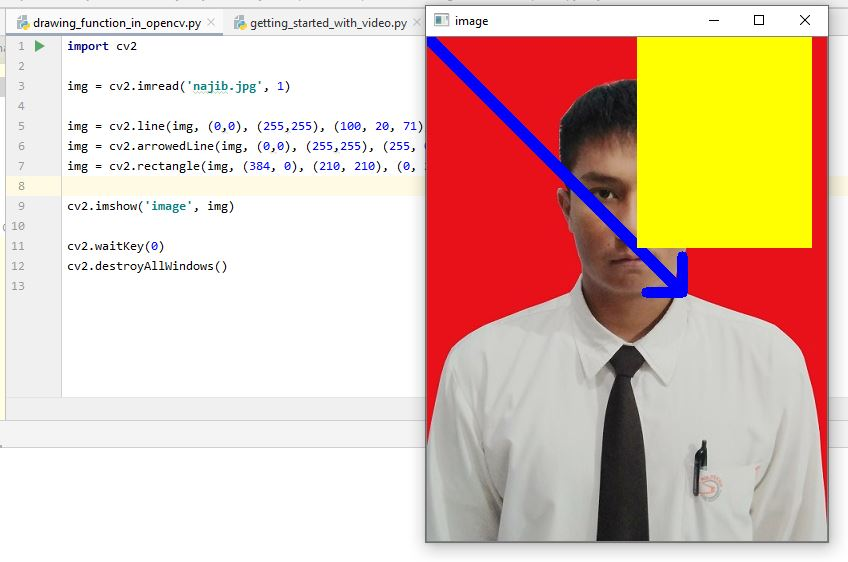
\includegraphics[scale=0.5]{figures/2,12.jpg}
\caption{Membuat kotak}
\label{contoh}
\end{figure}

Garis kotak ini bisa kita atur mau warna yang bagaimana, ukuran yang bagaimana, dan posisi yang bagaimana sesuai yang di inginkan dan sesuai kebutuhannya.

\newpage
\subsection{Membuat garis Lingkaran}
\lstinputlisting{src/cv13.py}
\begin{enumerate}
	\item lakukan Import library open cv yaitu cv2
	\item kemudian panggil file foto menggunakan kode seperti di atas, membuat terlebihdahulu variabel img, kemudian cv2.imread nama file dan nomor untuk gradiasi warnanya, pada bagian ini menggunakan angka 1 yang artinya mengikuti foto aslinya.
	\item kemudian buat garis menggunakan cv2.line, 0,0 merupakan dimana titik awal garis tersebut dan 255,255 merupakan titik akhir dari garis tersebut, kemudian selanjutnya adalah warna dari garis tersebut, dan yang terakhir adalah ketebalan dari garis yang dibuat.
	\item kemudian buat garis panah menggunakan cv2.arrowedLine, 0,0 merupakan dimana titik awal garis tersebut dan 255,255 merupakan titik akhir dari garis tersebut, kemudian selanjutnya adalah warna dari garis tersebut, dan yang terakhir adalah ketebalan dari garis yang dibuat.
	\item kemudian buat garis kotak menggunakan cv2.rectangle, 384,0 merupakan dimana titik awal garis tersebut dan 210,210 merupakan titik akhir dari garis tersebut, kemudian selanjutnya adalah warna dari garis tersebut, dan yang terakhir adalah ketebalan dari garis yang dibuat.
	\item kemudian buat garis kotak menggunakan cv2.circle, 320,63 merupakan dimana titik awal garis tersebut dan 63 merupakan titik tengah, kemudian selanjutnya adalah warna dari garis tersebut, dan yang terakhir adalah -1 yang membuat kotak terisi full karna jika plus yang membesar adalah bagian luarnya juka min yang membesar adalah bagian dalamnya jika minus maka akan full.
	\item kemudian buat frame untuk menampilkan gambar menggunakan imshow dengan nama frame image.
	\item kemudian gunakan waitKey untuk membuat frame agar tidak langsung mati atau tertutup otomatis.
	\item destroyAllWindows digunakan untuk menutup frame.
\end{enumerate}

\begin{figure}[ht]
\centering
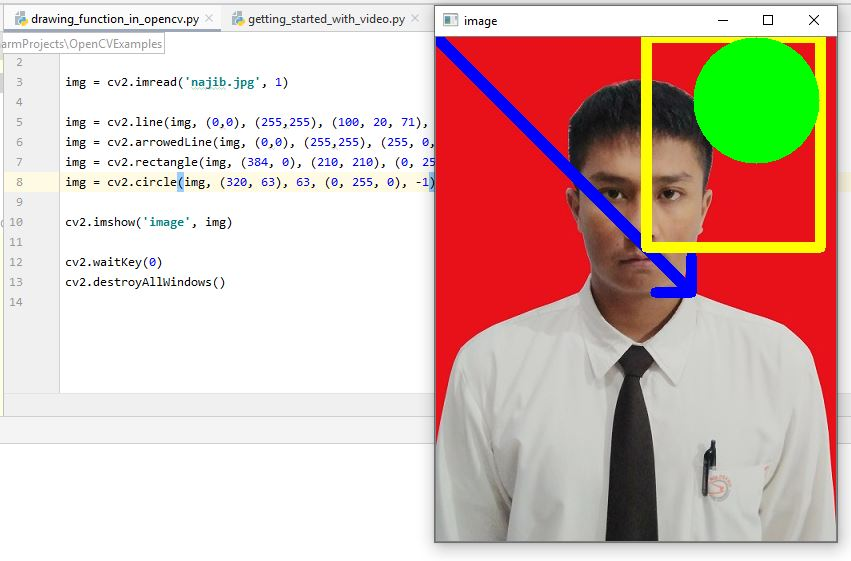
\includegraphics[scale=0.5]{figures/2,13.jpg}
\caption{Membuat garis lingkaran}
\label{contoh}
\end{figure}

Garis Lingkaran ini bisa kita atur mau warna yang bagaimana, ukuran yang bagaimana, dan posisi yang bagaimana sesuai yang di inginkan dan sesuai kebutuhannya.

\newpage
\subsection{Membuat Text}
\lstinputlisting{src/cv14.py}
\begin{enumerate}
	\item lakukan Import library open cv yaitu cv2
	\item kemudian panggil file foto menggunakan kode seperti di atas, membuat terlebihdahulu variabel img, kemudian cv2.imread nama file dan nomor untuk gradiasi warnanya, pada bagian ini menggunakan angka 1 yang artinya mengikuti foto aslinya.
	\item kemudian buat garis menggunakan cv2.line, 0,0 merupakan dimana titik awal garis tersebut dan 255,255 merupakan titik akhir dari garis tersebut, kemudian selanjutnya adalah warna dari garis tersebut, dan yang terakhir adalah ketebalan dari garis yang dibuat.
	\item kemudian buat garis panah menggunakan cv2.arrowedLine, 0,0 merupakan dimana titik awal garis tersebut dan 255,255 merupakan titik akhir dari garis tersebut, kemudian selanjutnya adalah warna dari garis tersebut, dan yang terakhir adalah ketebalan dari garis yang dibuat.
	\item kemudian buat garis kotak menggunakan cv2.rectangle, 384,0 merupakan dimana titik awal garis tersebut dan 210,210 merupakan titik akhir dari garis tersebut, kemudian selanjutnya adalah warna dari garis tersebut, dan yang terakhir adalah ketebalan dari garis yang dibuat.
	\item kemudian buat garis kotak menggunakan cv2.circle, 320,63 merupakan dimana titik awal garis tersebut dan 63 merupakan titik tengah, kemudian selanjutnya adalah warna dari garis tersebut, dan yang terakhir adalah -1 yang membuat kotak terisi full karna jika plus yang membesar adalah bagian luarnya juka min yang membesar adalah bagian dalamnya jika minus maka akan full.
	\item tentukan fontnya terlebih dahulu
	\item kemudian gunakan putText atur sesuai seperti pada gambar.
	\item kemudian buat frame untuk menampilkan gambar menggunakan imshow dengan nama frame image.
	\item kemudian gunakan waitKey untuk membuat frame agar tidak langsung mati atau tertutup otomatis.
	\item destroyAllWindows digunakan untuk menutup frame.
\end{enumerate}

\begin{figure}[ht]
\centering
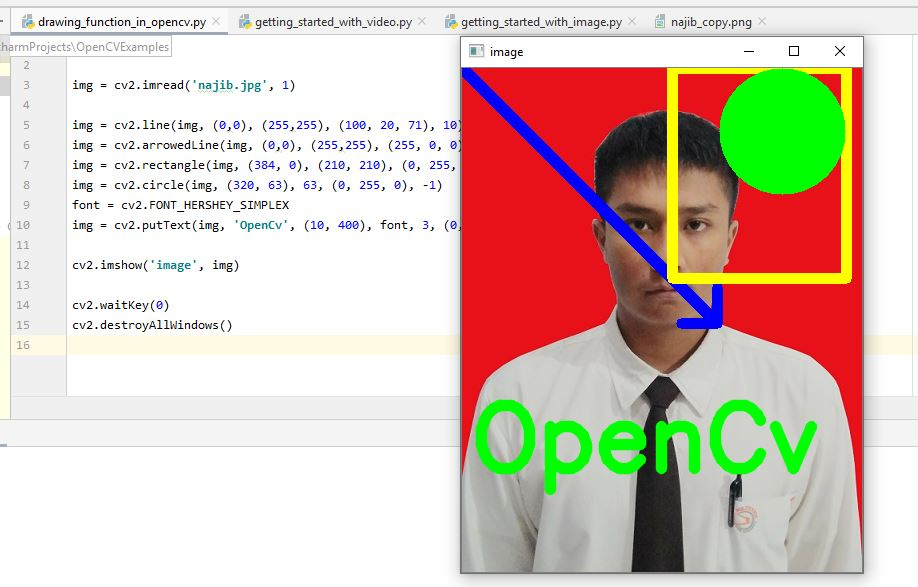
\includegraphics[scale=0.5]{figures/2,14.jpg}
\caption{Membuat Text}
\label{contoh}
\end{figure}

Text ini bisa kita buat sesuai kata kata yang di inginkan dan kata kata yang sesuai pada gambar, mau warna yang bagaimana, ukuran yang bagaimana, dan posisi yang bagaimana sesuai yang di inginkan dan sesuai kebutuhannya.

\newpage
\section{Frame Numpay}
\subsection{Membuat Frame menggunakan Numpay}
\lstinputlisting{src/cv15.py}
\begin{enumerate}
	\item lakukan import numpay as np
	\item lakukan Import library open cv yaitu cv2
	\item kemudian buat frame dari numpy yaitu zeros, kemudian ukuran fram dan warna dari fram, yang di buat adalah hitam.
	\item kemudian buat garis menggunakan cv2.line, 0,0 merupakan dimana titik awal garis tersebut dan 255,255 merupakan titik akhir dari garis tersebut, kemudian selanjutnya adalah warna dari garis tersebut, dan yang terakhir adalah ketebalan dari garis yang dibuat.
	\item kemudian buat garis panah menggunakan cv2.arrowedLine, 0,0 merupakan dimana titik awal garis tersebut dan 255,255 merupakan titik akhir dari garis tersebut, kemudian selanjutnya adalah warna dari garis tersebut, dan yang terakhir adalah ketebalan dari garis yang dibuat.
	\item kemudian buat garis kotak menggunakan cv2.rectangle, 384,0 merupakan dimana titik awal garis tersebut dan 210,210 merupakan titik akhir dari garis tersebut, kemudian selanjutnya adalah warna dari garis tersebut, dan yang terakhir adalah ketebalan dari garis yang dibuat.
	\item kemudian buat garis kotak menggunakan cv2.circle, 320,63 merupakan dimana titik awal garis tersebut dan 63 merupakan titik tengah, kemudian selanjutnya adalah warna dari garis tersebut, dan yang terakhir adalah -1 yang membuat kotak terisi full karna jika plus yang membesar adalah bagian luarnya juka min yang membesar adalah bagian dalamnya jika minus maka akan full.
	\item tentukan fontnya terlebih dahulu
	\item kemudian gunakan putText atur sesuai seperti pada gambar.
	\item kemudian buat frame untuk menampilkan gambar menggunakan imshow dengan nama frame image.
	\item kemudian gunakan waitKey untuk membuat frame agar tidak langsung mati atau tertutup otomatis.
	\item destroyAllWindows digunakan untuk menutup frame.
\end{enumerate}

\begin{figure}[ht]
\centering
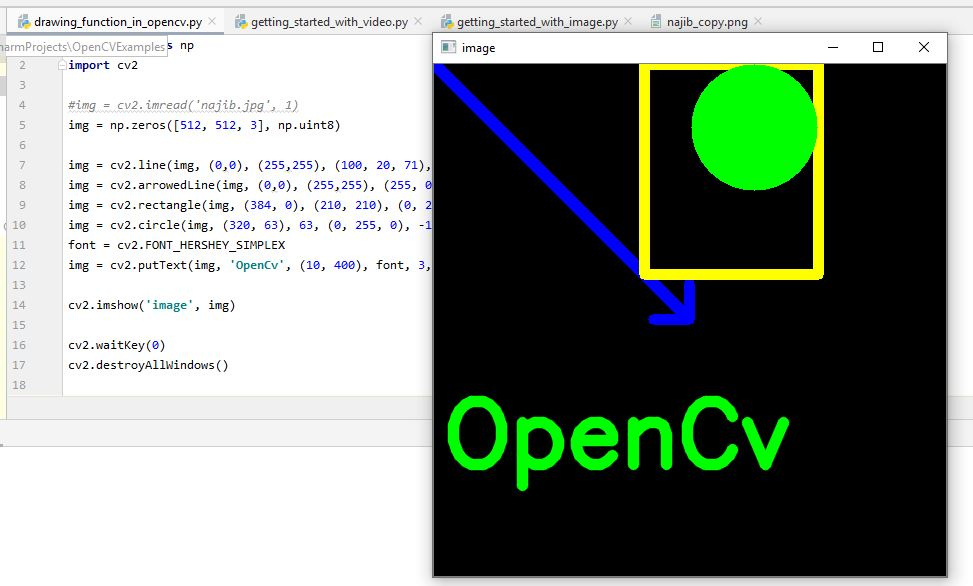
\includegraphics[scale=0.5]{figures/2,15.jpg}
\caption{Membuat Frame Numpy}
\label{contoh}
\end{figure}

Frame ini dibuat menggunakan matriks yang ada pada library numpay, kita tidak perlu lagi menghitung berapa matriksnya kita cukup gunakan zeros dan ukuran yang di butuhkan.

\newpage
\subsection{Berubah Ukuran Frame}
\lstinputlisting{src/cv16.py}
\begin{enumerate}
	\item import cv2
	\item membuat variable cap untuk menghubungkan kamera leptop
	\item print ukuran frame lebar dan tinggi menggunakan CAP PROP FRAME WIDTH dan CAP PROP FRAME HEIGHT
	\item membuat ukuran frame baru, jika ukurannya tidak sesuai maka akan otomatis mengikuti ukutan sebelumnya.
	\item print untuk menampilkan ukuran frame saat ini
	\item membuat while yaitu perulangan membuka frame
	\item kemudian didalam perulangan tersebut terdapat frame yang membaca atau merekam video.
	\item jika kamera true merekam maka akan melakukan perintah. 
	\item buat variable dengan nama gray karna kita mau berubah kontras warnanya menjadi hitam putih, kemudian panggil cvtColor didalam frame dengan warna abu abu.
	\item kemudian buat frame dengan nama frame
	\item kemudian gunakan waitKey untuk membuat frame agar tidak langsung mati atau tertutup otomatis.
	\item release untuk menutup videocapture
	\item destroyAllWindows digunakan untuk menutup frame.
\end{enumerate}

\begin{figure}[ht]
\centering
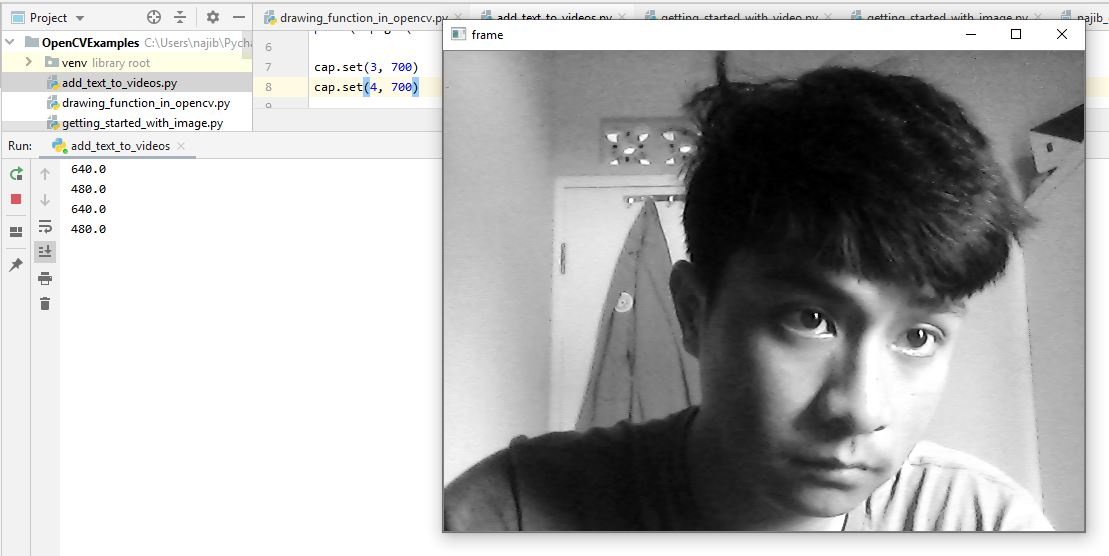
\includegraphics[scale=0.4]{figures/2,16.jpg}
\caption{Merubah ukuran frame}
\label{contoh}
\end{figure}



\newpage
\subsection{Menampilkan Text pada Frame video}
\lstinputlisting{src/cv17.py}
\begin{enumerate}
	\item import cv2
	\item membuat variable cap untuk menghubungkan kamera leptop
	\item print ukuran frame lebar dan tinggi menggunakan CAP PROP FRAME WIDTH dan CAP PROP FRAME HEIGHT
	\item membuat ukuran frame baru, jika ukurannya tidak sesuai maka akan otomatis mengikuti ukutan sebelumnya.
	\item print untuk menampilkan ukuran frame saat ini
	\item membuat while yaitu perulangan membuka frame
	\item kemudian didalam perulangan tersebut terdapat frame yang membaca atau merekam video.
	\item jika kamera true merekam maka akan melakukan perintah. 
	\item membuat font untuk tulisan pada gambar
	\item menampilkan tulisan ukuran frame
	\item menampilkan tulisan pada frame
	\item kemudian buat frame dengan nama frame
	\item kemudian gunakan waitKey untuk membuat frame agar tidak langsung mati atau tertutup otomatis.
	\item release untuk menutup videocapture
	\item destroyAllWindows digunakan untuk menutup frame.
\end{enumerate}

\begin{figure}[ht]
\centering
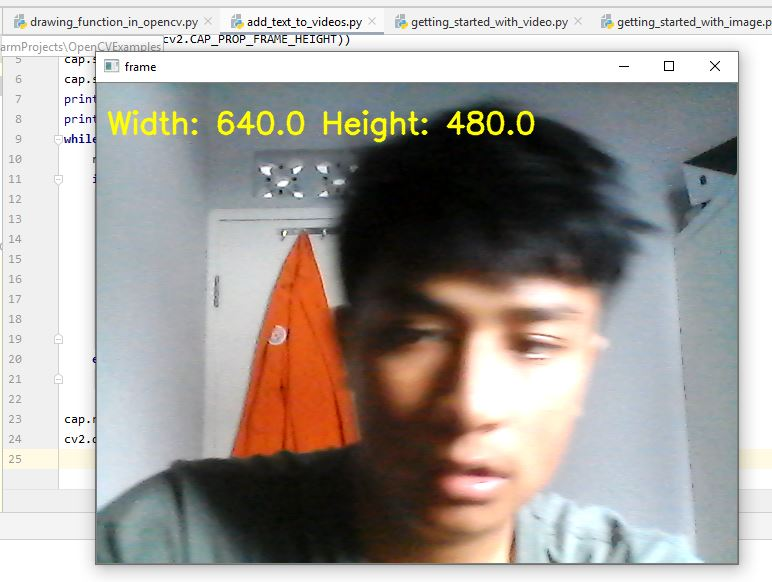
\includegraphics[scale=0.5]{figures/2,17.jpg}
\caption{Menampilkan Text pada Frame video}
\label{contoh}
\end{figure}



\newpage
\subsection{Menampilakn waktu pada frame}
\lstinputlisting{src/cv18.py}
\begin{enumerate}
	\item import cv2
	\item import date time
	\item membuat variable cap untuk menghubungkan kamera leptop
	\item print ukuran frame lebar dan tinggi menggunakan CAP PROP FRAME WIDTH dan CAP PROP FRAME HEIGHT
	\item membuat while yaitu perulangan membuka frame
	\item kemudian didalam perulangan tersebut terdapat frame yang membaca atau merekam video.
	\item jika kamera true merekam maka akan melakukan perintah. 
	\item membuat font untuk tulisan pada gambar
	\item menampilkan tulisan ukuran frame
	\item menampilkan tulisan tanggal dan waktu pada frame
	\item kemudian buat frame dengan nama frame
	\item kemudian gunakan waitKey untuk membuat frame agar tidak langsung mati atau tertutup otomatis.
	\item release untuk menutup videocapture
	\item destroyAllWindows digunakan untuk menutup frame.
\end{enumerate}

\begin{figure}[ht]
\centering
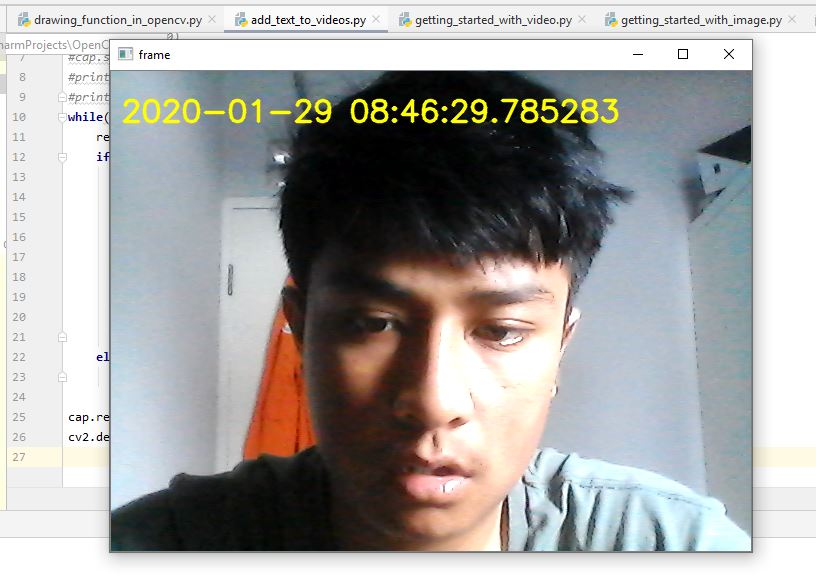
\includegraphics[scale=0.5]{figures/2,18.jpg}
\caption{Menampilakn waktu pada frame}
\label{contoh}
\end{figure}



\newpage
\subsection{Menampilkan Event}
\lstinputlisting{src/cv19.py}
\begin{enumerate}
	\item Import numpy
	\item import cv2
	\item menampilkan even event yang dapat digunakan untuk mouse klik
	\item menampilkannya dengan print
\end{enumerate}

\begin{figure}[ht]
\centering
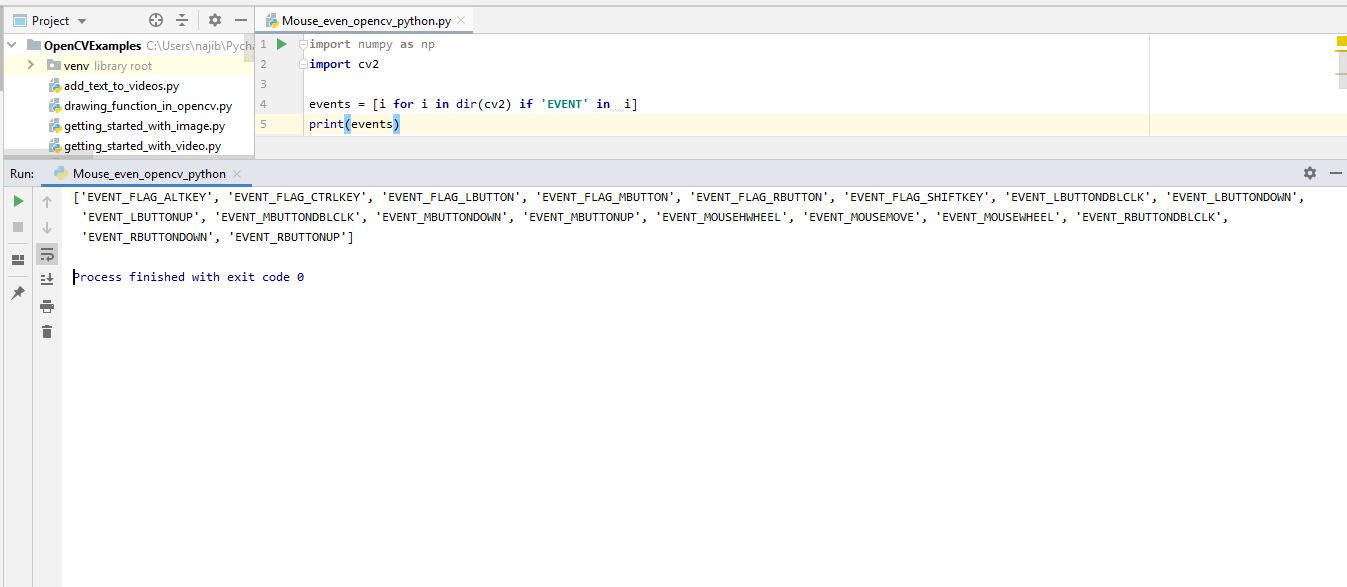
\includegraphics[scale=0.5]{figures/2,19.jpg}
\caption{Menampilkan Event}
\label{contoh}
\end{figure}



\newpage
\subsection{Event Mouse klik kiri}
\lstinputlisting{src/cv20.py}
\begin{enumerate}
	\item Import numpy
	\item import cv2
	\item buat def dengan nama click event
	\item jika mouse mengklik kiri maka akan melakukan sesuatu
	\item pada frame akan menampilkan posisi pada frame yang di klik
	\item membuat frame dengan ukuran 512 512 dengan warna hitam
	\item menampilkan frame dengan nama image
	\item memanggil fungsi klik pada mouse
	\item kemudian gunakan waitKey untuk membuat frame agar tidak langsung mati atau tertutup otomatis.
	\item destroyAllWindows digunakan untuk menutup frame.
\end{enumerate}

\newpage
\begin{figure}[ht]
\centering
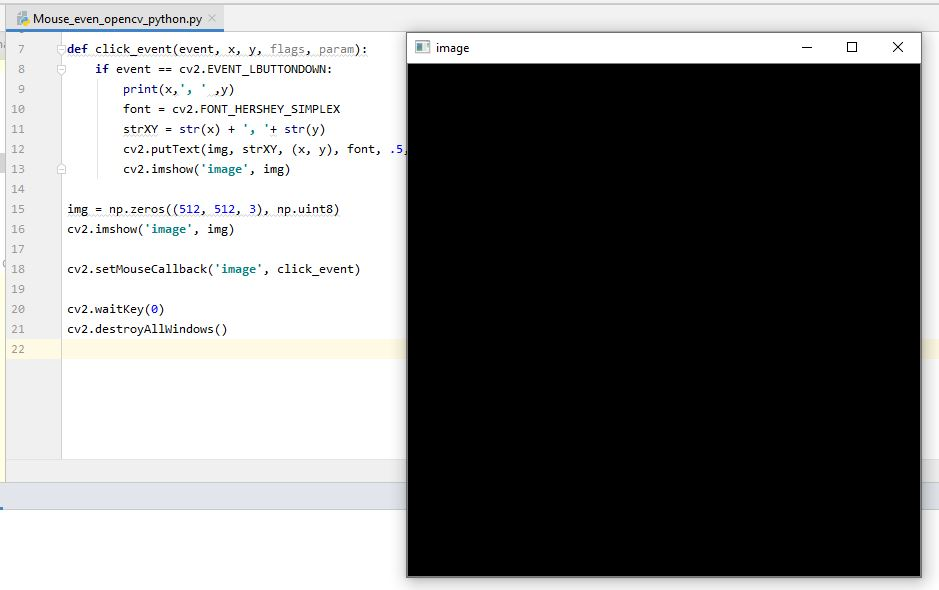
\includegraphics[scale=0.4]{figures/2,20.jpg}
\caption{Event Mouse klik kiri}
\label{contoh}
\end{figure}

\begin{figure}[ht]
\centering
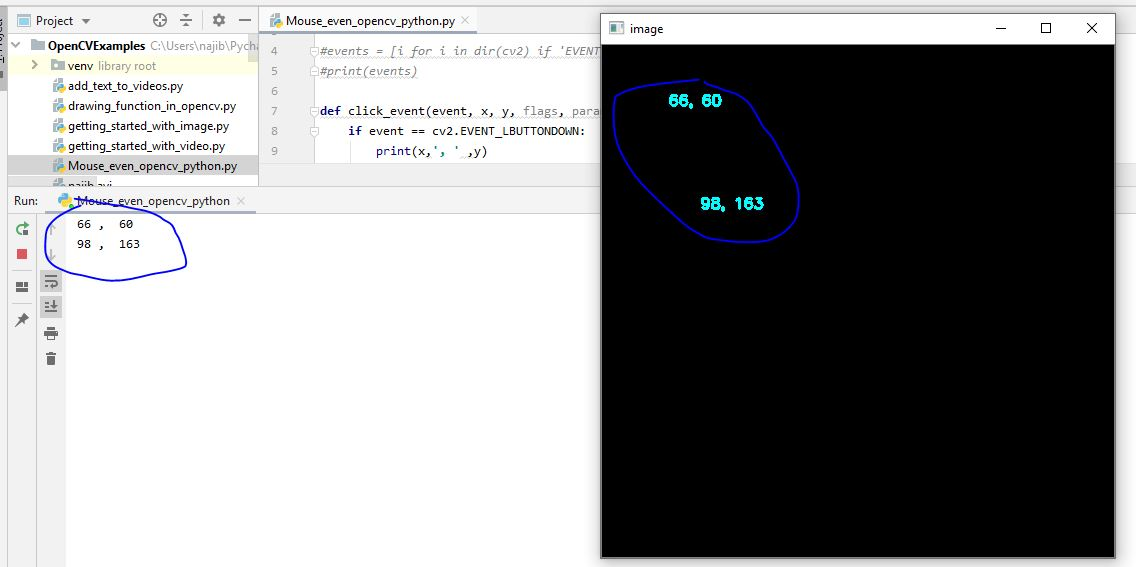
\includegraphics[scale=0.4]{figures/2,20,1.jpg}
\caption{Event Mouse klik kiri}
\label{contoh}
\end{figure}

\newpage
\begin{figure}[ht]
\centering
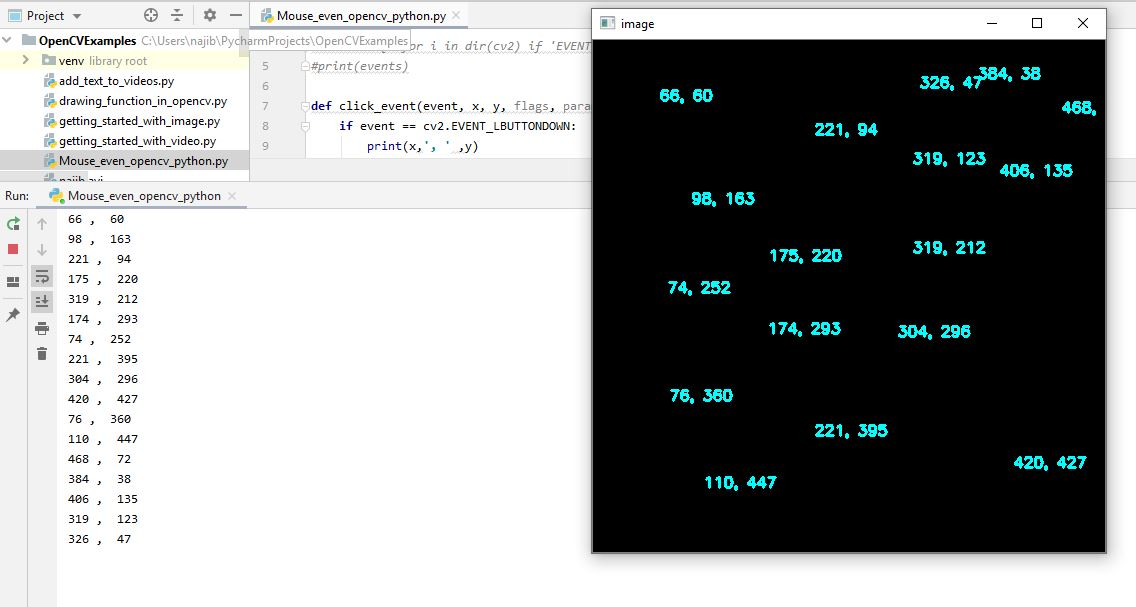
\includegraphics[scale=0.4]{figures/2,20,2.jpg}
\caption{Event Mouse klik kiri}
\label{contoh}
\end{figure}



\newpage
\subsection{Event Mouse klik kiri dan kanan}
\lstinputlisting{src/cv21.py}
\begin{enumerate}
	\item Import numpy
	\item import cv2
	\item buat def dengan nama click event
	\item jika mouse mengklik kiri maka akan melakukan sesuatu
	\item pada frame akan menampilkan posisi pada frame yang di klik
	\item dan jika mouse mengklik kanan
	\item maka frame akan menampilkan nomor warna yanga ada pada frame yang di klik tersebut, terdapat 3 nomor karna menggunakan konsep bgr yaitu blue green dan red.
	\item membuat frame dengan ukuran 512 512 dengan warna hitam
	\item menampilkan frame dengan nama image
	\item memanggil fungsi klik pada mouse
	\item kemudian gunakan waitKey untuk membuat frame agar tidak langsung mati atau tertutup otomatis.
	\item destroyAllWindows digunakan untuk menutup frame.
\end{enumerate}

\begin{figure}[ht]
\centering
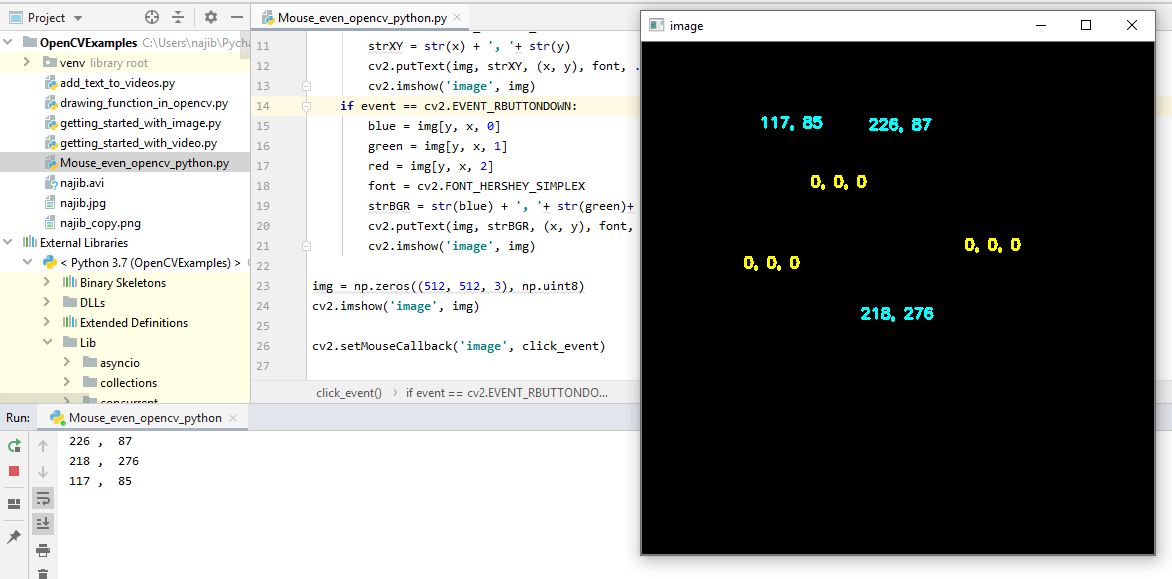
\includegraphics[scale=0.4]{figures/2,21.jpg}
\caption{Event Mouse klik kiri dan kanan}
\label{contoh}
\end{figure}



\newpage
\subsection{Event Mouse klik kiri dan kanan pada gambar yang dipangggil}
\lstinputlisting{src/cv22.py}
\begin{enumerate}
	\item Import numpy
	\item import cv2
	\item buat def dengan nama click event
	\item jika mouse mengklik kiri maka akan melakukan sesuatu
	\item pada frame akan menampilkan posisi pada frame yang di klik
	\item dan jika mouse mengklik kanan
	\item maka frame akan menampilkan nomor warna yanga ada pada frame yang di klik tersebut, terdapat 3 nomor karna menggunakan konsep bgr yaitu blue green dan red.
	\item memanggil gambar untuk di taruh pada frame yang telah di buat
	\item menampilkan frame dengan nama image
	\item memanggil fungsi klik pada mouse
	\item kemudian gunakan waitKey untuk membuat frame agar tidak langsung mati atau tertutup otomatis.
	\item destroyAllWindows digunakan untuk menutup frame.
\end{enumerate}

\begin{figure}[ht]
\centering
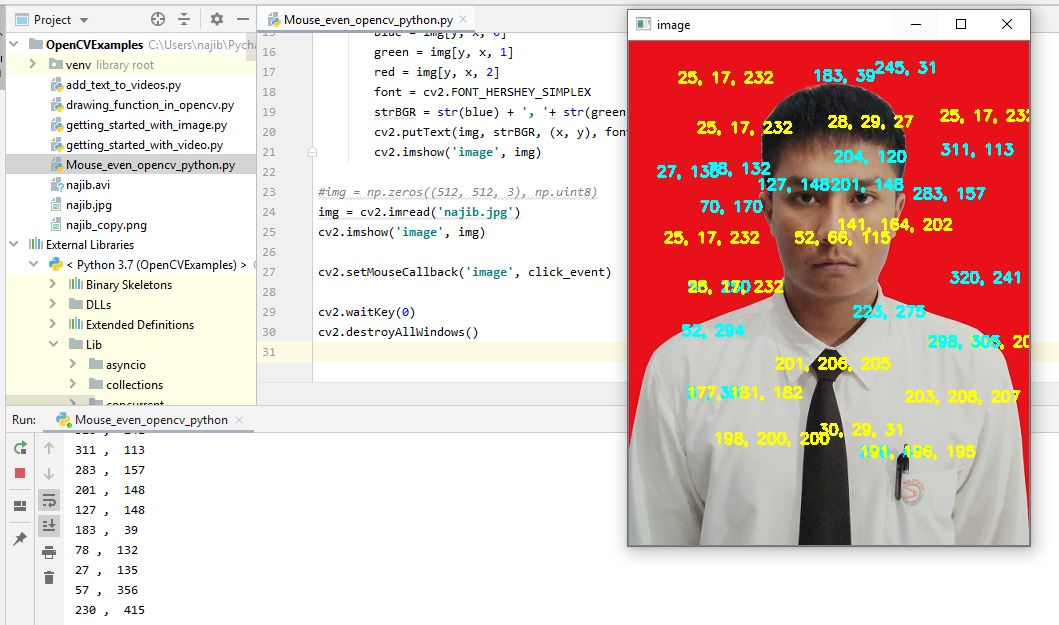
\includegraphics[scale=0.5]{figures/2,22.jpg}
\caption{Event Mouse klik kiri dan kanan pada gambar yang dipangggil}
\label{contoh}
\end{figure}



\newpage
\subsection{Event Mouse klik kiri membuat titik dan garis}
\lstinputlisting{src/cv23.py}
\begin{enumerate}
	\item Import numpy
	\item import cv2
	\item buat def dengan nama click event
	\item jika mouse mengklik kiri maka akan melakukan sesuatu
	\item pada frame akan membuat sebuah titik berwarna merah sesuai lokasi mengklik frame
	\item jika titik tersebut lebih dari sama dengan 2 maka setiap titik yang terakhir akan terhubung satu sama lain.
	\item menampilkan frame dengan nama image
	\item gambar pada frame berwarna hitam
	\item menampilkan frame kembali
	\item point menghilang setelah berubah menjadi garis atau line
	\item memanggil fungsi klik pada mouse
	\item kemudian gunakan waitKey untuk membuat frame agar tidak langsung mati atau tertutup otomatis.
	\item destroyAllWindows digunakan untuk menutup frame.
\end{enumerate}

\newpage
\begin{figure}[ht]
\centering
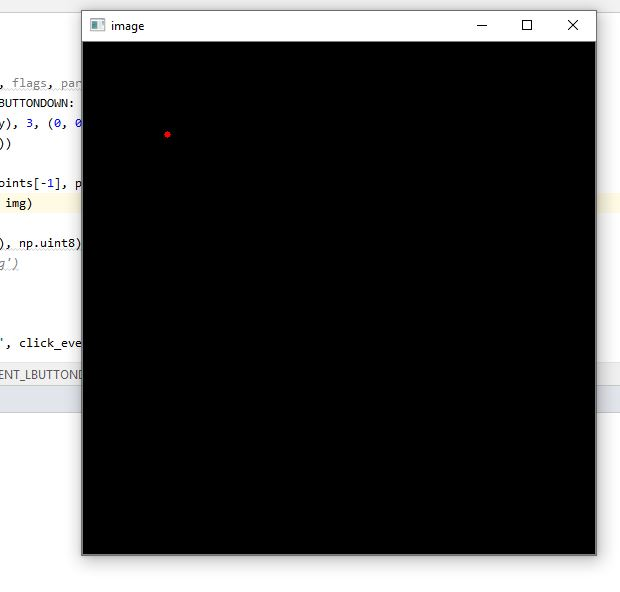
\includegraphics[scale=0.5]{figures/2,23.jpg}
\caption{Event Mouse klik kiri membuat titik dan garis}
\label{contoh}
\end{figure}

\begin{figure}[ht]
\centering
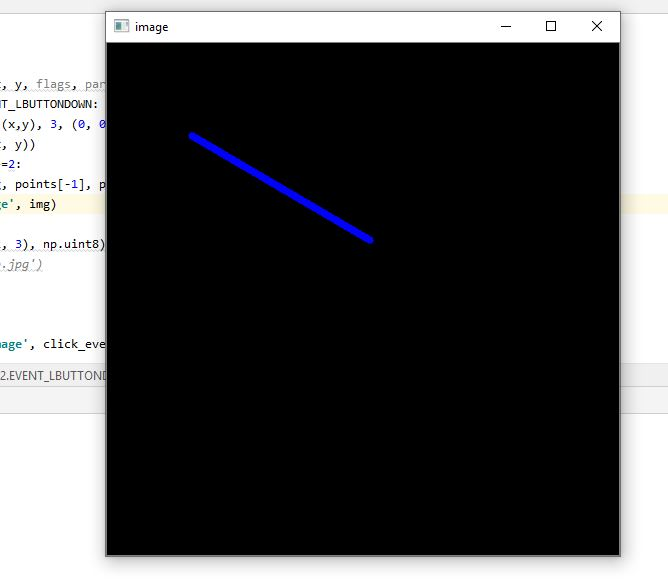
\includegraphics[scale=0.4]{figures/2,23,1.jpg}
\caption{Event Mouse klik kiri membuat titik dan garis}
\label{contoh}
\end{figure}

\newpage
\begin{figure}[ht]
\centering
\includegraphics[scale=0.5]{figures/2,23,2.jpg}
\caption{Event Mouse klik kiri membuat titik dan garis}
\label{contoh}
\end{figure}



\newpage
\subsection{Membuat frame warna sesuai klik}
\lstinputlisting{src/cv24.py}
\begin{enumerate}
	\item Import numpy
	\item import cv2
	\item buat def dengan nama click event
	\item jika mouse mengklik kiri maka akan melakukan sesuatu
	\item warna biru di deklarasikan dengan 0
	\item warna hijau di deklarasikan dengan 1
	\item warna merah di deklarasikan dengan 2
	\item membuat lingkaran kecil berwarna merah
	\item membuat warna sesuai lokasi frame yang di klik harus sesuai dengan warna yang di klik
	\item memanggil gambar
	\item menampilkan frame kembali
	\item point menghilang setelah berubah menjadi garis atau line
	\item memanggil fungsi klik pada mouse
	\item kemudian gunakan waitKey untuk membuat frame agar tidak langsung mati atau tertutup otomatis.
	\item destroyAllWindows digunakan untuk menutup frame.

\end{enumerate}

\begin{figure}[ht]
\centering
\includegraphics[scale=0.4]{figures/2,24.jpg}
\caption{Membuat frame warna sesuai klik}
\label{contoh}
\end{figure}

\newpage
\begin{figure}[ht]
\centering
\includegraphics[scale=0.4]{figures/2,24,1.jpg}
\caption{Membuat frame warna sesuai klik}
\label{contoh}
\end{figure}

\begin{figure}[ht]
\centering
\includegraphics[scale=0.4]{figures/2,24,2.jpg}
\caption{Membuat frame warna sesuai klik}
\label{contoh}
\end{figure}



\newpage
\subsection{Membuat frame warna sesuai klik 2}
\lstinputlisting{src/cv25.py}
\begin{enumerate}
	\item Import numpy
	\item import cv2
	\item buat def dengan nama click event
	\item jika mouse mengklik kiri maka akan melakukan sesuatu
	\item warna biru di deklarasikan dengan 0
	\item warna hijau di deklarasikan dengan 1
	\item warna merah di deklarasikan dengan 2
	\item membuat lingkaran kecil berwarna merah
	\item membuat warna sesuai lokasi frame yang di klik harus sesuai dengan warna yang di klik
	\item menggunakan gambar hitam
	\item menampilkan frame kembali
	\item point menghilang setelah berubah menjadi garis atau line
	\item memanggil fungsi klik pada mouse
	\item kemudian gunakan waitKey untuk membuat frame agar tidak langsung mati atau tertutup otomatis.
	\item destroyAllWindows digunakan untuk menutup frame.
\end{enumerate}

\begin{figure}[ht]
\centering
\includegraphics[scale=0.4]{figures/2,25.jpg}
\caption{Membuat frame warna sesuai klik 2}
\label{contoh}
\end{figure}



\newpage
\subsection{Berubah Ukuran Frame}
\lstinputlisting{src/cv26.py}
\begin{enumerate}
	\item
\end{enumerate}

\newpage
\begin{figure}[ht]
\centering
\includegraphics[scale=0.5]{figures/2,26.jpg}
\caption{Membuat Frame Numpy}
\label{contoh}
\end{figure}



\newpage
\subsection{Berubah Ukuran Frame}
\lstinputlisting{src/cv27.py}
\begin{enumerate}
	\item
\end{enumerate}

\newpage
\begin{figure}[ht]
\centering
\includegraphics[scale=0.5]{figures/2,27.jpg}
\caption{Membuat Frame Numpy}
\label{contoh}
\end{figure}



\newpage
\subsection{Berubah Ukuran Frame}
\lstinputlisting{src/cv28.py}
\begin{enumerate}
	\item
\end{enumerate}

\begin{figure}[ht]
\centering
\includegraphics[scale=0.5]{figures/2,28.jpg}
\caption{Membuat Frame Numpy}
\label{contoh}
\end{figure}



\newpage
\subsection{Berubah Ukuran Frame}
\lstinputlisting{src/cv29.py}
\begin{enumerate}
	\item
\end{enumerate}

\begin{figure}[ht]
\centering
\includegraphics[scale=0.5]{figures/2,29.jpg}
\caption{Membuat Frame Numpy}
\label{contoh}
\end{figure}



\newpage
\subsection{Berubah Ukuran Frame}
\lstinputlisting{src/cv30.py}
\begin{enumerate}
	\item
\end{enumerate}

\begin{figure}[ht]
\centering
\includegraphics[scale=0.5]{figures/2,30.jpg}
\caption{Membuat Frame Numpy}
\label{contoh}
\end{figure}

\begin{figure}[ht]
\centering
\includegraphics[scale=0.5]{figures/2,30,1.jpg}
\caption{Membuat Frame Numpy}
\label{contoh}
\end{figure}



\newpage
\subsection{Berubah Ukuran Frame}
\lstinputlisting{src/cv31.py}
\begin{enumerate}
	\item
\end{enumerate}

\begin{figure}[ht]
\centering
\includegraphics[scale=0.5]{figures/2,31.jpg}
\caption{Membuat Frame Numpy}
\label{contoh}
\end{figure}

\begin{figure}[ht]
\centering
\includegraphics[scale=0.5]{figures/2,31,1.jpg}
\caption{Membuat Frame Numpy}
\label{contoh}
\end{figure}



\newpage
\subsection{Berubah Ukuran Frame}
\lstinputlisting{src/cv32.py}
\begin{enumerate}
	\item
\end{enumerate}

\begin{figure}[ht]
\centering
\includegraphics[scale=0.5]{figures/2,32.jpg}
\caption{Membuat Frame Numpy}
\label{contoh}
\end{figure}

\begin{figure}[ht]
\centering
\includegraphics[scale=0.5]{figures/2,32,1.jpg}
\caption{Membuat Frame Numpy}
\label{contoh}
\end{figure}



\newpage
\subsection{Berubah Ukuran Frame}
\lstinputlisting{src/cv33.py}
\begin{enumerate}
	\item
\end{enumerate}

\begin{figure}[ht]
\centering
\includegraphics[scale=0.5]{figures/2,33.jpg}
\caption{Membuat Frame Numpy}
\label{contoh}
\end{figure}

\begin{figure}[ht]
\centering
\includegraphics[scale=0.5]{figures/2,33,1.jpg}
\caption{Membuat Frame Numpy}
\label{contoh}
\end{figure}

\begin{figure}[ht]
\centering
\includegraphics[scale=0.5]{figures/2,33,2.jpg}
\caption{Membuat Frame Numpy}
\label{contoh}
\end{figure}



\newpage
\subsection{Berubah Ukuran Frame}
\lstinputlisting{src/cv34.py}
\begin{enumerate}
	\item
\end{enumerate}

\begin{figure}[ht]
\centering
\includegraphics[scale=0.5]{figures/2,34.jpg}
\caption{Membuat Frame Numpy}
\label{contoh}
\end{figure}



\newpage
\subsection{Berubah Ukuran Frame}
\lstinputlisting{src/cv35.py}
\begin{enumerate}
	\item
\end{enumerate}

\begin{figure}[ht]
\centering
\includegraphics[scale=0.5]{figures/2,35.jpg}
\caption{Membuat Frame Numpy}
\label{contoh}
\end{figure}



\newpage
\subsection{Berubah Ukuran Frame}
\lstinputlisting{src/cv36.py}
\begin{enumerate}
	\item
\end{enumerate}

\begin{figure}[ht]
\centering
\includegraphics[scale=0.5]{figures/2,36.jpg}
\caption{Membuat Frame Numpy}
\label{contoh}
\end{figure}

\begin{figure}[ht]
\centering
\includegraphics[scale=0.5]{figures/2,36,1.jpg}
\caption{Membuat Frame Numpy}
\label{contoh}
\end{figure}

\begin{figure}[ht]
\centering
\includegraphics[scale=0.5]{figures/2,36,2.jpg}
\caption{Membuat Frame Numpy}
\label{contoh}
\end{figure}

\begin{figure}[ht]
\centering
\includegraphics[scale=0.5]{figures/2,36,3.jpg}
\caption{Membuat Frame Numpy}
\label{contoh}
\end{figure}



\newpage
\subsection{Berubah Ukuran Frame}
\lstinputlisting{src/cv37.py}
\begin{enumerate}
	\item
\end{enumerate}

\begin{figure}[ht]
\centering
\includegraphics[scale=0.5]{figures/2,37.jpg}
\caption{Membuat Frame Numpy}
\label{contoh}
\end{figure}
%\chapter{Prediksi dengan Random Forest}
\section{ TEORI}
\subsection{Random Forest }
\subsubsection{Pengertian}
Random Forest adalah konstruk data yang diterapkan pada machine learning yang mengembangkan sejumlah besar pohon keputusan acak yang menganalisis sekumpulan variabel. Jenis algoritma ini membantu meningkatkan cara teknologi menganalisis data yang kompleks. Juga merupakan algoritma machine learning yang fleksibel, mudah digunakan, bahkan tanpa penyetelan hyper-parameter, dengan hasil yang baik. Ini juga merupakan salah satu algoritma yang paling banyak digunakan, karena kesederhanaan dan faktanya dapat digunakan untuk tugas klasifikasi dan regresi.
Dibawah ini merupakan salah satu ilustrasi penggunaan Random Forest yang saya lakukan untuk memprediksi apakah uang kertas bank otentik atau tidak berdasarkan pada empat atribut.
Ini merupakan hasil dari ilustrasi Random Forest pada Spyder
\begin{figure}[ht]
\centering
\includegraphics[scale=0.5]{figures/teori1.png}
\caption{Random Forest Spyder}
\label{Contoh}
\end{figure}
\par
Setelah di plotting hasilnya seperti berikut
\begin{figure}[ht]
\centering
\includegraphics[scale=0.5]{figures/teori2.png}
\caption{Random Forest Graphic}
\label{Contoh}
\end{figure}

\subsection{Dataset}
\subsubsection{Pengertian Dataset}
Dataset adalah kumpulan data. Paling umum satu data set sesuai dengan isi tabel database tunggal, atau matriks data statistik tunggal, di mana setiap kolom tabel mewakili variabel tertentu, dan setiap baris sesuai dengan anggota tertentu dari dataset yang dipertanyakan.
\subsection{Cara Membaca Dataset Dan Arti Setiap File Dan Isi Field Masing Masing File}
\begin{enumerate}
\item
Gunakan librari Pandas pada python untuk dapat membaca dataset dengan format text file.
\item
Setelah itu, buat variabel baru "dataset" yang berisikan perintah untuk membaca file csv. seperti berikut
\begin{figure}[ht]
\centering
\includegraphics[scale=0.5]{figures/teori3.png}
\caption{Dataset Pandas}
\label{Contoh}
\end{figure}
\par
Pada gambar diatas dapat dijelaskan bahwa :
\begin{itemize}
\item
Memanggil Librari Panda untuk membaca dataset
\item
Membuat variabel "Dataset" yang berisikan pdreadcsv untuk membaca dataset. Pada contoh ini menggunakan txt tapi tetap bisa membaca datasetnya, mengapa? Karena pada saat dijalankan librari panda secara otomatis akan mengubah data dalam bentuk text file ke format csv.
\end{itemize}
\item
Setelah di run akan muncul hasil seperti berikut :
\begin{figure}[ht]
\centering
\includegraphics[scale=0.5]{figures/teori4.png}
\caption{Dataset Pandas}
\label{Contoh}
\end{figure}
\par
Pertama tama gambar diatas merupakan dataset yang digunakan untuk evaluasi mobil setelah dibuat untuk mengecek dan menguji induksi konstruktif dan metode penemuan struktur. Datasetnya dapat didapatkan dari laman https://archive.ics.uci.edu/ml/datasets/Car+Evaluation.
Penjelasan dari isi field diatas adalah sebagai berikut :
\begin{itemize}
\item
Atribut Index merupakan atribut otomatis untuk penomoran data yang ada.
\item
Atribut Buying merupakan harga beli dari mobil tersebut. dengan value : v high/Sangat mahal,high/mahal,med/Cukup, low/Murah.
\item
Atribut Maint merupakan harga perawatan dari mobil tersebut, dengan value sama seperti pada atribut Buying.
\item
Atribut Doors merupakan jumlah pintu yang terdapat pada mobil, dengan value 2,3,4,5 more atau lebih dari 5.
\item
Atribut Persons merupakan kapasitas orang yang bisa masuk kedapalm mobil, dengan value 2,4, more /lebih.
\item
Atribut Lug Boot merupakan ukuran bagasi boot mobil, dengan value small,med,big.
\item
Atribut Safety merupakan perkiraan keselamatan mobil, dengan value low,med,high.
\item
Yang terakhir yaitu Value, yang dimana merupakan merupakan Class nya atau disebut dengan targetnya menyatakan apakah mobil tersebut dapat diterima atau tidak dan apakah mobil tersebut bagus atau tidak, dengan value unacc, acc, good,v good .
\end{itemize}
\end{enumerate}

\subsection{Cross Validation}
Cross Validation adalah prosedur resampling yang digunakan untuk mengevaluasi model machine learning pada sampel data yang terbatas. Prosedur ini memiliki parameter tunggal yang disebut k yang mengacu pada jumlah grup tempat sampel data yang akan dibagi. Karena itu, prosedur ini sering disebut k-fold cross-validation.
Proses penentuan apakah hasil numerik yang mengukur hubungan yang dihipotesiskan antar variabel, dapat diterima sebagai deskripsi data, dikenal sebagai Validationi. Umumnya, estimasi kesalahan untuk model dibuat setelah training, lebih dikenal sebagai evaluasi residu. Dalam proses ini, estimasi numerik dari perbedaan respons yang diprediksi dan yang asli dilakukan, juga disebut kesalahan training. Namun, ini hanya memberi kita gambaran tentang seberapa baik model kita pada data yang digunakan untuk melatihnya. Sekarang mungkin bahwa model tersebut kurang cocok atau overfitting data. Jadi, masalah dengan teknik evaluasi ini adalah bahwa itu tidak memberikan indikasi seberapa baik pelajar akan menggeneralisasi ke set data independen / tidak terlihat. Model ini dikenal sebagai Cross Validation.

\subsection{Arti Score 44\% Pada Random Forest, 27\% Pada Decission Tree Dan 29\% Dari SVM}
Itu merupakan presentase keakurasian prediksi yang dilakukan pada saat testing menggunakan label pada dataset yang digunakan. Score merupakan mendefinisikan aturan evaluasi model. Maka pada saat dijalankan akan muncuk persentase tersebut yang menunjukan keakurasian atau keberhasilan dari prediksi yang dilakukan. Jika menggunakan Random Forest maka hasilnya 40\% , jika menggunakan Decission Tree hasil prediksinya yaitu 27\% dan pada SVM 29\% .

\subsection{Confusion Matriks}
\subsubsection{Confusion Matriks Dan Contohnya}
Perthitungan Confusion Matriks dapat dilakukan sebagai berikut. Disini saya menggunakan data yang dibuat sendiri untuk menampilkan data aktual dan prediksi.
\begin{itemize}
\item
Import librari Pandas, Matplotlib, dan Numpy.
\item
Buat variabel y actu yang berisikan data aktual.
\item
Buat variabel y pred berisikan data yang akan dijadikan sebagai prediksi.
\item
Buat variabel df confusion yang berisikan crosstab untuk membangun tabel tabulasi silang yang dapat menunjukkan frekuensi kemunculan kelompok data tertentu.
\item
Pada variabel df confusion definisikan lagi nama baris yaitu Actual dan kolomnya Predicted
\item
Kemudian definisikan suatu fungsi yang diberi nama plot confusion matrix yang berisikan pendefinisian confusion matrix dan juga akan di plotting. untuk code lengkapnya sebagai berikut 
\begin{verbatim}
import numpy as np
import matplotlib.pyplot as plt
import pandas as pd

y_actu = pd.Series([2, 0, 2, 2, 0, 1, 1, 2, 2, 0, 1, 2], name='Actual')
y_pred = pd.Series([0, 0, 2, 1, 0, 2, 1, 0, 2, 0, 2, 2], name='Predicted')
df_confusion = pd.crosstab(y_actu, y_pred)

df_confusion = pd.crosstab(y_actu, y_pred, rownames=['Actual'], colnames=['Predicted'], margins=True)

def plot_confusion_matrix(df_confusion, title='Confusion matrix', cmap=plt.cm.gray_r):
    plt.matshow(df_confusion, cmap=cmap) # imshow
    #plt.title(title)
    plt.colorbar()
    tick_marks = np.arange(len(df_confusion.columns))
    plt.xticks(tick_marks, df_confusion.columns, rotation=45)
    plt.yticks(tick_marks, df_confusion.index)
    #plt.tight_layout()
    plt.ylabel(df_confusion.index.name)
    plt.xlabel(df_confusion.columns.name)

plot_confusion_matrix(df_confusion)

plt.show()
\end{verbatim}

\par

Hasilnya akan seperti berikut :
\begin{figure}[ht]
\centering
\includegraphics[scale=0.5]{figures/teori5.png}
\caption{Confusion Matrix}
\label{Contoh}
\end{figure}
\end{itemize}

\subsection{Voting Pada Random Forest}
\subsubsection{Pengertian}
Voting yaitu suara untuk setiap target yang diprediksi pada saat melakukan Random Forest. Pertimbangkan target prediksi dengan voting tertinggi sebagai prediksi akhir dari algoritma random forest.
\subsubsection{Contoh}
\begin{itemize}
\item
Untuk menggunakan Voting pada Random Forest dapat dilihat code berikut. Disini saya mengilustrasikan voting untuk berbagai macam algoritma terutama Random Forest.
\begin{verbatim}
import numpy as np
import matplotlib.pyplot as plt

from sklearn.linear_model import LogisticRegression
from sklearn.naive_bayes import GaussianNB
from sklearn.ensemble import RandomForestClassifier
from sklearn.ensemble import VotingClassifier

clf1 = LogisticRegression(solver='lbfgs', max_iter=1000, random_state=123)
clf2 = RandomForestClassifier(n_estimators=100, random_state=123)
clf3 = GaussianNB()
X = np.array([[-1.0, -1.0], [-1.2, -1.4], [-3.4, -2.2], [1.1, 1.2]])
y = np.array([1, 1, 2, 2])

eclf = VotingClassifier(estimators=[('lr', clf1), ('rf', clf2), ('gnb', clf3)],
                        voting='soft',
                        weights=[1, 1, 5])

# predict class probabilities for all classifiers
probas = [c.fit(X, y).predict_proba(X) for c in (clf1, clf2, clf3, eclf)]

# get class probabilities for the first sample in the dataset
class1_1 = [pr[0, 0] for pr in probas]
class2_1 = [pr[0, 1] for pr in probas]


# plotting

N = 4  # number of groups
ind = np.arange(N)  # group positions
width = 0.35  # bar width

fig, ax = plt.subplots()

# bars for classifier 1-3
p1 = ax.bar(ind, np.hstack(([class1_1[:-1], [0]])), width,
            color='green', edgecolor='k')
p2 = ax.bar(ind + width, np.hstack(([class2_1[:-1], [0]])), width,
            color='lightgreen', edgecolor='k')

# bars for VotingClassifier
p3 = ax.bar(ind, [0, 0, 0, class1_1[-1]], width,
            color='blue', edgecolor='k')
p4 = ax.bar(ind + width, [0, 0, 0, class2_1[-1]], width,
            color='steelblue', edgecolor='k')

# plot annotations
plt.axvline(2.8, color='k', linestyle='dashed')
ax.set_xticks(ind + width)
ax.set_xticklabels(['LogisticRegression\nweight 1',
                    'GaussianNB\nweight 1',
                    'RandomForestClassifier\nweight 5',
                    'VotingClassifier\n(average probabilities)'],
                   rotation=40,
                   ha='right')
plt.ylim([0, 1])
plt.title('Class probabilities for sample 1 by different classifiers')
plt.legend([p1[0], p2[0]], ['class 1', 'class 2'], loc='upper left')
plt.tight_layout()
plt.show()
\end{verbatim}
\item
Hasilnya sebagai berikut 
\begin{figure}[ht]
\centering
\includegraphics[scale=0.5]{figures/teori6.png}
\caption{Voting Random Forest}
\label{Contoh}
\end{figure}
\end{itemize}


\section{Praktek Program}
\subsection{Aplikasi Sederhana Menggunakan Pandas}
Disini saya akan membuat program sederhana menggunakan Pandas yaitu untuk memilih baris dari DataFrame yang diberikan berdasarkan value di salah satu kolom.
\begin{lstlisting}[caption=Code Program Sederhana Pandas,label={lst:3.1}]
import pandas as pd
d = {'kol1': [1, 4, 3, 4, 5], 'kol2': [4, 5, 6, 7, 8], 'kol3': [7, 8, 9, 0, 1]}
df = pd.DataFrame(data=d)
print("Original DataFrame")
print(df)
print('Baris Untuk kolom2 dengan value 7')
print(df.loc[df['kol2'] == 7 ] )
\end{lstlisting}
Dari code diatas dapat dijelaskan perbarisnya sebagai berikut :
\begin{itemize}
\item
Baris pertama, yaitu import pandas yang artinya kita akan mengimport librari Pandas dari python dengan inisiasi pd.
\item
Variabel d didefinisikan data data untuk kolom 1, kolom2, dan kolom3 
\item
Variabel df akan mengubah data pada variabel d disejajarkan menjadi baris dan kolom dengan menggunakan pd dataframe.
\item
Baris selanjutnya yaitu akan mencetak atau menampilkan tulisan Original dataFrame pada jendela konsol.
\item
Print df artinya akan mencetak atau menampilkan DataFrame dari data yang telah dibuat tadi.
\item
Baris selanjutnya yaitu akan mencetak atau menampilkan tulisan Baris Untuk kolom2 dengan value 7 pada jendela konsol.
\item
Baris terakhir akan menampilkan data yang telah disortir berdasarkan perintah. Dimana hanya akan menampilkan data yang terdapat value 7 pada kolom 2.
\end{itemize}

Hasilnya sebagai berikut :
\begin{figure}[ht]
\centering
\includegraphics[scale=0.5]{figures/praktek1.png}
\caption{Aplikasi Sederhana Menggunakan Pandas}
\label{Praktek}
\end{figure}

\subsection{ Aplikasi Sederhana Menggunakan Numpy}
Program yang akan dibuat yaitu menentukan atau menemukan  nilai yang sama dari dua array . dapat dilihat dalam lsting \ref{lst:3.2}.
\begin{lstlisting}[caption=Code Program Sederhana Numpy,label={lst:3.2}]
import numpy as np
array1 = np.array([0, 10, 20, 40, 60])
print("Array1: ",array1)
array2 = np.array([10, 30, 40])
print("Array2: ",array2)
print("Data Yang Sama Dari Kedua Array Adalah:")
print(np.intersect1d(array1, array2))
\end{lstlisting}

Dari code diatas dapat dijelaskan perbarisnya sebagai berikut :
\begin{itemize}
\item
Baris pertama, yaitu import numpy yang artinya kita akan mengimport librari Numpy dari python dengan inisiasi np.
\item
Variabel array1 berisikan np array yang dimana akan membuat sebuah Array berisikan value yang telah disebutkan.
\item
Akan mencetak tulisan "Array1" dan menampilkan data dari variabel array1.
\item
Variabel array2 berisikan np array yang dimana akan membuat sebuah Array berisikan value yang telah disebutkan.
\item
Akan mencetak tulisan "Array2" dan menampilkan data dari variabel array2.
\item
Baris selanjutnya akan mencetak dan menampilkan tulisan "Data Yang Sama Dari Kedua Array Adalah:" pada jendela konsol.
\item
Dan yang terakhir np intersect1d akan menampilkan irisan dari array1 dan array2
\end{itemize}

Hasilnya sebagai berikut :
\begin{figure}[ht]
\centering
\includegraphics[scale=0.5]{figures/praktek2.png}
\caption{Aplikasi Sederhana Menggunakan Numpy}
\label{Praktek}
\end{figure}
\subsection{Aplikasi Sederhana Menggunakan Matplotlib}
Program yang akan dibuat yaitu membuat dua baris atau lebih dengan lebar dan warna yang berbeda. Code lengkap pada lsting \ref{lst:3.3}
\begin{lstlisting}[caption=Code Program Sederhana Matplotlib,label={lst:3.3}]
import matplotlib.pyplot as plt
# line 1 points
x1 = [10,20,30]
y1 = [20,40,10]
# line 2 points
x2 = [10,20,30]
y2 = [40,10,30]
# Set the x axis label of the current axis.
plt.xlabel('x - Cintaku')
# Set the y axis label of the current axis.
plt.ylabel('y - Cintamu')
# Set a title 
plt.title('Dua Baris Atau Lebih Dengan Lebar Dan Warna Yang Berbeda Guys ')
# Display the figure.
plt.plot(x1,y1, color='salmon', linewidth = 3,  label = 'line1 lebar 3')
plt.plot(x2,y2, color='mediumvioletred', linewidth = 5,  label = 'line2 lebar 5')
# show a legend on the plot
plt.legend()
plt.show()
\end{lstlisting}
Dari code diatas dapat dijelaskan sebagai berikut :
\begin{itemize}
\item
Pertama tama yaitu akan meng import librari Pyplot dari  Matplotlib sebagai plt.
\item
Variabel x1 dan y1 akan berisikan value untuk titik atau point dari garis 1 nya.
\item
Begitu juga dengan variabel x2 dan y2 akan berisikan value untuk titik atau point dari garis 2 nya.
\item
Plt.xlabel akan mengatur label sumbu x dari axis saat ini dengan nama x Cintaku.
\item
Plt.ylabel akan mengatur label sumbu y dari axis saat ini dengan nama x Cintamu.
\item
Plt title akan mendefinisikan title atau judul dari grafik ini.
\item
plt plot akan menampilkan figurenya. Untuk line 1 diberi warna salmon dengan lebar garisnya 3 cm diberi label "line1 lebar 3". Dan untuk  line 2 diberi warna mediumvioletred dengan lebar garisnya 5 cm diberi label "line2 lebar 5".
\item
plt legend untuk menampilkan legend 
\item
Plt show digunakan untuk menampilkan grafik pada saat skrip dijalankan.
\end{itemize}

Hasilnya sebagai berikut :
\begin{figure}[ht]
\centering
\includegraphics[scale=0.3]{figures/praktek3.png}
\caption{Aplikasi Sederhana Menggunakan Matplotlib}
\label{Praktek}
\end{figure}

\subsection{Menjalankan Program Klasifikasi Random Forest}
Berikut adalah output dari percobaan Random Forest yang telah dilakukan
\begin{itemize}
\item Jika dilihat dari outputnya, code berikut berfungsi untuk membaca data yang berupa dataset dengan format text file. Dengan mendefinisikan variabel imgatt yang berisikan value untuk membaca data, juga menggunakan code untuk skip data yang mengandung bad lines agar tidak terjadi eror pada saat pembacaan file.
\begin{figure}[ht]
\centering
\includegraphics[scale=0.5]{figures/rf1.png}\newpage
\caption{Program Random Forest Tasya}
\label{Praktek}
\end{figure}
\item Output ini mengembalikan baris n teratas (5 secara default) dari dataframe imgatt.
\begin{figure}[ht]
\centering
\includegraphics[scale=0.5]{figures/rf2.png}
\caption{Program Random Forest Tasya}
\label{Praktek}
\end{figure}

\item Output ini menampilkan jumlah baris dan kolom dari dataframe imgatt.
\begin{figure}[ht]
\centering
\includegraphics[scale=0.5]{figures/rf3.png}
\caption{Program Random Forest Tasya}
\label{Praktek}
\end{figure}

\item Dari outputnya dapat dilihat bahwa variabel imgatt2 menggunakan function pivot untuk mengubah kolom jadi baris, dan baris jadi kolom dari dataframe sebelumnya.
\begin{figure}[ht]
\centering
\includegraphics[scale=0.5]{figures/rf4.png}
\caption{Program Random Forest Tasya}
\label{Praktek}
\end{figure}

\item Sama seperti output sebelumnya, imgatt2 head itu berfungsi untuk mengembalikan nilai atau value teratas dari dataframe imgatt2.
\begin{figure}[ht]
\centering
\includegraphics[scale=0.5]{figures/rf5.png}
\caption{Program Random Forest Tasya}
\label{Praktek}
\end{figure}

\item Output ini menampilkan jumlah baris dan kolom dari dataframe imgatt2
\begin{figure}[ht]
\centering
\includegraphics[scale=0.5]{figures/rf6.png}
\caption{Program Random Forest Tasya}
\label{Praktek}
\end{figure}
\item Dan melakukan pivot yang mana imgid menjadi index yang artinya unik.
\begin{figure}[ht]
\centering
\includegraphics[scale=0.3]{figures/rf7.png}
\caption{Program Random Forest Tasya}
\label{Praktek}
\end{figure}

\item Output diatas akan meload jawabannya yang berisi apakah burung itu termasuk dalam spesies yang mana. Dua kolomnya adalah imgid dan label.
\begin{figure}[ht]
\centering
\includegraphics[scale=0.5]{figures/rf8.png}
\caption{Program Random Forest Tasya}
\label{Praktek}
\end{figure}
\item Output dari percobaan sebelumnya, menunjukkan 11788 baris dan 1 kolom. Dimana kolom itu adalah jenis spesies burungnya.
\begin{figure}[ht]
\centering
\includegraphics[scale=0.5]{figures/rf9.png}
\caption{Program Random Forest Tasya}
\label{Praktek}
\end{figure}
\item Melakukan join antara imgatt2 dengan imglabels karena isinya sama. Sehingga kita akan mendapatkan data ciri dan data jawabannya atau labelnya sehingga bisa dikatekorikan supervised learning.
\begin{figure}[ht]
\centering
\includegraphics[scale=0.5]{figures/rf10.png}
\caption{Program Random Forest Tasya}
\label{Praktek}
\end{figure}
\item Output diatas akan drop label yang didepan, dan menggunakan label yang paling belakang yang baru di join.
\begin{figure}[ht]
\centering
\includegraphics[scale=0.5]{figures/rf11.png}
\caption{Program Random Forest Tasya}
\label{Praktek}
\end{figure}
\item Output berikut mengecek isinya. Ini mengecek 5 data teratas dari df att
\begin{figure}[ht]
\centering
\includegraphics[scale=0.5]{figures/rf12.png}
\caption{Program Random Forest Tasya}
\label{Praktek}
\end{figure}
\item Output berikut mengecek isinya. Ini mengecek 5 data teratas dari df label
\begin{figure}[ht]
\centering
\includegraphics[scale=0.5]{figures/rf13.png}
\caption{Program Random Forest Tasya}
\label{Praktek}
\end{figure}
\item Output diatas membagi menjadi dua bagian, 8000 row pertama sebagai data training sisanya sebagai data testing.
\begin{figure}[ht]
\centering
\includegraphics[scale=0.5]{figures/rf14.png}
\caption{Program Random Forest Tasya}
\label{Praktek}
\end{figure}
\item Memanggil kelas RandomForestClassifier. max features diartikan sebagai berapa banyak kolom pada setiap tree disini kolom pada setiap tree adalah 50.
\begin{figure}[ht]
\centering
\includegraphics[scale=0.5]{figures/rf15.png}
\caption{Program Random Forest Tasya}
\label{Praktek}
\end{figure}
\item Output ini melakukan fit untuk membangun random forest yang sudah ditentukan dengan maksimum fitur sebanya 50 untuk perpohonnya.
\begin{figure}[ht]
\centering
\includegraphics[scale=0.5]{figures/rf16.png}
\caption{Program Random Forest Tasya}
\label{Praktek}
\end{figure}
\item Menampilkan hasil prediksi dari random forest sebelumnya.
\begin{figure}[ht]
\centering
\includegraphics[scale=0.5]{figures/rf17.png}
\caption{Program Random Forest Tasya}
\label{Praktek}
\end{figure}
\item Menampilkan besaran akurasinya dari prediksi diatas atau Score perolehan dari klasifikasi.
\begin{figure}[ht]
\centering
\includegraphics[scale=0.5]{figures/rf18.png}
\caption{Program Random Forest Tasya}
\label{Praktek}
\end{figure}
\end{itemize}

\subsection{Menjalankan Program Confusion Matrix}
Berikut adalah output dari percobaan Confusion Matrix yang telah dilakukan
\begin{itemize}
\item  Memetakan Random Forest ke dalam Confusion Matrix
\begin{figure}[ht]
\centering
\includegraphics[scale=0.5]{figures/cm1.png}
\caption{Program Confusion Matrix Tasya}
\label{Praktek}
\end{figure} 

\item  Melihat hasil dari gambar diatas
\begin{figure}[ht]
\centering
\includegraphics[scale=0.5]{figures/cm2.png}
\caption{Program Confusion Matrix Tasya}
\label{Praktek}
\end{figure} 

\item Plotting Confusion Matrix dengan Matplotlib
\begin{figure}[ht]
\centering
\includegraphics[scale=0.5]{figures/cm3.png}
\caption{Program Confusion Matrix Tasya}
\label{Praktek}
\end{figure}

\item Set plot sumbunya sesuai dengan nama datanya dan membaca file classes txt
\begin{figure}[ht]
\centering
\includegraphics[scale=0.5]{figures/cm4.png}
\caption{Program Confusion Matrix Tasya}
\label{Praktek}
\end{figure}

\item Plot hasil perubahan label
\begin{figure}[ht]
\centering
\includegraphics[scale=0.5]{figures/cm5.png}
\caption{Program Confusion Matrix Tasya}
\label{Praktek}
\end{figure}
\end{itemize}

\subsection{Menjalankan Program  Klasifikasi SVM dan Decission Tree}
Berikut adalah output dari percobaan  Klasifikasi SVM dan Decission Tree yang telah dilakukan
\begin{itemize}
\item Mencoba klasifikasi dengan decission tree dengan dataset yang sama dan akan muncul akurasi prediksinya.
\begin{figure}[ht]
\centering
\includegraphics[scale=0.5]{figures/tree1.png}
\caption{Program Decission Tree Tasya}
\label{Praktek}
\end{figure}

\item Mencoba klasifikasi dengan SVM dengan dataset yang sama dan akan muncul akurasi prediksinya.
\begin{figure}[ht]
\centering
\includegraphics[scale=0.5]{figures/svm1.png}
\caption{Program SVM Tasya}
\label{Praktek}
\end{figure}
\end{itemize}

\subsection{Menjalankan Program Cross Validation}
Berikut adalah output dari percobaan  Cross Validation yang telah dilakukan
\begin{itemize}
\item Hasil Cross Validation untuk  Random Forest
\begin{figure}[ht]
\centering
\includegraphics[scale=0.5]{figures/cv1.png}
\caption{Program Cross Validation Tasya}
\label{Praktek}
\end{figure}

\item Hasil Cross Validation untuk Decission Tree
\begin{figure}[ht]
\centering
\includegraphics[scale=0.5]{figures/cv2.png}
\caption{Program Cross Validation Tasya}
\label{Praktek}
\end{figure}

\item Hasil Cross Validation untuk SVM
\begin{figure}[ht]
\centering
\includegraphics[scale=0.5]{figures/cv3.png}
\caption{Program Cross Validation Tasya}
\label{Praktek}
\end{figure}
\end{itemize}

\subsection{Menjalankan Program Komponen Informasi}
Berikut adalah output dari percobaan Komponen Informasi yang telah dilakukan
\begin{itemize}
\item Dari output ini dapat mengetahui berapa banyak tree yang dibuat, berapa banyak atribut yang dipakai dan informasi lainnya
\begin{figure}[ht]
\centering
\includegraphics[scale=0.5]{figures/ki1.png}
\caption{Program Komponen Informasi Tasya}
\label{Praktek}
\end{figure}

\item Output berikut merupakan hasil dari plotting komponen informasi agar dapat dibaca
\begin{figure}[ht]
\centering
\includegraphics[scale=0.5]{figures/ki2.png}
\caption{Program Komponen Informasi Tasya}
\label{Praktek}
\end{figure}
\end{itemize}

\section{Penanganan Error}
\subsection{Error Index}
\begin{enumerate}
	\item
Berikut ini merupakan eror yang didapatkan saat menjalankan program diatas
\begin{figure}[ht]
\centering
\includegraphics[scale=0.5]{figures/eror3.png}
\caption{Error Index}
\label{Error}
\end{figure}
	\item
Pada gambar diatas kode erornya adalah IndentationError unexpected indent. Eror ini terjadi karena adanya inkosisten pemberian indent di kode program.
	\item
Solusi yang bisa dilakukan untuk mengatasi eror tersebut adalah sebagai berikut : 
\end{enumerate}
\begin{itemize}
\item
Buka file code program dan lihat pada bagian erornya
\begin{figure}[ht]
\centering
\includegraphics[scale=0.5]{figures/solusi9.png}
\caption{File Codingan}
\label{Eror}
\end{figure}
\item
Dapat dilihat pada baris kedua terdapat spasi dibagian depan, hilangkan atau hapus spasi tersebut seperti berikut 
\begin{figure}[ht]
\centering
\includegraphics[scale=0.5]{figures/solusi10.png}
\caption{Menghapus Spasi}
\label{Eror}
\end{figure}
\item Save, kemudian ketika dijalankan eror akan teratasi
\begin{figure}[ht]
\centering
\includegraphics[scale=0.5]{figures/solusi11.png}
\caption{Eror Teratasi}
\label{Eror}
\end{figure}
\end{itemize}

%\chapter{Experiment and Result}
\section{Teori}
\subsection{Klasifikasi Teks}
\subsubsection{Pengertian Klasifikasi Teks}
Merupakan salah satu tugas terpenting dalam Pemrosesan Bahasa Alami (Natural Language Processing). Ini adalah proses mengklasifikasikan string teks atau dokumen ke dalam kategori yang berbeda, tergantung pada konten string. Klasifikasi teks memiliki berbagai aplikasi, seperti mendeteksi sentimen pengguna dari tweet, mengklasifikasikan email sebagai spam atau ham, mengklasifikasikan posting blog ke dalam kategori yang berbeda, penandaan otomatis permintaan pelanggan, dan sebagainya. BErikut adalah contoh dari Klasifikasi Teks.
Contohnya, misal kita ingin mencari kata dog, table, on, the . kemudian jika kata yang dimaksud sesuai maka akan menampilkan bilangan biner 1 dan jika salah 0. Seperti dibawah ini :
\begin{figure}[ht]
\centering
\includegraphics[scale=0.5]{figures/chapter4tasya1.png}
\caption{Klasifikasi Teks Tasya}
\label{Contoh}
\end{figure}

\subsection{Klasifikasi Bunga}
Jelaskan mengapa klasifikasi bunga tidak bisa menggunakan machine learning, sertakan ilustrasi sendiri.
Dikarenakan tidak semua bunga memliki ciri - ciri yang sama. Atau dalam kata lain terdapat data noise dalam klasifikasi bunga sehingga tidak bisa menggunakan machine learning.
Contohnya Anggrek memiliki warna ungu, dengan jumlah kelopak 5. Kemudian ada bunga warna ungu dengan jumlah kelopak yang sama namun ternyata bukan anggrek dan kategorinya banyak sekali. Bahkan ada bunga yang tidak jelas apakah warnanya sesuai atau tidak, sehingga bisa menyebabkan data noise.
\begin{figure}[ht]
\centering
\includegraphics[scale=0.5]{figures/chapter4tasya2.png}
\caption{Klasifikasi Bunga Berwana Ungu Tasya}
\label{Contoh}
\end{figure}

\subsection{Pembelajaran Mesin Pada Teks Kata - Kata di Youtube}
Menggunakan teknik bag-of-words pada klasifikasi berbasis text dan kata untuk mengklasifikasikan komentar yang ada di internet sebagai spam atau bukan. Misalkan pada kolom komentar dapat di cek seberapa sering suatu kata muncul dalam kalimat. Setiap kata dapat dijadikan baris dan kolomnya ini merupakan kategori kata terbut, apakah masuk kedalam spam atau tidak. dan contoh lainnya yaitu pada Caption. dimana akan muncul subtitle secara otomatis dari youtube menggunakan sensor suara yang disesuaikan dengan kata yang telah ditentukan. Contohnya seperti berikut :
\begin{figure}[ht]
\centering
\includegraphics[scale=0.5]{figures/chapter4tasya3.png}
\caption{Klasifikasi Comment Spam Di Youtube Tasya}
\label{Contoh}
\end{figure}

\subsection{Arti Score 44\% Pada Random Forest, 27\% Pada Decission Tree Dan 29\% Dari SVM}
Itu merupakan presentase keakurasian prediksi yang dilakukan pada saat testing menggunakan label pada dataset yang digunakan. Score merupakan mendefinisikan aturan evaluasi model. Maka pada saat dijalankan akan muncuk persentase tersebut yang menunjukan keakurasian atau keberhasilan dari prediksi yang dilakukan. Jika menggunakan Random Forest maka hasilnya 40\% , jika menggunakan Decission Tree hasil prediksinya yaitu 27\% dan pada SVM 29\% .

\subsection{Bag of Words}
\subsubsection{Pengertian Bag of Words}
Merupakan representasi teks yang menggambarkan kemunculan kata-kata dalam dokumen. ePngelompokan kata kata kedalam perhitunga, berapakali sebuah kata muncul dalam satu kalimat. Disebut "tas" kata-kata, karena informasi tentang susunan atau struktur kata dalam dokumen dibuang. Model ini hanya berkaitan dengan apakah kata-kata yang diketahui muncul dalam dokumen, bukan di mana dalam dokumen.\\
Contohnya disini akan melihat kemunculan kata dari kalimat :
\begin{enumerate}
\item I Love Dogs
\item I hate dogs and knitting
\item Knitting is my hobby and passion.
\end{enumerate}
\begin{figure}[ht]
\centering
\includegraphics[scale=0.5]{figures/chapter4tasya4.png}
\caption{Bag of Words Tasya}
\label{Contoh}
\end{figure}

\subsection{TF-IDF}
TF-IDF  memberi kita frekuensi kata dalam setiap dokumen dalam korpus atau mengganti data jadi number. Ini adalah rasio berapa kali kata itu muncul dalam dokumen dibandingkan dengan jumlah total kata dalam dokumen itu. Itu meningkat seiring jumlah kemunculan kata itu di dalam dokumen meningkat. Setiap dokumen memiliki tf sendiri. Dalam ilustrasi disini saya akan mengganti contoh Bag of Words menjadi bentuk TF-IDF.
\begin{figure}[ht]
\centering
\includegraphics[scale=0.5]{figures/chapter4tasya5.png}
\caption{Contoh TF-IDF Tasya}
\label{Contoh}
\end{figure}

\section{PRAKTIKUM}
\subsection{Aplikasi Sederhana Menggunakan Pandas}
Disini saya akan menggunakana Dataset dari https://www.kaggle.com/spscientist/students-performance-in-exams dan akan mengambil Data Dummy sebanyak 500 records dan membuat Dataframe baru.
\begin{verbatim}
import pandas as pd
mhs = pd.read_csv('StudentsPerformanceExam.csv', sep=';')
df = pd.DataFrame(mhs, columns = ['gender', 'race/ethnicity', 'parental level of education', 'lunch', 'test preparation course', 'math score', 'reading score', 'writing score'])

dummy = pd.get_dummies (df['test preparation course'])
dummy.head()

df = df.join(dummy)
\end{verbatim}
Maksud dari kodingan diatas yaitu :
\begin{enumerate}
\item Baris pertama impor librari pandas dengan inisiasi pd
\item Definisikan variabel mhs untuk membaca file csv dengan pandas
\item variabel df akan menggunakan function pddataframe untuk membuat datafarme di pandas dari file CSV yang tadi.
\item Mendefinisikan variabel dummy untuk mengubah data categorical menjadi integer. dibahwa merupakan data sebelum di Dummy.
\begin{figure}[ht]
\centering
\includegraphics[scale=0.5]{figures/praktektasya2.png}
\caption{Dataset Original Tasya}
\label{Aplikasi Pandas}
\end{figure}

\item Atribut atau kolom yang ingin di Dummy yaitu test preparation course. Dalam test preparation course terdapat dua value yaitu Completed dan none. Yang jika di dummy maka valuenya akan berubah menjadi 1 dan 0 seperti berikut :
\begin{figure}[ht]
\centering
\includegraphics[scale=0.5]{figures/praktektasya3.png}
\caption{Dataset Dummy Tasya}
\label{Aplikasi Pandas}
\end{figure}
\item kemudian df akan melakukan join dengan dataframe dummy.
\end{enumerate}

\subsection{Memecah DataFrame Menjadi 2 Dataframe}
Dari dataframe tersebut dipecah menjadi dua dataframe yaitu 450 row pertama dan 50 row sisanya
\begin{verbatim}
mhs_train= mhs[:450]
mhs_test= mhs[451:]
\end{verbatim}
\begin{enumerate}
\item mhs train akan mendefinisikan dataframe untuk train dengan 450 data pertama
\item mhs test mendefinisikan dataframe untuk test untuk data setelah 451. Hasilnya seperti berikut :
\end{enumerate}
\begin{figure}[ht]
\centering
\includegraphics[scale=0.5]{figures/praktektasya4.png}
\caption{Split DataFrame Tasya}
\label{Aplikasi Pandas}
\end{figure}

\subsection{ Vektorisasi Dan Klasifikasi Dari Data Youtube Eminem Dengan Decision Tree}
\begin{enumerate}
\item Ini hasil dari impor dataset
\begin{figure}[ht]
\centering
\includegraphics[scale=0.5]{figures/praktektasya7.png}
\caption{Dataset Youtube Eminem Tasya}
\label{Praktek}
\end{figure}
\item Ini hasil Setelah di Klasifikasikan dengan Decision Tree
\begin{figure}[ht]
\centering
\includegraphics[scale=0.5]{figures/praktektasya6.png}
\caption{Dataset Youtube Eminem Tasya}
\label{Praktek}
\end{figure}
\item Dalam in 52 impor Tree dari Sklearn. Dan mendefinisikan variabel clf untuk memanggil Decision Tree Classifier dan melakukan fit atau pengujian
\item Dalam In 53 menggunakan prediksi untuk clf dengan function predict  untuk memprediksi test. Dan hasilnya muncul dalam bentuk array.
\item clf score memunculkan akurasi prediksi yang dilakukan terhadap clf.
\end{enumerate}

\subsection{Vektorisasi Dan Klasifikasi Dari Data Youtube Eminem Dengan SVM}
\begin{figure}[ht]
\centering
\includegraphics[scale=0.5]{figures/praktektasya8.png}
\caption{Dataset Youtube Eminem SVM Tasya}
\label{Praktek}
\end{figure}
Dari Gambar diatas dapat dijelaskan bahwa :
\begin{enumerate}
\item Impor SVM dari sklearn
\item Melakukan fit dari d train att dan d train label atau disebut dengan pengujian
\item Mendefinisikan variabel clf untuk melakukan prediksi dataset Youtube Eminem dengan SVM. Dan akan muncul hasil prediksinya
\end{enumerate}

\subsection{Vektorisasi Dan Klasifikasi Dari Data Youtube Eminem Dengan Decision Tree 2}
\begin{figure}[ht]
\centering
\includegraphics[scale=0.5]{figures/praktektasya9.png}
\caption{Dataset Youtube Eminem Tasya}
\label{Praktek}
\end{figure}
Maksud dari codingan diatas yaitu, mengkasifikasikan Dataset Youtube Eminem dengan Decision Tree dengan melakukan prediksi menggunakan function test pada d test att, dan memberikan akurasi prediksi menggunakan prediksi score.

\subsection{Plotting Confusion Matrix}
Berikut adalah skripl dari plotting confusion matrix dari contoh yang ada pada bagian teori
\begin{verbatim}
import matplotlib.pyplot as plt
import itertools
def plot_confusion_matrix(cm, classes,
                          normalize=False,
                          title='Confusion matrix',
                          cmap=plt.cm.Blues):
    """
    This function prints and plots the confusion matrix.
    Normalization can be applied by setting `normalize=True`.
    """
    if normalize:
        cm = cm.astype('float') / cm.sum(axis=1)[:, np.newaxis]
        print("Normalized confusion matrix")
    else:
        print('Confusion matrix, without normalization')

    print(cm)

    plt.imshow(cm, interpolation='nearest', cmap=cmap)
    plt.title(title)
    #plt.colorbar()
    tick_marks = np.arange(len(classes))
    plt.xticks(tick_marks, classes, rotation=90)
    plt.yticks(tick_marks, classes)

    fmt = '.2f' if normalize else 'd'
    thresh = cm.max() / 2.
    #for i, j in itertools.product(range(cm.shape[0]), range(cm.shape[1])):
    #    plt.text(j, i, format(cm[i, j], fmt),
    #             horizontalalignment="center",
    #             color="white" if cm[i, j] > thresh else "black")

    plt.tight_layout()
    plt.ylabel('True label')
    plt.xlabel('Predicted label')


import numpy as np
np.set_printoptions(precision=2)
plt.figure(figsize=(60,60), dpi=300)
plot_confusion_matrix(cm, classes=clf, normalize=True)
plt.show()
\end{verbatim}
Hasilnya adalah sebagai berikut :
\begin{figure}[ht]
\centering
\includegraphics[scale=0.5]{figures/praktektasya10.png}
\caption{Confusion Matrix Tasya}
\label{Praktek}
\end{figure}
Dari gambar dapat dijelaskan bahwa data array merupakan data asli dan data prediksi yang dilakukan dengan Random Forest. DEngan melakukan normalisasi data confusion matrix.

\subsection{ Menjalankan Program Cross Validation}
\begin{figure}[ht]
\centering
\includegraphics[scale=0.5]{figures/praktektasya5.png}
\caption{Cross Validation Tasya}
\label{Aplikasi Pandas}
\end{figure}
Gambar diatas akan dijelaskan seperti berikut :
\begin{enumerate}
\item Dari sklearn mengimpor Cross Validation
\item Variabel scores akan melakukan cross validation pada variabel clf, d train att , dan d train label
\item Variabel skorrata2 akan menghitung nilai rata rata dari variabel scores tadi menggunakan function mean
\item skoresd Menghitung standar deviasi dari data yang diberikan. Hssilnya seperti berikut :
\end{enumerate}
\begin{figure}[ht]
\centering
\includegraphics[scale=0.5]{figures/praktektasya6.png}
\caption{Hasil Cross Validation Tasya}
\label{Cross Validation}
\end{figure}

\subsection{Program Pengamatan Komponen Informasi}
\begin{figure}[ht]
\centering
\includegraphics[scale=0.5]{figures/praktektasya11.png}
\caption{Program Komponen Informas Tasyai}
\label{Praktek}
\end{figure}
Dari gambar diatas dapat dijelaskan bahwa :
\begin{enumerate}
\item Max featuresnya dari range 5 sampai 50
\item n estimators dengan range 10 sampai 150
\item Variabel rf params berisikan function np empty dimana akan membuat array baru berisikan tipe yang didefinisikan dengan random value
\item Mendefinisika i dimulai dari angka 0 dimana max features dan n estimators menggunakan klasifikasi randomforestclassifier menggunakan data prediksi
\item Mendefinisikan rfparams untuk max features , n estimators, nilai rata dan std
\end{enumerate}

\section{Penanganan Error}
\subsection{Error Index}
\begin{enumerate}
	\item
Berikut ini merupakan eror yang didapatkan saat menjalankan program diatas
\begin{figure}[ht]
\centering
\includegraphics[scale=0.5]{figures/praktektasyaeror1.png}
\caption{Error Key Tasya }
\label{Error}
\end{figure}
\item
Pada gambar diatas kode erornya adalah KeyEror. Eror ini terjadi karena keyword yang dimasukan tidak ada.
\item
Solusi yang bisa dilakukan untuk mengatasi eror tersebut adalah sebagai berikut :
\end{enumerate}
\begin{itemize}
\item
\begin{figure}[ht]
\centering
\includegraphics[scale=0.5]{figures/praktektasyaeror2.png}
\caption{Error Key Tasya}
\label{Error}
\end{figure}
Pada gambar diatas Dataset StudentPerformanceExam tidak terdapat atribut student, maka dari itu kita harus merubahnya dengan atribut yang terdapat di dataset tersebut. Mari kita gunakan atribut gender. Ubah skrip menjadi seperti berikut
\item
\begin{figure}[ht]
\centering
\includegraphics[scale=0.5]{figures/praktektasyaeror3.png}
\caption{Error Key Tasya}
\label{Error}
\end{figure}
\item Maka ketika di run akan muncul data dummy nya seperti berikut
\begin{figure}[ht]
\centering
\includegraphics[scale=0.5]{figures/praktektasyaeror4.png}
\caption{Error Key Tasya}
\label{Error}
\end{figure}
\end{itemize}


%\chapter{Vektorisasi Kata dan Dokumen}

\section{Teori}
\subsection{Vektorisasi}
Karena ketika menggunakan algoritma machine learning tidak bisa  secara langsung menggunakan teks melainkan teks tersebut harus diubah menjadi angka. Kita membutuhkan cara untuk merepresentasikan data teks untuk algoritma pembelajaran mesin, vektorirasi membantu mengubah teks biasa kedalam bentuk vektor yang dapat dimengerti oleh komputer atau machine learning. Kita mungkin ingin melakukan klasifikasi dokumen, sehingga setiap dokumen adalah "input" dan label kelas adalah "output" untuk algoritma prediksinyai. Algoritma mengambil vektor angka sebagai input, oleh karena itu kita perlu mengkonversi dokumen menjadi vektor angka dengan panjang tetap atau sama.
\par Untuk ilustrasinya misal,  saya memiliki kamus berisikan kata-kata {MonkeyLearn, is, not, great}, dan saya ingin membuat vektor teks "MonkeyLearn is great", saya akan memiliki vektor berikut: (1, 1, 0, 0, 1,) .

\subsection{Vektor Dataset Google}
Karena di dalam satu dataset berisikan setidaknya 3 Milyar kata dan kalimat. Yang dimana dimensi berisikan kata - kata unik dari data tersebut. Maka dari itu dimensi pada dataset Google bisa mencapai 300.

Untuk ilustrasinya, misalkan kita memiliki sebuah buku dengan tebal 1000 , dimana bukunya dibagi menjadi dua Chapter. Kemudian kita akan menggabungkan kata dari setiap Chapter tersebut. Maka akan didapatkan irisan yang akan berjumlah lebih dari 200. dikarenakan banyak kata yang berbeda beda.

\subsection{Konsep Vektorisasi Untuk Kata}
Konsepnya yaitu kata atau teks akan dihapuskan noisy datanya atau dihapus data yang tidak terpakai, seperti tag html jika ada, titik, koma, dll. Kemudian tokenization artinya kita akan mengelompokan kalimat menjadi token atua membagi kata kata menjadi potingan kecil. Baru setelah itu dilakukan normalisasi untuk mengubah datanya menjadi angka.

Ilustrasinya, misalnya ada beberapa kalimat seperti berikut :
\begin{itemize}
\item There used to be Iron Age.

Kemudian didapatkan token seperti berikut “There”,”was”,”to”,”be”,”used”,”Stone”,”Bronze,”Iron”,”Revolution”,”Digital”,”Age”,”of”,”Now”,”it”,”is”

Maka ketika di cek pada kalimat diatas hasilya seperti berikut 
\item There used to be iron age = [1,0,1,1,1,0,0,1,0,0,1,0,0,0,0]
\end{itemize}

\subsection{Konsep Vektorisasi Untuk Dokumen}
Hampir mirip dengan konsep kata, namun untuk di dokumen biasanya konsepnya digunakan untuk mencari kesamaan atau memprediksi seberapa sering menculan kata dalam 2 kalimat atau 2 paragraf.

Ilustrasinya, misalkan dalam sebuah artikel kita ingin mencari seberapa banyak kata "dimana" muncul. Maka dengan Doc2Vec dapat diprediksi hasilnya.

\subsection{Mean Dan Standar Deviasi}
\subsubsection{Pengertian}
Mean adalah nilai rata-rata dari beberapa buah data. Nilai mean dapat ditentukan dengan membagi jumlah data dengan banyaknya data.

Deviasi standar adalah ukuran ringkasan perbedaan setiap pengamatan dari rata-rata. Deviasi standar mengukur penyebaran data tentang nilai rata-rata. Ini berguna dalam membandingkan set data yang mungkin memiliki mean yang sama tetapi rentang yang berbeda.

\subsubsection{Contoh}
\begin{enumerate}
\item Misalkan kita sudah menghitung tinggi anjing.
\begin{figure}[ht]
\centering
\includegraphics[scale=0.5]{figures/chapter5tasya1.png}
\caption{Contoh Mean dan Standar Deviasi }
\label{Teori}
\end{figure}
\item Tingginya dilihat dari bahu : 600mm, 470mm, 170mm, 430mm and 300mm.
\item Kita hitung mean atau rata ratanya, dengan menjumlahkan seluruh data dan membaginya dengan jumlah n nya hasilnya yaitu 394.
\item Kemudian kita ingin melihat berapa perbedaan tinggi dari anjing - anjing tersebut menggunakan variance. 
\item Baru Gunakan standar deviasi didapatkan hasil 147 mm . DEngan Deviasi Standar kita bisa tahau mana anjing dengan tinggi normal dan anjing yang kekurangan tinggi.
\begin{figure}[ht]
\centering
\includegraphics[scale=0.5]{figures/chapter5tasya2.png}
\caption{Contoh Mean dan Standar Deviasi }
\label{Teori}
\end{figure}

\subsection{Skip-gram}
Arsitektur model Skip-gram biasanya  mencoba untuk memprediksi kata konteks sumber (kata-kata sekitarnya) diberi kata target (kata tengah). Contohnya seperti berikut 
\begin{figure}[ht]
\centering
\includegraphics[scale=0.5]{figures/chapter5tasya3.png}
\caption{Contoh Skipgram }
\label{Teori}
\end{figure}
\end{enumerate}



\section{PRAKTEK PROGRAM}
\subsection{Mencoba Dataset}
\subsubsection{Vektor}
\begin{itemize}
\item Pada gambar diatas dapat dilihat bahwa vektor memiliki array sebanyak 300 dimensi. Untuk identitas sektor satu adalah 0.10
\begin{figure}[ht]
\centering
\includegraphics[scale=0.5]{figures/chapter5tasya4.png}
\caption{Vektor Love Tasya}
\label{Praktek}
\end{figure}


\item Pada gambar diatas untuk vektor faith dapat dilihat memliki nilai 0.26 , untuk similaritasnya cukup mendekati vektor love dimana faith dapat dikategorikan dalam satu kategori dengan love.
\begin{figure}[ht]
\centering
\includegraphics[scale=0.5]{figures/chapter5tasya5.png}
\caption{Vektor Faith Tasya}
\label{Praktek}
\end{figure}


\item Vektor fall hanya memiliki nilai minus yaitu -0.04 , dimana mesin memahami bahwa fall tidak terdapat dalam satu kategori yang sama dengan love dan faith
\begin{figure}[ht]
\centering
\includegraphics[scale=0.5]{figures/chapter5tasya6.png}
\caption{Vektor Fall Tasya}
\label{Praktek}
\end{figure}


\item  Vektor sick memiliki nilai identitas 1.82 dimana tidak mendekati love, faith maupun fall.
\begin{figure}[ht]
\centering
\includegraphics[scale=0.5]{figures/chapter5tasya7.png}
\caption{Vektor Sick Tasya}
\label{Praktek}
\end{figure}


\item Vektor clear memiliki nilai identitas -2,44 dan tidak mendekati nilai dari vektor fall sehingga tidak dapat dijadikan dalam satu kategori
\begin{figure}[ht]
\centering
\includegraphics[scale=0.3]{figures/chapter5tasya8.png}
\caption{Vektor Clear Tasya}
\label{Praktek}
\end{figure}

\item Untuk vektor shine -0.12 tidak mendekati vektor manapun.
\begin{figure}[ht]
\centering
\includegraphics[scale=0.3]{figures/chapter5tasya9.png}
\caption{Vektor Shine Tasya}
\label{Praktek}
\end{figure}


\item Vektor bag memiliki i=nilai identitas -0.03 yang mendekati dengan vektor fall. SEhingga mesin memahami bahwa mungkin saja kedua vektor tersebut berada dalam satu kategori.
\begin{figure}[ht]
\centering
\includegraphics[scale=0.3]{figures/chapter5tasya10.png}
\caption{Vektor Bag Tasya}
\label{Praktek}
\end{figure}


\item Vektor car nilainya 0.13 mendekati vektor love dan faith sehingga mungkin dapat dikategorikan dalam satu kategori.
\begin{figure}[ht]
\centering
\includegraphics[scale=0.3]{figures/chapter5tasya11.png}
\caption{Vektor Car Tasya}
\label{Praktek}
\end{figure}


\item Vektor wash memiliki nilai 9.46 jauh dari vektor vektor lainnya.
\begin{figure}[ht]
\centering
\includegraphics[scale=0.3]{figures/chapter5tasya12.png}
\caption{Vektor Wash Tasya}
\label{Praktek}
\end{figure}


\item Vektor motor memiliki nilai identitas 5.73 yang bisa mendekati vektor wash. Dapat dikatakan bahwa motor dapat dicuci jika diarti dalam satu kategori yang sama.
\begin{figure}[ht]
\centering
\includegraphics[scale=0.3]{figures/chapter5tasya13.png}
\caption{Vektor Motor Tasya}
\label{Praktek}
\end{figure}
\end{itemize}

\subsubsection{Similariti}
\begin{enumerate}
\item Lihat gambar berikut yang merupakan hasil prediksi similariti
\begin{figure}[ht]
\centering
\includegraphics[scale=0.3]{figures/chapter5tasya17.png}
\caption{Similariti Tasya}
\label{Praktek}
\end{figure}

Dapat disimpulkan bahwa
\begin{itemize}
\item Untuk Love dan faith hasilnya adalah 37%
\item Untuk Love dan fall hasilnya adalah 11%
\item Untuk Love dan sick hasilnya adalah 26%
\item Untuk Love dan clear hasilnya adalah 6%
\item Untuk Love dan shine hasilnya adalah 20%
\item Artinya love dan faith memang dalam kategoruiyang sama misalnya dalam kategori percintaan. MEsin sudah mengetahui bahwa keduanya dapat dikategorikan sebagai percintaan.
\end{itemize}
\end{enumerate}

\subsection{Extract Words dan PermuteSentences}
\subsubsection{Extract Words}
ExtractWords merupakan function untuk menambahkan, menghilangkan atau menghapuskan, hal hal yang tidak penting atau tidakperlu di dalam teks. Dalam contoh dibawah ini. menggunakan function extract words untuk menghapus komen dengan python style , mencari data yang diinginkan, dan memberikan spasi pada teks.
\begin{figure}[ht]
\centering
\includegraphics[scale=0.3]{figures/chapter5tasya15.png}
\caption{Extract Words Tasya}
\label{Praktek}
\end{figure}

\subsubsection{PermuteSentences}
PermuteSentences merupakan class yang digunakan unutm melakukan pengocokan secara acak pada data yang ada. Digunakan cara ini agar tidak terjadi kelebihan memori pada saat dijalankan. Contoh dibawah yaitu fungsi akan memanggil lenght. Yang kemudian mendefinisikan variabel req untuk lenght dam melakukan random choice yaitu pengocokan acak untuk kata car.
\begin{figure}[ht]
\centering
\includegraphics[scale=0.3]{figures/chapter5tasya16.png}
\caption{PermuteSentencesi Tasya}
\label{Praktek}
\end{figure}

\subsection{Fungsi Librari gensim TaggedDocument dan Doc2Vec}
Doc2vec adalah algoritma unsupervised untuk menghasilkan vektor untuk kalimat / paragraf / dokumen. Dan TaggedDocument merupaka function dari Doc2Vec untuk menampilkan tag kata atau kalimat yang diinginkan dari sebuah dokumen.

\begin{itemize}
\item Impor modul TaggedDocument dan modul Doc2Vec
\item Hasilnya seperti berikut
\begin{figure}[ht]
\centering
\includegraphics[scale=0.5]{figures/chapter5tasya18.png}
\caption{TaggedDocument Tasya }
\label{Praktek}
\end{figure}
\end{itemize}


\subsection{Menambahkan data Training Dari File Dengan Doc2Vec}
Yang harus dilakukan yaitu :
\begin{enumerate}
\item Import librari re atau request dari python dan import modul os untuk memungkinkan kita menggunakan operasi sistem sesuai yang dibutuhkan.
\item Medefinisikan variabel unsup sentences yang berisikan variabel kosong.
\item Panggil data training dan data testing dari file yang telah disediakan
\item Kemudian coba data tersebut
\end{enumerate}

Untuk lebih jelasnya, berikut hasil percobaan dari praktek yang dilakukan
\begin{verbatim}
for dirname in ["/train/pos", "/train/neg", "/train/unsup", "/test/pos", "/test/neg"]:
    for fname in sorted (os.listdir("aclImdb/"+dirname)):
        if fname[-4:] == '.txt':
            with open("aclImdb/"+dirname+"/"+ fname, encoding = 'UTF-8') as f:
                sent = f.read()
                words = extract_words(sent)
                unsup_sentences.append(TaggedDocument(words,[dirname+"/"+fname]))
\end{verbatim}
\begin{itemize}
\item Untuk skrip diatas mengambil contoh dataset dari Imdb yang kemudian memanggil data training dan data testing nya.
\item File tersebut diambil dari folder aclImdb
\item File yang dibuka berbentuk teks atau berekstensi txt
\item Kemudian file yang dibuka tadi diasiasikan sebagai f
\item variabel sent akan membaca f
\item Variabel words akan memanggil dan mengirimkan fungsi extract words dari skrip sebelumnya
\item KEmudian list dari unsup sentences akan diupdate dengan menambahkan objek baru dan diberi tag. berikut hasilnya
\begin{figure}[ht]
\centering
\includegraphics[scale=0.5]{figures/chapter5tasya20.png}
\caption{Data Training Imdb Tasya}
\label{Praktek}
\end{figure}
\end{itemize}
\begin{itemize}
\item Untuk contoh dibawah pun sama seperti ynag diatas, bedanya hanya untuk contoh kedua ini dilakukan proses token dan datasetnya dari review polarity.
\begin{figure}[ht]
\centering
\includegraphics[scale=0.5]{figures/chapter5tasya21.png}
\caption{Data Training Polarity Tasya}
\label{Praktek}
\end{figure}

\item Untuk contoh dibawah pun sama seperti yang diatas, bedanya hanya untuk contoh kedua ini dilakukan proses token dan datasetnya dari review rotten tomatoes.
\begin{figure}[ht]
\centering
\includegraphics[scale=0.5]{figures/chapter5tasya22.jpg}
\caption{Data Training Tomatoes}
\label{Praktek}
\end{figure}
\end{itemize}

\subsection{Mengapa Harus Dilakukan Pengocokan Dan Pembersihan Data}
Pengocokan dilakukan untuk mendapatkan hasil yang lebih akurat pada saat melakukan score, karena pengocokan mempengaruhi performa positif negatifnya dari scoring.

Kemudian Pembersihan data dilakukan untuk membersihkan tag spasi ataupun data noisy yang tidak diperlukan dalam dokumen.
\begin{itemize}
\item Import dulu librari re atau request
\item Kemudian Disini akan mendefinisikan function extract words untuk menghapus tag html, hapus tanda petik dan lainnya
\item Setelah itu Data akan dirandomatau dilakukan pengocokan dengan mengimport librari modul dengan mendefinisikan class PermuteSentences. BErikut skrip lengkapnya
\item \begin{verbatim}
import re
def extract_words(sent):
    sent = sent.lower()
    sent = re.sub(r'<[^>]+>', ' ', sent) #hapus tag html
    sent = re.sub(r'(\w)\'(\w)', ' ', sent) #hapus petik satu
    sent = re.sub(r'\W', ' ', sent) #hapus tanda baca
    sent = re.sub(r'\s+', ' ', sent) #hapus spasi yang berurutan
    return sent.split()

import random
class PermuteSentences(object):
    def __init__(self, sents):
        self.sents=sents
        
    def __iter__(self):
        shuffled = list(self.sents)
        random.shuffle(shuffled)
        for sent in shuffled:
            yield sent
\end{verbatim}
\item Berikut merupakan hasil dari pengocokan dan pembersihan data
\begin{figure}[ht]
\centering
\includegraphics[scale=0.5]{figures/chapter5tasya19.png}
\caption{Pengcokan Dan Pembersihan Data Tasya}
\label{Praktek}
\end{figure}
\end{itemize}

\subsection{Mengapa Model Harus Di Save Dan Temporari Training Harus Dihapus}
\begin{itemize}
\item Sebelum model di save atau disipman lakukan pengocokan terlebih dahulu seperti berikut.
\begin{figure}[ht]
\centering
\includegraphics[scale=0.5]{figures/chapter5tasya23.jpg}
\caption{Save Model Tasya}
\label{Praktek}
\end{figure}
\item Kemudian setelah itu gunakan perintah Doc2Vec load dan memasukan nama file setelah disimpan.
\begin{figure}[ht]
\centering
\includegraphics[scale=0.5]{figures/chapter5tasya24.jpg}
\caption{Save Model Tasya}
\label{Praktek}
\end{figure}
\item Ketika model telah di save, barulah hapus temporari dengan skrip berikut. Maka hasil dari kedua praktek diatas adalah sebagi berikut
\begin{figure}[ht]
\centering
\includegraphics[scale=0.5]{figures/chapter5tasya25.jpg}
\caption{Save Model HAsil Tasya}
\label{Praktek}
\end{figure}
\begin{figure}[ht]
\centering
\includegraphics[scale=0.5]{figures/chapter5tasya26.jpg}
\caption{Save Model  HasilTasya}
\label{Praktek}
\end{figure}

Hal yang dapat disimpulkan yaitu :
Model disave untuk memudahkan kita dalam meng-edit file, kita tidak perlu mengetik ulang semua skrip dan tinggal membuka file tersebut jika ingin menguji ulang modelnya.
Temporari training merupakan data training yang sebelumnya kita gunakan untuk mencoba skripnya, namun karena kita telah membuat modelnya dan untuk menghemat memori dilakukan penghapusan temporari training agar tidak terjadi lag ataupun hal lainnya.
\end{itemize}


\subsection{Infer Code}
Infer vektor digunakan untuk mengkalkulasikan berapa vektor dari kata yang dberikan. Atau dengan kata lain mengubah kata yang diberikan menjadi bentuk vektor. Dari model yang telah dibuat
\begin{itemize}
\item Masukan skrip berikut yang artinya akan memanggil infer vector untuk mengkompres kalimat berikut menjadi bentuk vektor
\begin{verbatim}
model.infer_vector(extract_words("I will go home"))
\end{verbatim}
\item Hasilnya seperti berikut
\begin{figure}[ht]
\centering
\includegraphics[scale=0.5]{figures/chapter5tasya32.jpg}
\caption{Infer Code Tasya}
\label{Praktek}
\end{figure}
\end{itemize}

\subsection{Cosine Similarity}
Cosine similarity digunakan untuk melihat kesamaan atau kemiripan dari suatu kalimat/paragraf yang diinginkan. Apakah kalimat tersebut dapat dikategorikan dalam satu kategori atau tidak.
Disini saya akan membandingkan beberapa kalimat seperti berikut :
\begin{itemize}
\item Masukan perintah berikut diamana sistem akan mengimpor cosine similarity dan kemudian gunakan function infer vector untuk membandingkan dua kalimat berikut.
\item Hasilnya seperti berikut, data dilihat bahwa kata 
\begin{verbatim}
from sklearn.metrics.pairwise import cosine_similarity
cosine_similarity(
        [model.infer_vector(extract_words("she going to school, after wash hand"))],
        [model.infer_vector(extract_words("Services sucks."))])
\end{verbatim}
\begin{figure}[ht]
\centering
\includegraphics[scale=0.5]{figures/chapter5tasya27.jpg}
\caption{Infer Code Tasya}
\label{Praktek}
\end{figure}
\end{itemize}

\subsection{Score Dari Cross Validation}
\begin{itemize}
\item Pertama kita akan mengimpor KNN RF dan numpy
\begin{verbatim}
from sklearn.neighbors import KNeighborsClassifier
from sklearn.ensemble import RandomForestClassifier
from sklearn.model_selection import cross_val_score
import numpy as np
\end{verbatim}
\item Kemudian lakukan cek score dengan perintah berikut 
\begin{verbatim}

scores = cross_val_score(clf, sentvecs, sentiments, cv=5)
np.mean(scores), np.std(scores)
\end{verbatim}

\item Hasilnya seprti berikut
\begin{figure}[ht]
\centering
\includegraphics[scale=0.5]{figures/chapter5tasya29.jpg}
\caption{Score Cross Validation Tasya}
\label{Praktek}
\end{figure}
\end{itemize}

\subsection{Penanganan Error}
\subsubsection{Error MEmory}
\begin{enumerate}
	\item
Berikut ini merupakan eror yang didapatkan saat menjalankan program diatas
\begin{figure}[ht]
\centering
\includegraphics[scale=0.5]{figures/chapter5tasya31.jpg}
\caption{Error Memory Tasya }
\label{Error}
\end{figure}
\item Eror diatas merupakan memori eror dimana memori dari ram hampir terpakai semua sehingga program tidak dapat dijalankan. Cara mengatasinya yaitu
\begin{itemize}
\item Membatasi penggunaan memori
\item Menambah kapasitas ram
\item Jika terjadi blank screen atau lag, force shutdown. Dan jangan membuka aplikasi yang memakan banyak memori lainnya.
\end{itemize}
\end{enumerate}


%\chapter{MFCC dan Neural Network}

\section{Teori}
\begin{enumerate}
\item Kenapa file suara harus di lakukan MFCC. dilengkapi dengan ilustrasi atau gambar. 
\par Nilai-nilai MFCC meniru pendengaran manusia dan mereka biasanya digunakan dalam aplikasi pengenalan suara serta genre musik
deteksi. Nilai-nilai MFCC ini akan dimasukkan langsung ke jaringan saraf.Agar dapat diubah menjadi bentuk vektor, dan dapat digunakan pada machine learning. Disebabkan machine learning hanya mengerti bilangan vektor saja.
Ilustrasinya, Ketika ingin menggunakan file suara dalam machine learning, misalnya untuk melihat jam. Machine learning tidak memahami rekaman suara melainkan vektor. Maka rekaman tersebut akan diubah kedalam bentuk vektor kemudian vektor akan menyesuaikan dengan kata kata yang sudah disediakan. Jika cocok maka akan mengembalikan waktu yang diinginkan

\item Konsep dasar neural network dilengkapi dengan ilustrasi atau gambar
\par Neural Network ini terinspirasi dari jaringan saraf otak manusia. Dimana setiap neuron terhubung ke setiap neuron di lapisan berikutnya. Lapisan pertama menerima input dan lapisan terakhir memberikan keluaran. Struktur jaringan, yang berarti jumlah neuron dan koneksinya, diputuskan sebelumnya dan tidak dapat berubah, setidaknya tidak selama training. Juga, setiap input harus memiliki jumlah nilai yang sama. Ini berarti bahwa gambar, misalnya, mungkin perlu diubah ukurannya agar sesuai dengan jumlah neuron input.

Ilustrasinya. misalkan kita ingin encode sebuah kalimat yaitu "what time is it" kemudian Anda menginisialisasi lapisan jaringan Anda dan hidden statel. Bentuk dan dimensi hidden state akan tergantung pada bentuk dan dimensi jaringan saraf berulang Anda. Kemudian Anda mengulangi input Anda, meneruskan kata danhidden state ke NN. NN mengembalikan output dan kondisi tersembunyi yang dimodifikasi. Anda terus mengulang sampai Anda kehabisan kata-kata. Terakhir Anda melewatkan output ke layer feedforward, dan itu mengembalikan prediksi. Bahwa kita ingin mengetahui pukul berapa sekarang.

\item Konsep pembobotan dalam neural network.dilengkapi dengan ilustrasi atau gambar
\par Bobot mewakili kekuatan koneksi antar unit. Jika bobot dari node 1 ke node 2 memiliki besaran lebih besar, itu berarti bahwa neuron 1 memiliki pengaruh lebih besar terhadap neuron. 2. Bobot penting untuk nilai input. Bobot mendekati nol berarti mengubah input ini tidak akan mengubah output. Bobot negatif berarti meningkatkan input ini akan mengurangi output. Bobot menentukan seberapa besar pengaruh input terhadap output. Seperti contoh berikut :
\begin{figure}[ht]
\centering
\includegraphics[scale=0.5]{figures/chapter6tasya2.png}
\caption{Contoh Pembobotan Neural Network Tasya}
\label{Teori}
\end{figure}

\item Konsep fungsi aktifasi dalam neural network. dilengkapi dengan ilustrasi atau gambar
\par Fungsi aktivasi digunakan untuk memperkenalkan non-linearitas ke jaringan saraf. Ini menekan nilai dalam rentang yang lebih kecil yaitu. fungsi aktivasi Sigmoid memeras nilai antara rentang 0 hingga 1. Ada banyak fungsi aktivasi yang digunakan dalam industri pembelajaran yang dalam dan ReLU, SeLU dan TanH lebih disukai daripada fungsi aktivasi sigmoid. Ilustrasinya, ketika fungsi aktivasi linier, jaringan saraf dua lapis mampu mendekati hampir semua fungsi. Namun, jika fungsi aktivasi identik dengan fungsi aktivasi F (X) = X), properti ini tidak puas, dan jika MLP menggunakan fungsi aktivasi yang sama, seluruh jaringan setara dengan jaringan saraf lapis tunggal.

\item Cara membaca hasil plot dari MFCC,dilengkapi dengan ilustrasi atau gambar
Berikut merupakan hasil plot dari rekaman suara :
\begin{figure}[ht]
\centering
\includegraphics[scale=0.5]{figures/chapter6tasya1.png}
\caption{Cara Membaca Hasil Plot MFCC Tasya}
\label{Teori}
\end{figure}
Dari gambar tersebut dapat diketahui :
\begin{itemize}
\item Terdapat 2 dimensi yaitu x sebagai waktu, dan y sebagai power atau desibel.
\item Dapat dilihat bahwa jika berwarna biru maka power dari suara tersebut rendah, dan jika merah power dari suara tersebut tinggi
\item Dibagian atas terdapat warna merah pudar yang menandakan bahwa tidak ada suara sama sekali dalam jangkauan tersebut.
\end{itemize}

\item Jelaskan apa itu one-hot encoding,dilengkapi dengan ilustrasi kode dan atau gambar.
\par One-hot encoding adalah representasi variabel kategorikal sebagai vektor biner. Mengharuskan nilai kategorikal dipetakan ke nilai integer. Kemudian, setiap nilai integer direpresentasikan sebagai vektor biner yang semuanya bernilai nol kecuali indeks integer, yang ditandai dengan 1.
\begin{figure}[ht]
\centering
\includegraphics[scale=0.5]{figures/chapter6tasya3.png}
\caption{One Hot Encoding Tasya}
\label{Teori}
\end{figure}

\item fungsi dari np/.unique dan to categorical dalam kode program,dilengkapi dengan ilustrasi atau gambar.
Untuk np unique fungsinya yaitu menemukan elemen unik array. Mengembalikan elemen unik array yang diurutkan. Ada tiga output opsional selain elemen unik:
\begin{itemize}
\item Indeks array input yang memberikan nilai unik
\item Indeks array unik yang merekonstruksi array input
\item Berapa kali setiap nilai unik muncul dalam array input.
\end{itemize}
\begin{figure}[ht]
\centering
\includegraphics[scale=0.5]{figures/chapter6tasya4.png}
\caption{Numpy Unique Tasya}
\label{Teori}
\end{figure}

Untuk  To Categorical fungsinya untuk mengubah vektor kelas (integer) ke matriks kelas biner.
\begin{figure}[ht]
\centering
\includegraphics[scale=0.5]{figures/chapter6tasya5.png}
\caption{To Categorical Tasya}
\label{Teori}
\end{figure}

\item Fungsi dari Sequential dalam kode program,dilengkapi dengan ilustrasi atau gambar.
Sequential berfungsi sebagai tumpukan linear lapisan. COntohnya sebagai berikut :
\begin{figure}[ht]
\centering
\includegraphics[scale=0.5]{figures/chapter6tasya6.png}
\caption{Sequential Tasya}
\label{Teori}
\end{figure}
\end{enumerate}

\section{Praktek Program}
\subsection{GTZAN Genre Collection dan data dari freesound}
\begin{enumerate}
\item GTZAN Genre Collection berisikan klasifikasi genre musik. Terdapat 1000 audio dengan durasi maksimal 30 detik dan terdapat 10 genre musik didalamnya. Dalam setiap genre berisikan 100 tracks musik.
\item Data dari Freesound berisikan instrument alat musik tertentu dalam bentuk wav
\end{enumerate}
Untuk Meload Data tersebut untuk digunakan pada MFCC caranya dapat dilihat seperti pada listing berikut.
\lstinputlisting[caption=Kode Load Data Untuk MFCC, label={lst:loadingdata}]{src/load_data.tex}
\begin{itemize}
\item PEnjelasannya sebagain berikut :
\item Codingan Diatas akan meload libray librosa yang akan digunakan untuk menggunakan mfcc
\item Librosa\.feature akan meload feature dari librosa
\item Librosa\.display akan mengambil fungsi display pada librosa
\item glob merupakan modul pada python yang digunakan untuk meload segala jenis format file termasuk musik
\item mengimport numpy sebagai np yang digunakan untuk data array dari musik
\item import matplotlib untuk melakukan plotting dari audio
\item Mengimport modul Sequential dari librari Keras untuk membuat suatu model
\item Dense dan Activation sebagai Operasi linier di mana setiap input terhubung ke setiap output dengan bobot atau weight.
\item Dari library keras akan meload modul to\_categorical
\item Kemudian untuk me load datanya, disini variabel audio\_path berisikan direktori file tujuan yang digunakan.
\item Variabel x dan sr berguna untuk meload variabel audio\_path menggunakanlibrari Librosa
\item Kemudia print atau tampilkan x dan s dalam bentuk array.Hasilnya seperti berikut :
\begin{figure}[ht]
\centering
\includegraphics[scale=0.5]{figures/chapter6tasya23.png}
\caption{Meload Data Genre Collection Tasya}
\label{Praktek}
\end{figure}
\end{itemize}

\subsection{Fungsi Display MFCC}
Berikut merupakan Code dari fungsi Display mfcc: 
\begin{figure}[ht]
\centering
\includegraphics[scale=0.5]{figures/chapter6tasya8.png}
\caption{Display MFCC Tasya}
\label{Praktek}
\end{figure}
Penjelasan dari code diatas yaitu :
\begin{itemize}
\item def display\_mfcc yaitu kita akan mendefinisikan fungsi yang diberinama display\_mfcc dengan inputan song
\item Variabel y akan meload variabel song
\item Variabel MFCC akan menggunakan feauture mfcc pada Librosa untuk melakukan konversi audio menjadi bentuk vektor
\item Kemudian hasil tadi akan diplotting.
\item Berikut merupakan contoh dari plotting audio dari genre Classical. Ketikan kode berikut  yang dimana akan memanggil fungsi dispkay mfcc utuk plotting dari audioyang dituju dapat dilihat dilisting berikut .
\lstinputlisting[caption=Code Fungsi Display MFCC, label={lst:DisplayMFCC}]{src/display_mfcc.tex}
\item Hasilnya sebagai berikut 
\begin{figure}[ht]
\centering
\includegraphics[scale=0.5]{figures/chapter6tasya24.png}
\caption{Hasil Display MFCC Tasya}
\label{Praktek}
\end{figure}
\end{itemize}

\subsection{Fungsi Extract Features Song}
Berikut merupakan code dari fungsi extract features song :
\begin{figure}[ht]
\centering
\includegraphics[scale=0.5]{figures/chapter6tasya9.png}
\caption{Extract Features Tasya}
\label{Praktek}
\end{figure}
Penjelasan dari code diatas yaitu :
\begin{itemize}
\item Variabel y akan melaod variabel atau inputan f menggunakan librari Librosa
\item Variabel mfcc akan melakukan mfcc dari variabel y
\item Variabel mfcc kemudian akan dibagi oleh numpy amax dan dikembalikan lagi nilainya ke variabel mfcc.
\item Hasil Tadi kemudian akan ditampilkan dalam bentuk array dengan mengambil 25000 row pertama
\item Mengapa mengambil 25000 row pertama? dikarenakan Audio yang terdapat pada dataset ini tidak menentu durasinya. Dan kita harus mengambil data yang memiliki durasi yang sama untuk mempermudah dalam melakukan training.
\end{itemize}

\subsection{Fungsi Generate Features And Labels}
Berikut merupakan code dari fungsi Generate Features And Labels :
\begin{figure}[ht]
\centering
\includegraphics[scale=0.5]{figures/chapter6tasya10.png}
\caption{Fungsi Generate Features And Labels Tasya}
\label{Praktek}
\end{figure}
Penjelasan dari code diatas yaitu :
\begin{itemize}
\item Variabel all features berisikan array kosong
\item Variabel all labels berisikan array kosong
\item Variabel genres disesuaikan dengan nama folder sebelumnya, dan berisikan folder folder dari genre yang ada
\item Melakukan looping, untuk folder tadi
\item Variabel sound\_files akan mengambil file dari folder genres dan mengambil semua file dengan ekstensi au didalamnya.
\item print akan menampilkan Tulisan Prossesing dengan jumlah file didalam folder dan nama folder tersebut
\item Memanggil fungsi extract\_features\_song kedalam inputan f dalam sound\_files dan melakukan vektorisasi dimasukan kedalam variabel features.
\item Semua fitures akan dimasukan kedalam all\_features.
\item Semua genre diamsukan ke all\_labels.
\item Variabel label\_uniq\_ids dan label\_row\_ids mendefinisikan label unique dari all\_labels kedalam bentuk integer.
\item Kemudian variabel onehot\_labels akan mengubahnya ke dalam bentuk one hot encoding dengan menggunakan to\_categorical.Sehingga dimensinya menjadi 1000 x 10 dikarenakan terdapat 1000 lagu dan 10 binari untuk merepresentasikan one-hot encodingnya.
\item Mengembalikan all\_features dan onehot\_labels kedalam satu matriks.
\end{itemize}

\subsection{Penggunaan Fungsi Generate Features And Labels Sangat Lama Ketika Meload Dataset Genre}
\par Dikarenakan TErdapat 10 folder dengan genre berbeda, dan didalamnya terdapat 100 audio. Dari setiap folder itu akan dilakukan features dan perubahan label. Karena banyaknya jumlah file maka proses loadnya pun lama.
Berikut codingannya :
\lstinputlisting[caption=Panggil Genenrate Labels, label={lst:generatelables}]{src/panggil_generatelabel.tex}
Akan didapatkan hasil seperti berikut yang dimana menunujukan proses bahwa sedang dilakukan ektraksi audio ke features dan labels :
\begin{figure}[ht]
\centering
\includegraphics[scale=0.5]{figures/chapter6tasya11.png}
\caption{Hasil Fungsi Generate Features And Labels Tasya}
\label{Praktek}
\end{figure}

\subsection{Pemisahan Data Training Dan Data Set Sebesar 80\%}
\par Pemisahan 80\% digunakan untuk memudahkan dalam melakukan pengacakan atau pengocokan nantinya. Dimana 80\% merupakan data training dan sisanya 20\% merupakan datatestnya. data training perlu lebih banyak agar saat dilakukan pengocokan tidak teracak dalam urutan yang berbeda. Berikut code programnya pada listing ini :
\lstinputlisting[caption=Code Pemisahan Data Training Dan Testing, label={lst:pemisahan}]{src/traintest.tex}
Penjelasan dari code diatas :
\begin{itemize}
\item Training split akan memisahkan training set sebanyak 80\%
\item Melakukan penumpukan features dan labels
\item Melakukan Pengocokan untuk alldata dengan mengalikan isi dari alldata dengan training\_split
\item Memisahkan mana yang termasuk data train dan mana yang termasuk data test
\item Menampilkan isi dari train dan test. Dapat dilihat bahwa untuk training terdapat 800 kolom dan untuk test 200 kolom dengan jumlah baris yang sama yaitu 25010
\begin{figure}[ht]
\centering
\includegraphics[scale=0.5]{figures/chapter6tasya15.png}
\caption{Pemisahan Data Training dan Data Set Tasya}
\label{Praktek}
\end{figure}
\item Variabel train\_input akan berisikan train dengan mengecualikan 10 baris terakhir
\item Variabel train\_labels berisikan train dengan mengambil sisa dari train\_input atau hanya mengambil 10 baris terakhir saja
\item Untuk variabel test\_input dan test\_label sama penjelasannya seperti diatas.
\item Baris selanjutnya digunakan untuk menampilkan isi atau shape dari hasil training dan testing barusan, seperti berikut :
\begin{figure}[ht]
\centering
\includegraphics[scale=0.5]{figures/chapter6tasya16.png}
\caption{Pemisahan Data Training dan Data Set Tasya}
\label{Praktek}
\end{figure}
\end{itemize}

\subsection{Fungsi Sequential}
Berikut code lengkapnya :
\lstinputlisting[caption=Code Fungsi Sequential, label={lst:fungsisequential}]{src/sequential.tex}
Hasilnya seperti berikut :
\begin{figure}[ht]
\centering
\includegraphics[scale=0.5]{figures/chapter6tasya17.png}
\caption{Pemisahan Data Training dan Data Set Tasya}
\label{Praktek}
\end{figure}
Dari hasil diatas dapat dijelaskan bahwa :
\begin{itemize}
\item Layer pertama dense dari 100 neuron untuk inputan
\item Activationnya menggunakan fungsi relu yaitu jika ada inputan dengan nilai maksimum maka inputan itu yang akan terpilih.
\item Dense 10 mengkategorikan 10 neuron untuk jenis genrenya untuk output nya.
\item Untuk dense diatas aktivasinya menggunakan fungsi Softmax
\end{itemize}

\subsection{Fungsi Compile}
 Berikut code lengkapnya : 
\lstinputlisting[caption=Code Fungsi Compile, label={lst:fungsicompile}]{src/compile.tex}
Hasilnya seperti berikut : 
\begin{figure}[ht]
\centering
\includegraphics[scale=0.5]{figures/chapter6tasya18.png}
\caption{Fungsi Compile Tasya}
\label{Praktek}
\end{figure}
Dari hasil diatas dapat dijelaskan bahwa :
\begin{itemize}
\item Menggunakan algortima adam sebagai optimizer. Adam yaitu algoritme pengoptimalan yang dapat digunakan sebagai ganti dari prosedur penurunan gradien stokastik klasik untuk memperbarui bobot jaringan yang berulang berdasarkan data training.
\item Loss nya menggunakan categorical\_crossentropy untuk fungsi optimasi skor
\end{itemize}

\subsection{Fungsi Fit}
Berikut code lengkapnya :
\lstinputlisting[caption=Code Fungsi Fit, label={lst:fungsifit}]{src/fit.tex}
Hasilnya seperti berikut :
\begin{figure}[ht]
\centering
\includegraphics[scale=0.5]{figures/chapter6tasya19.png}
\caption{Fungsi Fit Tasya}
\label{Praktek}
\end{figure}
Dari hasil diatas dapat dijelaskan bahwa :
\begin{itemize}
\item Melakukan pelatihan dengan epoch atau iterasi dengan rambatan balik sebanyak 10, kemudian dalam sekali epochs dilakukan 32  sampel yang diproses sebelum model diperbarui.
\item Validation\_split sebesar 20\% untuk melakukan pengecekan pada cross score validation
\end{itemize}

\subsection{Fungsi Evaluate}
Berikut code lengkapnya : 
\lstinputlisting[caption=Code Fungsi Evaluate, label={lst:fungsievaluate}]{src/evaluate.tex}
Hasilnya seperti berikut :
\begin{figure}[ht]
\centering
\includegraphics[scale=0.5]{figures/chapter6tasya20.png}
\caption{Fungsi Evaluate Tasya}
\label{Praktek}
\end{figure}
Dari hasil diatas dapat dijelaskan bahwa :
\begin{itemize}
\item Melakukan evaluasi atau  menemukan model terbaik yang mewakili data dan seberapa baik model yang dipilih akan bekerja di masa depan. Menggunakan test input dan test label.
\item Kemudian Hasilnya dapat dilihat seperti berikut :
\begin{figure}[ht]
\centering
\includegraphics[scale=0.5]{figures/chapter6tasya21.png}
\caption{Fungsi Evaluate Tasya}
\label{Praktek}
\end{figure}
\item Dimana Loss yaitu hasil prediksi yang salah sebanyak 1,3620 dan keakurasian prediksinya yaitu 53\%
\end{itemize}

\subsection{Fungsi Predict}
Berikut code lengkapnya : 
\lstinputlisting[caption=Code Fungsi Predict, label={lst:fungsipredict}]{src/predict.tex}
Hasilnya seperti berikut : 
\begin{figure}[ht]
\centering
\includegraphics[scale=0.5]{figures/chapter6tasya22.png}
\caption{Fungsi Predict Tasya}
\label{Praktek}
\end{figure}
Dari hasil diatas dapat dijelaskan bahwa :
\begin{itemize}
\item Untuk melakukan prediksi diambil satu baris dari test\_input
\item Nilai yang tertinggi terdapat pada label kedua atau genre Classical
\item Untuk baris yang dipilih prediksi yang tepat yaitu lagu tersebut termasuk kedalam genre Classical
\end{itemize}

\section{Penanganan Error}
\subsection{Module Eror}
Berikut merupakan eror yang dijumpai ketika menjalankan skrip diatas
\begin{figure}[ht]
\centering
\includegraphics[scale=0.5]{figures/chapter6eror.png}
\caption{Module Error Tasya}
\label{Error}
\end{figure}
\begin{itemize}
\item Jenis error tersebut adalah ModuleNotFoundError : No Module named 'librosa' . Error ini terjadi dikarenakan target atau tujuannya tidak terinstall. Maka yang perlu dilakukan yaitu :
\begin{itemize}
\item Buka Anconda atau conda prompt
\item Ketikan 'conda install -c conda-forge librosa dan enter
\item Tunggu sampai proses instalasi berhasil
\item Jika Sudah, jalankan kembali skrip tadi maka hasilnya seperti berikut
\begin{figure}[ht]
\centering
\includegraphics[scale=0.5]{figures/chapter6eror1.png}
\caption{Penyelesaian Module Error Tasya}
\label{Error}
\end{figure}
\item Tandanya eror sudah berhasil ditangani
\end{itemize}
\end{itemize}







%\chapter{CNN}
\section{Teori}
\subsection{Teks Tokenizer}
Untuk memudahkan mesin memahami maksud dari apa yang kita inginkan dalam machine learning, kata pada teks disebut token, dan proses vektorisasi dari bentuk kata ke dalam token tersebut disebut tokenizer dan tokenizer akan merubah sebuah teks menjadi simbol, kata, ataupun biner dan bentuk lainnya kedalam token. Untuk lebih jelasnya perhatikan ilustrasi berikut. Disini saya mempunyai sebuah kalimat yaitu "Nama Saya Tasya Wiendhyra" maka ketika kita lakukan proses tokenizer maka akan berubah menjadi ['Nama', 'Saya', 'Tasya', 'Wiendhyra].

\subsection{konsep dasar K Fold Cross Validation pada dataset komentar Youtube} 
\begin{lstlisting}[caption=K Fold Cross Validation,label={lst:7.0}]
kfold = StratifiedKFold(n_splits=5)
splits = kfold.split(d, d['CLASS'])
\end{lstlisting}

StartifiedKFold berisikan presentasi sampel untuk setiap kelas. Dimana dalam ilustrasi ini sampel dibagi menjadi 5 dalam setiap class nya. Kemudian sampel tadi akan dimasukan kedalam class dari dataset youtube tadi.

Untuk ilustrasi lebih jelasnya, ada pada gambar berikut :
\begin{figure}[ht]
\centering
\includegraphics[scale=0.5]{figures/Chapter 7/1164086/Teori/chapter7tasya1.PNG}
\caption{Ilustrasi KFold Cross Tasya}
\label{Teori}
\end{figure}

\subsection{kode program for train, test in splits} 
Maksudnya yaitu untuk menguji apakah setiap data pada dataset sudah di split dan tidak terjadi penumpukan. Yang dimana maksudnya di setiap class tidak akan muncul id yang sama. Ilustrasinya misalkan kita memiliki 4 baju dengan model yang berbeda. Kemudian kita bagikan kedua anak, tentunya setiap anak yang menerima baju tidak memiliki baju yang sama modelnya.

\subsection{Jelaskan apa maksudnya kode program \emph{train\_content = d['CONTENT'].iloc[train\_idx]} dan \emph{test\_content = d['CONTENT'].iloc[test\_idx]}. dilengkapi dengan ilustrasi atau gambar}

Maksudnya yaitu mengambil data pada kolom atau index CONTENT yang merupakan bagian dari train\_idx dan test\_idx. Ilustrasinya, ketika data telah diubah menjadi train dan test maka kita dapat memilihnya untuk ditampilkan pada kolom yang diinginkan.

\subsection{Soal No. 5 Jelaskan apa maksud dari fungsi \emph{tokenizer = Tokenizer(num\_words=2000)} dan \emph{tokenizer.fit\_on\_texts(train\_content)}, dilengkapi dengan ilustrasi atau gambar} 
Dimana variabel tokenizer akan melakukan vektorisasi kata menggunakan fungsi Tokenizer yang dimana jumlah kata yang ingin diubah kedalam bentuk token adalah 2000 kata. Dan untuk \emph{tokenizer.fit\_on\_texts(train\_content)} maksudnya kita akan melakukan fit tokenizer hanya untuk dat trainnya saja tidak dengan data test nya untuk kolom CONTENT. Ilustrasinya, Jadi, jika Anda memberikannya sesuatu seperti, "Kucing itu duduk di atas tikar." Ini akan membuat kamus s.t. word\_index ["the"] = 0; word\_index ["cat"] = 1 itu adalah kata -> kamus indeks sehingga setiap kata mendapat nilai integer yang unik.

\subsection{Jelaskan apa maksud dari fungsi \emph{d\_train\_inputs = tokenizer.texts\_to\_matrix(train\_content, mode='tfidf')} dan \emph{d\_test\_inputs = tokenizer.texts\_to\_matrix(test\_content, mode='tfidf')}, dilengkapi dengan ilustrasi kode dan atau gambar} 


Maksudnya yaitu untuk variabel d\_train\_inputs akan melakukan tokenizer dari bentuk teks ke matrix dari data train\_content dengan mode matriksnya yaitu tfidf begitu juga dengan variabel d\_test\_inputs untuk data test. Berikut gambar ilustrasinya
\begin{figure}[ht]
\centering
\includegraphics[scale=0.5]{figures/Chapter 7/1164086/Teori/chapter7tasya2.png}
\caption{Ilustrasi Text To Matrix Tasya}
\label{Teori}
\end{figure}

\subsubsection{Jelaskan apa maksud dari fungsi \emph{d\_train\_inputs = d\_train\_inputs/np.amax(np.absolute(d\_train\_inputs))} dan \emph{d\_test\_inputs = d\_test\_inputs/np.amax(np.absolute(d\_test\_inputs))}, dilengkapi dengan ilustrasi atau gambar}

Fungsi tersebut akan membagi matrix tfidf tadi dengan amax yaitu mengembalikan maksimum array atau maksimum sepanjang sumbu. Yang hasilnya akan dimasukan kedalam variabel d\_train\_inputs untuk data train dan d\_test\_inputs untuk data test dengan nominal absolut atau tanpa ada bilangan negatif dan koma.
\begin{figure}[ht]
\centering
\includegraphics[scale=0.5]{figures/Chapter 7/1164086/Teori/chapter7tasya4.png}
\caption{Ilustrasi np Absolute Tasya}
\label{Teori}
\end{figure}

\subsubsection{Jelaskan apa maksud fungsi dari \emph{d\_train\_outputs = np\_utils.to\_categorical(d['CLASS'].iloc[train\_idx])} dan \emph{d\_test\_outputs = np\_utils.to\_categorical(d['CLASS'].iloc[test\_idx])} dalam kode program, dilengkapi dengan ilustrasi atau gambar}

Dalam variabel d\_train\_output dan d\_test\_outputs akan dilakukan one hot encoding, dimana np\_utilsakan mengubah vektor dengan bentuk integer ke matriks kelas biner untuk kolom CLASS dimana nantinya hanya akan ada dua pilihan yaitu 1 atau 0. 1 untuk spam 0 untuk non spam atau sebaliknya. Berikut gambar ilustrasinya :
\begin{figure}[ht]
\centering
\includegraphics[scale=0.5]{figures/Chapter 7/1164086/Teori/chapter7tasya5.png}
\caption{Ilustrasi One Hot Encoding Tasya}
\label{Teori}
\end{figure}

\subsubsection{Jelaskan apa maksud dari fungsi di listing \ref{lst:7.1}. Gambarkan ilustrasi Neural Network nya dari model kode tersebut.}
\begin{lstlisting}[caption=Membuat model Neural Network,label={lst:7.1}]
       model = Sequential()
       model.add(Dense(512, input_shape=(2000,)))
       model.add(Activation('relu'))
       model.add(Dropout(0.5))
       model.add(Dense(2))
       model.add(Activation('softmax'))
\end{lstlisting}
Penjelasannya sebagai berikut :
\begin{itemize}
\item Melakukan pemodelan Sequential
\item Layer pertama dense dari 512 neuron untuk inputan dengan inputan tadi yang sudah dijadikan matriks sebanyak 2000
\item Activationnya menggunakan fungsi relu yaitu jika ada inputan dengan nilai maksimum maka inputan itu yang akan terpilih.
\item Dropout ini untuk melakukan pembobotan, dimana pembobotan hanya dilakukan 50\% saja agar tidak terjadi penumpukan data dari dense inputan tadi
\item Dense 2 mengkategorikan 2 neuron untuk output nya yaitu 1 dan 0.
\item Untuk dense diatas aktivasinya menggunakan fungsi Softmax.
\end{itemize}

Ilustrasinya seperti berikut :
\begin{figure}[ht]
\centering
\includegraphics[scale=0.5]{figures/Chapter 7/1164086/Teori/chapter7tasya6.png}
\caption{Ilustrasi Neural Network Pemodelan Tasya}
\label{Teori}
\end{figure}

\subsubsection{Jelaskan apa maksud dari fungsi di listing \ref{lst:7.2} dengan parameter tersebut}
\begin{lstlisting}[caption=Compile model,label={lst:7.2}]
	model.compile(loss='categorical_crossentropy', optimizer='adamax',
	                  metrics=['accuracy'])
\end{lstlisting}
Melakukan peng compile-an dari model Sequential tadi dengan Loss yandengang merupakan fungsi optimisasi skor  menggunakan categorical\_crossentropy , dan menggunakan algoritma adam sebagai optimizer. Adam yaitu algoritma pengoptimalan yang dapat digunakan sebagai ganti dari prosedur penurunan gradien stokastik klasik untuk memperbarui bobot jaringan yang berulang berdasarkan data training.Dengan metrik yaitu fungsi yang digunakan untuk menilai kinerja mode Anda disini menggunakan fungsi accuracy.

\subsubsection{Jelaskan apa itu Deep Learning}
Deep Learning  adalah subbidang machine learning yang berkaitan dengan algoritma yang terinspirasi oleh struktur dan fungsi otak yang disebut jaringan saraf tiruan atau Artificial Neural Networks. Jaringan saraf tiruan, algoritma yang terinspirasi oleh otak manusia, belajar dari sejumlah besar data. Demikian pula dengan bagaimana kita belajar dari pengalaman, algoritma pembelajaran yang mendalam akan melakukan tugas berulang kali, setiap kali sedikit mengubahnya untuk meningkatkan hasilnya.

\subsubsection{Jelaskan apa itu Deep Neural Network, dan apa bedanya dengan Deep Learning}
Deep Neural Network adalah jaringan syaraf tiruan (JST) dengan beberapa lapisan antara lapisan input dan output. DNN menemukan manipulasi matematis yang benar untuk mengubah input menjadi output, apakah itu hubungan linear atau hubungan non-linear. Merupakan jaringan syaraf dengan tingkat kompleksitas tertentu, jaringan syaraf dengan lebih dari dua lapisan. Deep Neural Network menggunakan pemodelan matematika yang canggih untuk memproses data dengan cara yang kompleks.

DNN hanya terdiri dari dua laipsan yaitu input dan output, sedangkan dalam Deep learning kita dapat mendefiniskan layer sebanyak yang kita inginkan atau butuhkan.

\subsubsection{Jelaskan dengan ilustrasi gambar buatan sendiri(langkah per langkah) bagaimana perhitungan algoritma konvolusi dengan ukuran stride (NPM mod3+1) x (NPM mod3+1) yang terdapat max pooling}
Stridenya 3
\begin{itemize}
\item terdapat data seperti berikut 
\begin{figure}[ht]
\centering
\includegraphics[scale=0.5]{figures/Chapter 7/1164086/Teori/chapter7tasya7.png}
\caption{Algoritma Konvulusi Tasya}
\label{Teori}
\end{figure}
\item Kemudian hitung konvolusi untuk setiap matriksnya seperti berikut :
\begin{itemize}
\item pertama
\begin{figure}[ht]
\centering
\includegraphics[scale=0.5]{figures/Chapter 7/1164086/Teori/chapter7tasya8.png}
\caption{Algoritma Konvulusi Tasya}
\label{Teori}
\end{figure}
\item Kedua
\begin{figure}[ht]
\centering
\includegraphics[scale=0.5]{figures/Chapter 7/1164086/Teori/chapter7tasya9.png}
\caption{Algoritma Konvulusi Tasya}
\label{Teori}
\end{figure}
\item Ketiga
\begin{figure}[ht]
\centering
\includegraphics[scale=0.5]{figures/Chapter 7/1164086/Teori/chapter7tasya10.png}
\caption{Algoritma Konvulusi Tasya}
\label{Teori}
\end{figure}
\item Keempat
\begin{figure}[ht]
\centering
\includegraphics[scale=0.5]{figures/Chapter 7/1164086/Teori/chapter7tasya11.png}
\caption{Algoritma Konvulusi Tasya}
\label{Teori}
\end{figure}
\item Kelima
\begin{figure}[ht]
\centering
\includegraphics[scale=0.5]{figures/Chapter 7/1164086/Teori/chapter7tasya12.png}
\caption{Algoritma Konvulusi Tasya}
\label{Teori}
\end{figure}
\end{itemize}
\item Didapatkan hasil akhir nilai konvolusi dan juga max poolingnya seperti berikut
\begin{figure}[ht]
\centering
\includegraphics[scale=0.5]{figures/Chapter 7/1164086/Teori/chapter7tasya13.png}
\caption{Algoritma Konvulusi Tasya}
\label{Teori}
\end{figure}
\end{itemize}


\subsection{Praktek}
\subsubsection{No.1 Kode Program Blok \# In 1}
\lstinputlisting[language=python, firstline=8, lastline=20]{src/Chapter7/1164086/in1.py}
Keterangannya sebagai berikut :
\begin{itemize}
\item Pertama kita akan mengimpor librari csv
\item Dimana dari librai PIL atau Pillow atau Python Imaging Library akan diimpor modul Image yang di inisiasikan sebagain pil\_image. Modul Image menyediakan kelas dengan nama yang sama yang digunakan untuk mewakili gambar PIL. Modul ini juga menyediakan sejumlah fungsi pabrik, termasuk fungsi untuk memuat image dari file, dan untuk membuat image baru.
\item mengimpor librari image dari keras .Yang menghasilkan kumpulan data gambar tensor dengan augmentasi data waktu nyata. Data akan diulang (dalam batch). 
\item Berikut Hasilnya :
\begin{figure}[ht]
\centering
\includegraphics[scale=0.5]{figures/Chapter 7/1164086/Praktek/chapter7tasya14.png}
\caption{Kode Program Blok In 1 Tasya}
\label{Praktek}
\end{figure}
\end{itemize}

\subsubsection{No.2 Kode Program Blok \# In 2}
\lstinputlisting[language=python, firstline=8, lastline=20]{src/Chapter7/1164086/in2.py}
Keterangannya sebagai berikut :
\begin{itemize}
\item variabel imgs berisikan array kosong
\item Variabel classes berisikan array kosong
\item Membuka file csv dari Folder HSYv2 dengan nama file hasy-data-labels.csv sebagai csvfile
\item Variabel csvreader akan menggunakan fungsi reader pada library csv untuk membaca file csv tadi yang disimpan di csvfile.
\item Dimana variabel i dimuali dari nol.
\item Untuk setiap baris pada  csvreader
\item Jika i lebih besar dari 0
\item Jadi itu akan mengambil contoh Gambar PIL dan mengubahnya menjadi array numpy dengan mengambil data dari HSYv2 dan dimulai dari baris ke nol.
\item Hasil dari variabel img akan dibagi dengan 255.0
\item .append akan membuat list array baru untuk baris 0 baris 2 pada img.
\item Menyimpan setiap class nya  pada baris 2
\item Penambahan i sebanyak 1. 
\item Hasilnya seperti berikut :
\begin{figure}[ht]
\centering
\includegraphics[scale=0.5]{figures/Chapter 7/1164086/Praktek/chapter7tasya15.png}
\caption{Kode Program Blok In 2 Tasya}
\label{Praktek}
\end{figure}
\end{itemize}

\subsubsection{No.3 Kode Program Blok \# In 3}
\lstinputlisting[language=python, firstline=8, lastline=20]{src/Chapter7/1164086/in3.py}
Keterangannya sebagai berikut :
\begin{itemize}
\item Impor librari Random dari Python
\item Melakukan pengacakan untuk imgs dengan Metode Shuffle  untuk mengocok urutan di tempat. yaitu, mengubah posisi item dalam daftar.
\item Membagi data dari imgs dengan cara mengalikan 80\% dengan jumlah data dari imgs.
\item Untuk data train mengambil hasil dari perhitungan sebelumnya.
\item Untuk data test mengambil sisa dari jumlah yang telah dijadikan data train
\item Hasilnya seperti berikut :
\begin{figure}[ht]
\centering
\includegraphics[scale=0.5]{figures/Chapter 7/1164086/Praktek/chapter7tasya16.png}
\caption{Kode Program Blok In 3 Tasya}
\label{Praktek}
\end{figure}
\end{itemize}

\subsubsection{No.4 Kode Program Blok \# In 4}
\lstinputlisting[language=python, firstline=8, lastline=20]{src/Chapter7/1164086/in4.py}
Keterangannya sebagai berikut :
\begin{itemize}
\item Impor librari Numpy yang di inisiasikan sebagai np
\item Variabel train\_input mengubah input menjadi sebuah array yang diambil dari baris 2, data train.
\item Variabel test\_input mengubah input menjadi sebuah array yang diambil dari baris 2, data test.
\item Variabel train\_output mengubah input menjadi sebuah array yang diambil dari baris 1, data train.
\item Variabel train\_output mengubah input menjadi sebuah array yang diambil dari baris 1, data test.
\item Hasilnya seperti berikut 
\begin{figure}[ht]
\centering
\includegraphics[scale=0.5]{figures/Chapter 7/1164086/Praktek/chapter7tasya17.png}
\caption{Kode Program Blok In 4 Tasya}
\label{Praktek}
\end{figure}
\end{itemize}

\subsubsection{No.5 Kode Program Blok \# In 5}
\lstinputlisting[language=python, firstline=8, lastline=20]{src/Chapter7/1164086/in5.py}
Keterangannya sebagai berikut :
\begin{itemize}
\item Impor Fungsi LabelEncoder
\item Impor Fungsi OneHotEncoder
\item Berikut hasilnya :
\begin{figure}[ht]
\centering
\includegraphics[scale=0.5]{figures/Chapter 7/1164086/Praktek/chapter7tasya18.png}
\caption{Kode Program Blok In 5 Tasya}
\label{Praktek}
\end{figure}
\end{itemize}

\subsubsection{No.6 Kode Program Blok \# In 6}
\lstinputlisting[language=python, firstline=8, lastline=20]{src/Chapter7/1164086/in6.py}
Keterangannya sebagai berikut :
\begin{itemize}
\item Variabel label\_encoder akan memanggil fungsi LabelEncoder tadi.
\item variabel integer\_encoded akan menggunakan labelencoder untuk melakukan fit pada classes agar berubah datanya menjadi integer.
\item Berikut hasilnya :
\begin{figure}[ht]
\centering
\includegraphics[scale=0.5]{figures/Chapter 7/1164086/Praktek/chapter7tasya19.png}
\caption{Kode Program Blok In 6 Tasya}
\label{Praktek}
\end{figure}
\end{itemize}

\subsubsection{No.7 Kode Program Blok \# In 7}
\lstinputlisting[language=python, firstline=8, lastline=20]{src/Chapter7/1164086/in7.py}
Keterangannya sebagai berikut :
\begin{itemize}
\item Variabel onehot\_encoder akan memanggil fungsi OneHotEncoder dimana tidak berisikan matriks sparse.
\item Pada variabel integer\_encoded akan diubah bentuknya dimana setiap nilai integer akan direpresentasikan sebagai vektor binari dengan nilai 0 kecuali index dari integer tersebut ditandai dengan 1.
\item Melakukan fit untuk one hot encoder kedalam integer\_encoder.
\item Berikut hasilnya :
\begin{figure}[ht]
\centering
\includegraphics[scale=0.5]{figures/Chapter 7/1164086/Praktek/chapter7tasya20.png}
\caption{Kode Program Blok In 7 Tasya}
\label{Praktek}
\end{figure}
\end{itemize}

\subsubsection{No.8 Kode Program Blok \# In 8}
\lstinputlisting[language=python, firstline=8, lastline=20]{src/Chapter7/1164086/in8.py}
Keterangannya sebagai berikut :
\begin{itemize}
\item Variabel train\_output\_int  akan mengubah data dari train\_output menjadi LabeEncoder
\item Dimana pada train\_output setelah diubah labelnya menjadi integer dilakukan one hot encoding diambil dari train\_output\_int dan menggunakan .reshape untuk memberikan bentuk baru ke array tanpa mengubah datanya dengan keterangan jika index dari integer tersebut ditandai dengan 1 dan sisanya yang bukan nol.
\item Variabel test\_output\_int  akan mengubah data dari test\_output menjadi LabeEncoder
\item Dimana pada train\_output setelah diubah labelnya menjadi integer dilakukan one hot encoding diambil dari test\_output\_int dan menggunakan .reshape untuk memberikan bentuk baru ke array tanpa mengubah datanya dengan keterangan jika index dari integer tersebut ditandai dengan 1 dan sisanya yang bukan nol.
\item Variabel num\_classes akan menampilakn jumlah data dari classes yang telah dilakukan label encoder
\item Menampilkan tulisan "Number of classes : \%d dmana mengembalikan nilai integer dari num\_classes.
\item Hasilnya sebagai berikut : 
\begin{figure}[ht]
\centering
\includegraphics[scale=0.5]{figures/Chapter 7/1164086/Praktek/chapter7tasya21.png}
\caption{Kode Program Blok In 8 Tasya}
\label{Praktek}
\end{figure}
\end{itemize}

\subsubsection{No.9 Kode Program Blok \# In 9}
\lstinputlisting[language=python, firstline=8, lastline=20]{src/Chapter7/1164086/in9.py}
Keterangannya sebagai berikut :
\begin{itemize}
\item Impor Sequential dari model pada librari Keras.
\item Impor Dense, Dropout, Flatten dari modul Layers pada librari Keras.
\item Impor Conv2D, MaxPooling2D dari modul Layers pada librari Keras.
\item Hasilnya seperti berikut : 
\begin{figure}[ht]
\centering
\includegraphics[scale=0.5]{figures/Chapter 7/1164086/Praktek/chapter7tasya22.png}
\caption{Kode Program Blok In 9 Tasya}
\label{Praktek}
\end{figure}
\end{itemize}

\subsubsection{No.10 Kode Program Blok \# In 10}
\lstinputlisting[language=python, firstline=8, lastline=20]{src/Chapter7/1164086/in10.py}
Keterangannya sebagai berikut :
\begin{itemize}
\item Melakukan pemodelan Sequential.
\item Menambahkan Konvolusi 2D dengan 32 filter konvolusi masing-masing berukuran 3x3 dengan algoritam activation relu dengan data dari train\_input mulai dari baris nol.
\item Menambahkan Max Pooling dengan matriks 2x2.
\item Dilakukan lagi penambahkan Konvolusi 2D dengan 32 filter konvolusi masing-masing berukuran 3x3 dengan algoritam activation relu.
\item Menambahkan lagi Max Pooling dengan matriks 2x2.
\item Mendefinisikan inputan dengan 1024 neuron dan menggunakan algoritma tanh untuk activationnya.
\item Dropout terdiri dari pengaturan secara acak tingkat pecahan unit input ke 0 pada setiap pembaruan selama waktu pelatihan, yang membantu mencegah overfitting sebesar 50\% .
\item Untuk output layer menggunakan data dari variabel num\_classes dengan fugsi activationnya softmax.
\item Mengonfigurasi proses pembelajaran, yang dilakukan melalui metode compile,sebelum melatih suatu model.
\item Menampilkan atau mencetak representasi ringkasan model yang telah dibuat.
\item Hasilnya sebagai berikut :
\begin{figure}[ht]
\centering
\includegraphics[scale=0.5]{figures/Chapter 7/1164086/Praktek/chapter7tasya23.png}
\caption{Kode Program Blok In 10 Tasya}
\label{Praktek}
\end{figure}
\end{itemize}

\subsubsection{No.11 Kode Program Blok \# In 11}
\lstinputlisting[language=python, firstline=8, lastline=20]{src/Chapter7/1164086/in11.py}
Keterangannya sebagai berikut :
\begin{itemize}
\item Impor Modul Callbacks dari Librari Keras.
\item Variabel callback mendefinisikan Callback ini untuk menulis log untuk TensorBoard, yang memungkinkan Anda untuk memvisualisasikan grafik dinamis dari pelatihan dan metrik pengujian Anda, serta histogram aktivasi untuk berbagai lapisan dalam model Anda.
\item Hasilnya sebagai berikut : 
\begin{figure}[ht]
\centering
\includegraphics[scale=0.5]{figures/Chapter 7/1164086/Praktek/chapter7tasya24.png}
\caption{Kode Program Blok In 11 Tasya}
\label{Praktek}
\end{figure}
\end{itemize}

\subsubsection{No.12 Kode Program Blok \# In 12}
\lstinputlisting[language=python, firstline=8, lastline=20]{src/Chapter7/1164086/in12.py}
Keterangannya sebagai berikut :
\begin{itemize}
\item Melakukan fit model dengan 32 ukuran subset dari sampel pelatihan Anda
\item Epoch sebanyak 10 kali
\item Vebrose=2 maksudnya menampilkan nomor dari epoch yang sedang berjalan atau yang sudah dijalankan.
\item Validasi plit sebanayk 20\% sebagai fraksi data pelatihan untuk digunakan sebagai data validasi.
\item Menggunakan TensorBoard sebagai callback untuk diterapkan selama pelatihan dan validasi.
\item Variabel score mengembalikan nilai evaluate untuk menampilkan data lost dan data accuracy dari test
\item Menampilkan data loss dengan menghitung jumlah kemunculan nol .
\item Menampilkan data accuracy dengan menghitung jumlah kemunculan 1.
\item Berikut hasilnya :
\begin{figure}[ht]
\centering
\includegraphics[scale=0.5]{figures/Chapter 7/1164086/Praktek/chapter7tasya25.png}
\caption{Kode Program Blok In 12 Tasya}
\label{Praktek}
\end{figure}
\end{itemize}

\subsubsection{No.13 Kode Program Blok \# In 13}
\lstinputlisting[language=python, firstline=8, lastline=20]{src/Chapter7/1164086/in13.py}
Keterangannya sebagai berikut :
\begin{itemize}
\item impor modul time dari python anaconda
\item Variabel result berisikan array kosong.
\item Menggunakan convolution 2D yang dimana akan memiliki 1 atau 2 layer.
\item Mendefinisikan dense\_size dengan ukuran 128, 256, 512, 1024, 2048
\item Mendefinsikan drop\_out dengan 0, 25\%, 50\%, dan 75\%
\item Melakukan pemodelan Sequential
\item Jika ini adalah layer pertama, kita perlu memasukkan bentuk input.
\item Kalau tidak kita hanya akan menambahkan layer.
\item Kemudian, setelah menambahkan layer konvolusi, kita akan melakukan hal yang sama dengan max pooling.
\item  Lalu, kita akan meratakan atau flatten dan menambahkandense size ukuran apa pun yang berasal dari dense\_size. Dimana akan selalu menggunakan algoritma tanh
\item Jika dropout digunakan, kita akan menambahkan layer dropout. Menyebut dropout ini berarti, katakanlah 50\%, bahwa setiap kali ia memperbarui bobot setelah setiap batch, ada peluang 50\% untuk setiap bobot yang tidak akan diperbarui
\item menempatkan ini di antara dua lapisan padat untuk dihidupkan dari melindunginya dari overfitting.
\item  Lapisan terakhir akan selalu menjadi jumlah kelas karena itu harus, dan menggunakan softmax. Itu dikompilasi dengan cara yang sama.
\item Atur direktori log yang berbeda untuk TensorBoard sehingga dapat membedakan konfigurasi yang berbeda.
\item Variabel start akan memanggil modul time atau waktu
\item Melakukan fit atau compile 
\item MElakukan scoring dengan .evaluate yang akan menampilkan data loss dan accuracy dari model
\item end merupakan variabel untuk melihat waktu akhir pada saat pemodelan berhasil dilakukan.
\item Menampilkan hasil dari run skrip diatas
\item Hasilnya sebagai berikut :
\begin{figure}[ht]
\centering
\includegraphics[scale=0.5]{figures/Chapter 7/1164086/Praktek/chapter7tasya26.png}
\caption{Kode Program Blok In 13 Tasya}
\label{Praktek}
\end{figure}
\end{itemize} 

\subsubsection{No.14 Kode Program Blok \# In 14}
\lstinputlisting[language=python, firstline=8, lastline=20]{src/Chapter7/1164086/in14.py}
Keterangannya sebagai berikut :
\begin{itemize}
\item Melakukan pemodelan Sequential
\item Untuk layer pertama, Menambahkan Convolutio 2D dengan dmensi 32, dan ukuran matriks 3x3 dengan function aktivasi yang digunakan yaitu relu dan menampilkan input\_shape
\item Dilakukan Max Pooling 2D dengan ukuran matriks 2x2
\item Untuk layer kedua, melakukan Convolusi lagi dengan kriteria yang sama tanpa menambahkan input, ini dilakukan untuk mendapatkan data yang terbaik
\item Flatten digubakan ntuk meratakan inputan
\item Menambahkan dense input sebanyak 128 neuron dengan menggunakan function aktivasi tanh.
\item Dropout sebanyak 50\% untuk menghindari overfitting
\item Menambahkan dense pada model untuk output dimana layer ini akan menjadi jumlah dari class yang ada.
\item Mengcompile model yang didefinisikan diatas
\item Menampilkan ringkasan dari pemodelan yang dilakukan
\item Gambarnya seperti berikut :
\begin{figure}[ht]
\centering
\includegraphics[scale=0.5]{figures/Chapter 7/1164086/Praktek/chapter7tasya27.png}
\caption{Kode Program Blok In 14 Tasya}
\label{Praktek}
\end{figure}
\end{itemize}

\subsubsection{No.15 Kode Program Blok \# In 15}
\lstinputlisting[language=python, firstline=8, lastline=20]{src/Chapter7/1164086/in15.py}
Keterangannya sebagai berikut :
\begin{itemize}
\item Melakukan fit dengan join data train dan test agar dapat dilakukan pelatihan untuk jaringan pada smeua data yang dimiliki.
\item Hasilnya sebagai berikut :
\begin{figure}[ht]
\centering
\includegraphics[scale=0.5]{figures/Chapter 7/1164086/Praktek/chapter7tasya29.png}
\caption{Kode Program Blok In 15 Tasya}
\label{Praktek}
\end{figure}
\end{itemize}

\subsubsection{No.16 Kode Program Blok \# In 16}
\lstinputlisting[language=python, firstline=8, lastline=20]{src/Chapter7/1164086/in16.py}
Keterangannya sebagai berikut :
\begin{itemize}
\item Menyimpan atau save model yang telah di latih dengan nama mathsymbols.model 
\item Hasilnya seperti berikut :
\begin{figure}[ht]
\centering
\includegraphics[scale=0.5]{figures/Chapter 7/1164086/Praktek/chapter7tasya30.png}
\caption{Kode Program Blok In 16 Tasya}
\label{Praktek}
\end{figure}
\end{itemize}

\subsubsection{No.17 Kode Program Blok \# In 17}
\lstinputlisting[language=python, firstline=8, lastline=20]{src/Chapter7/1164086/in17.py}
Keterangannya sebagai berikut :
\begin{itemize}
\item Simpan label enkoder (untuk membalikkan one-hot encoder) dengan nama classes.npy
\item Hasilnya seperti berikut :
\begin{figure}[ht]
\centering
\includegraphics[scale=0.5]{figures/Chapter 7/1164086/Praktek/chapter7tasya31.png}
\caption{Kode Program Blok In 17 Tasya}
\label{Praktek}
\end{figure}
\end{itemize}

\subsubsection{No.18 Kode Program Blok \# In 18}
\lstinputlisting[language=python, firstline=8, lastline=20]{src/Chapter7/1164086/in18.py}
Keterangannya sebagai berikut :
\begin{itemize}
\item Impor models dari librari Keras
\item Variabel model2 akan memanggil model yang telah disave tadi 
\item Menampilkan ringkasan dari hasil pemodelan
\item Hasilnya sebagai berikut :
\begin{figure}[ht]
\centering
\includegraphics[scale=0.5]{figures/Chapter 7/1164086/Praktek/chapter7tasya32.png}
\caption{Kode Program Blok In 18 Tasya}
\label{Praktek}
\end{figure}
\end{itemize}

\subsubsection{No.19 Kode Program Blok \# In 19}
\lstinputlisting[language=python, firstline=8, lastline=20]{src/Chapter7/1164086/in19.py}
Keterangannya sebagai berikut :
\begin{itemize}
\item Memanggil fungsi LabelEncoder
\item Variabel label\_encoder akan memanggil class yang disave sebelumnya.
\item Function Predict akan mengubah gambar kedalam bentuk array
\item Variabel prediction akan melakukan prediksi untuk model2 dengan reshape variabel newimg dengan bentukarray 4D.
\item Variabel inverted akan mencari nilai tertinggi output dari hasil prediksi tadi
\item Menampilkan hasil dari variabel prediction dan inverted
\item Hasilnya sebagai berikut :
\begin{figure}[ht]
\centering
\includegraphics[scale=0.5]{figures/Chapter 7/1164086/Praktek/chapter7tasya33.png}
\caption{Kode Program Blok In 19 Tasya}
\label{Praktek}
\end{figure}
\end{itemize}

\subsubsection{No.20 Kode Program Blok \# In 20}
\lstinputlisting[language=python, firstline=8, lastline=20]{src/Chapter7/1164086/in19.py}
Keterangannya sebagai berikut :
\begin{itemize}
\item Melakukan prediksi dari pelatihan dari gambar v2-00010.png
\item Melakukan prediksi dari pelatihan dari gambar v2-00500.png
\item Melakukan prediksi dari pelatihan dari gambar v2-00700.png
\item Hasilnya sebagai berikut :
\begin{figure}[ht]
\centering
\includegraphics[scale=0.5]{figures/Chapter 7/1164086/Praktek/chapter7tasya34.png}
\caption{Kode Program Blok In 20 Tasya}
\label{Praktek}
\end{figure}
\end{itemize}

\subsection{Penanganan Error}
\subsubsection{Error Starting Kernel}
\begin{itemize}
\item Berikut merupakan screenshot error
\begin{figure}[ht]
\centering
\includegraphics[scale=0.5]{figures/Chapter 7/1164086/Praktek/chapter7eror1.png}
\caption{Error Tasya}
\label{Error}
\end{figure}

\item Eror tersebut merupakan eror yang terjadi dan membuat kita tidak dapat mengakses dan menggunakan kernel atau konsol pada spyder.

\item Untuk penanganannya sebagai berikut :
\begin{enumerate}
\item Tutup spyder yang sedang dijalankan
\item Kemudian buka kembali spyder
\item Atau jika tidak berhasil, buka anaconda promt dan ketikan "conda update spyder"
\item Jika tidak berhasil juga bisa menginstall ulang anaconda
\item Maka ketika dijaalankan lagi hasilnya seperti berikut :
\begin{figure}[ht]
\centering
\includegraphics[scale=0.5]{figures/Chapter 7/1164086/Praktek/chapter7eror2.png}
\caption{Penanganan Error Kernel Tasya}
\label{Error}
\end{figure}
\end{enumerate}
\end{itemize}



\bibliographystyle{IEEEtran} 
%\def\bibfont{\normalsize}
\bibliography{references}


%%%%%%%%%%%%%%%
%%  The default LaTeX Index
%%  Don't need to add any commands before \begin{document}
\printindex

%%%% Making an index
%% 
%% 1. Make index entries, don't leave any spaces so that they
%% will be sorted correctly.
%% 
%% \index{term}
%% \index{term!subterm}
%% \index{term!subterm!subsubterm}
%% 
%% 2. Run LaTeX several times to produce <filename>.idx
%% 
%% 3. On command line, type  makeindx <filename> which
%% will produce <filename>.ind 
%% 
%% 4. Type \printindex to make the index appear in your book.
%% 
%% 5. If you would like to edit <filename>.ind 
%% you may do so. See docs.pdf for more information.
%% 
%%%%%%%%%%%%%%%%%%%%%%%%%%%%%%

%%%%%%%%%%%%%% Making Multiple Indices %%%%%%%%%%%%%%%%
%% 1. 
%% \usepackage{multind}
%% \makeindex{book}
%% \makeindex{authors}
%% \begin{document}
%% 
%% 2.
%% % add index terms to your book, ie,
%% \index{book}{A term to go to the topic index}
%% \index{authors}{Put this author in the author index}
%% 
%% \index{book}{Cows}
%% \index{book}{Cows!Jersey}
%% \index{book}{Cows!Jersey!Brown}
%% 
%% \index{author}{Douglas Adams}
%% \index{author}{Boethius}
%% \index{author}{Mark Twain}
%% 
%% 3. On command line type 
%% makeindex topic 
%% makeindex authors
%% 
%% 4.
%% this is a Wiley command to make the indices print:
%% \multiprintindex{book}{Topic index}
%% \multiprintindex{authors}{Author index}

\end{document}

